\documentclass[times,twocolumn,final]{elsarticle}

\usepackage{cag}
\usepackage{framed,multirow}
\usepackage{amssymb}
\usepackage{amsmath}
%DIF 7c7
%DIF < \usepackage{lineno}
%DIF -------
\usepackage[switch]{lineno} %DIF > 
%DIF -------
\usepackage{graphicx}
\usepackage{booktabs}
\usepackage{placeins}
%DIF 11a11
\setlength{\emergencystretch}{2em} %DIF > 
%DIF -------
\setcounter{totalnumber}{6}
\setcounter{topnumber}{4}
\setcounter{bottomnumber}{4}
\renewcommand{\topfraction}{0.92}
%DIF 15a16
\renewcommand{\dbltopfraction}{0.95} %DIF > 
%DIF -------
\renewcommand{\textfraction}{0.05}
\renewcommand{\floatpagefraction}{0.85}

%DIF 18-19d20
%DIF < \newtheorem{proposition}{Proposition}
%DIF < \newtheorem{remark}{Remark}
%DIF -------

\journal{Computers \& Graphics}
%DIF PREAMBLE EXTENSION ADDED BY LATEXDIFF
%DIF CFONT PREAMBLE %DIF PREAMBLE
\RequirePackage{color}\definecolor{RED}{rgb}{1,0,0}\definecolor{BLUE}{rgb}{0,0,1} %DIF PREAMBLE
\DeclareOldFontCommand{\sf}{\normalfont\sffamily}{\mathsf} %DIF PREAMBLE
\providecommand{\DIFadd}[1]{{\protect\color{blue} \sf #1}} %DIF PREAMBLE
\providecommand{\DIFdel}[1]{{\protect\color{red} \scriptsize #1}} %DIF PREAMBLE
%DIF SAFE PREAMBLE %DIF PREAMBLE
\providecommand{\DIFaddbegin}{} %DIF PREAMBLE
\providecommand{\DIFaddend}{} %DIF PREAMBLE
\providecommand{\DIFdelbegin}{} %DIF PREAMBLE
\providecommand{\DIFdelend}{} %DIF PREAMBLE
\providecommand{\DIFmodbegin}{} %DIF PREAMBLE
\providecommand{\DIFmodend}{} %DIF PREAMBLE
%DIF FLOATSAFE PREAMBLE %DIF PREAMBLE
\providecommand{\DIFaddFL}[1]{\DIFadd{#1}} %DIF PREAMBLE
\providecommand{\DIFdelFL}[1]{\DIFdel{#1}} %DIF PREAMBLE
\providecommand{\DIFaddbeginFL}{} %DIF PREAMBLE
\providecommand{\DIFaddendFL}{} %DIF PREAMBLE
\providecommand{\DIFdelbeginFL}{} %DIF PREAMBLE
\providecommand{\DIFdelendFL}{} %DIF PREAMBLE
%DIF LISTINGS PREAMBLE %DIF PREAMBLE
\RequirePackage{listings} %DIF PREAMBLE
\RequirePackage{color} %DIF PREAMBLE
\lstdefinelanguage{DIFcode}{ %DIF PREAMBLE
%DIF DIFCODE_CFONT %DIF PREAMBLE
  moredelim=[il][\color{red}\scriptsize]{\%DIF\ <\ }, %DIF PREAMBLE
  moredelim=[il][\color{blue}\sffamily]{\%DIF\ >\ } %DIF PREAMBLE
} %DIF PREAMBLE
\lstdefinestyle{DIFverbatimstyle}{ %DIF PREAMBLE
	language=DIFcode, %DIF PREAMBLE
	basicstyle=\ttfamily, %DIF PREAMBLE
	columns=fullflexible, %DIF PREAMBLE
	keepspaces=true %DIF PREAMBLE
} %DIF PREAMBLE
\lstnewenvironment{DIFverbatim}{\lstset{style=DIFverbatimstyle}}{} %DIF PREAMBLE
\lstnewenvironment{DIFverbatim*}{\lstset{style=DIFverbatimstyle,showspaces=true}}{} %DIF PREAMBLE
%DIF END PREAMBLE EXTENSION ADDED BY LATEXDIFF

\begin{document}

\begin{frontmatter}

\DIFdelbegin %DIFDELCMD < \title{Timestep-Conditioned Adapter Scaling for Multi-view Diffusion Texture Generation}
%DIFDELCMD < %%%
\DIFdelend \DIFaddbegin \title{Timestep-Conditioned Adapter Scaling for Multi-view Diffusion Texture Generation: A Controlled Empirical Study}
\DIFaddend 

% Double-anonymized review: author names, affiliations, and acknowledgements
% (including funding) are provided only on the separately uploaded title page.

\begin{abstract}
\DIFdelbegin \DIFdel{Multi-view diffusion pipelines for 3D asset texturing commonly inject geometric conditions, such as normal and depth maps, through adapter modules, and the adapter scale at inference time is usually chosen empirically, although the generated views are later baked into the final mesh texture. We show that a single uniform scale is a blunt control: on the studied adapter, aggressive uniform scaling improves structural metrics such as foreground structural similarity (FG-SSIM) but suppresses the texture synthesis capability of the base model, causing flattened surfaces, reduced color variation, and loss of high-frequency details. We further identify an adapter-specific temporal conflict: geometric residuals are most useful for mid-stage structure refinement, whereas strong residual injection in the early or late stages disturbs global formation or suppresses texture synthesis. We introduce a measurable stage-utility analysis with structural guardrails and derive }\DIFdelend \DIFaddbegin \DIFadd{Geometry-conditioned multi-view diffusion provides an inference-time strength control, but its practical effect depends on temporal allocation, the conditioning interface, and the evaluated output. We conduct a controlled empirical study of }\DIFaddend Timestep-Conditioned Adapter Scaling (TCAS), \DIFdelbegin \DIFdel{a training-free low--high--low schedule that concentrates strong geometric correction in the middle denoising stage and uses conservative scales otherwise. The schedule }\DIFdelend \DIFaddbegin \DIFadd{carrying forward the historical middle-high profile }\DIFaddend C3 \DIFdelbegin \DIFdel{$=(1.25, 2.50, 1.25)$ is selected using only a 24-object probe set from 17 scaling variants and then evaluated unchanged, without further search, on the strictly disjoint 276-object holdout. On the full 300-object pooled evaluation with the main adapter, TCAS achieves FG-SSIM comparable to aggressive uniform scaling while improving the peak signal-to-noise ratio (PSNR) by 0.96~dB; it also retains substantially more texture and receives higher preference in a blinded human study. These results suggest treating adapter strength as a stage-dependent inference control variable within the tested MVPainter-style architecture family rather than as a fixed hyperparameter}\DIFdelend \DIFaddbegin \DIFadd{without further schedule selection. On 300 held-out objects with a frozen retrained GeoTex checkpoint, C3 improves foreground PSNR by 0.52 dB over fixed low, while competitive fixed and linear controls have better means on all four image endpoints. Matching applied-scale budgets changes the interpretation: C3 is 0.13 dB below fixed mean and 0.56 dB below late-high. Native MV-Adapter studies on 50 Fresh C inputs and 100 GSO objects detect endpoint-specific stage effects but do not detect the primary middle-window benefit over fixed mean. A ten-object native-UV bake pilot finds a small late-high LPIPS reduction of 0.00265 on unseen views; a separate twenty-object GSO evaluation with revised calibration does not detect this benefit. Generated-view and baked-output method rankings remain positively associated, although the preferred point estimates often differ. Fixed-seed and shared-UV diagnostics distinguish group-average gains, objectwise repeatability and incoming-view consistency from fidelity. These findings quantify application-specific effects and limits of geometry-control allocation. They support neither a universally preferred schedule nor physically faithful materials}\DIFaddend .
\end{abstract}

\begin{keyword}
\KWD
multi-view diffusion \DIFdelbegin \DIFdel{model }\DIFdelend \sep 3D \DIFdelbegin \DIFdel{texture generation }\DIFdelend \DIFaddbegin \DIFadd{texturing }\DIFaddend \sep \DIFdelbegin \DIFdel{adapter scaling }\DIFdelend \DIFaddbegin \DIFadd{geometry adapter }\DIFaddend \sep \DIFdelbegin \DIFdel{timestep-conditioned }\DIFdelend \DIFaddbegin \DIFadd{residual }\DIFaddend scaling \sep \DIFdelbegin \DIFdel{shape-texture trade-off }%DIFDELCMD < \sep %%%
\DIFdel{geometric control
}\DIFdelend \DIFaddbegin \DIFadd{timestep conditioning
}\DIFaddend \end{keyword}

\end{frontmatter}

\DIFaddbegin \raggedbottom
\DIFaddend \linenumbers

\section{Introduction}
\label{sec:intro}

\DIFdelbegin \DIFdel{Recent advances in single-image 3D generation have substantially improved the recovery of geometry, multi-view consistency, and sparse-view reconstruction \cite{liu2023zero1to3,shi2023zero123pp,liu2023syncdreamer,long2023wonder3d,shi2024mvdream,wang2023imagedream,xu2024instantmesh,ke2024era3d}. As geometric generation models become increasingly mature, generating high-quality textures on an existing 3D shape has become a key factor affecting the realism and usability of 3D content. For an object whose geometry has already been determined, the final visual quality depends not only on whether the shape is complete, but also on whether the texture is faithful to the reference image, aligned with the 3D surface, and rich in local details.
}%DIFDELCMD < 

%DIFDELCMD < %%%
\DIFdel{Existing multi-view texturegeneration methods usually generate RGB images from multiple target views using 2D image diffusion models, and then map the generated images back to the 3D surfacethrough projection or texture baking \cite{chen2023text2tex,richardson2023texture,poole2023dreamfusion,chen2023fantasia3d}. This route benefits from the generative capability of image diffusion models, but it still faces challenges in reference appearance alignment, geometry-texture consistency, and local texture detail preservation. Geometry-controlled multi-view diffusion methods represented by MVPainter introduce geometric conditions such as normals and depth maps to improve the alignment between generated textures and the underlying 3D surface, demonstrating the importance of explicit geometric control for }\DIFdelend \DIFaddbegin \DIFadd{Multi-view diffusion generates images that are projected onto a }\DIFaddend 3D \DIFdelbegin \DIFdel{texture generation \cite{shao2025mvpainter}}\DIFdelend \DIFaddbegin \DIFadd{mesh to form a texture. Geometry conditions help align the images with a known surface, while a reference image supplies appearance. The strength of geometric injection is an accessible inference-time control. Choosing it is an application decision: better generated-view agreement is useful only to the extent that the resulting textured asset retains appropriate appearance under the evaluation views}\DIFaddend .

\DIFdelbegin \DIFdel{However, introducing geometric conditions is not only a question of whether a control signal should be used, but also a question of how strongly it should be applied. In adapter-augmented diffusion pipelines, geometric conditions are usually injected into the model through an adapter or control branch, and their influence is regulated by a scaling factor. In practice, this factor is often set empirically: a small scale may lead to insufficient geometric constraints, whereas a larger scale is usually expected to improve structural consistency. }%DIFDELCMD < 

%DIFDELCMD < %%%
\DIFdel{In multi-view texture generation, however, stronger adapter scaling is not necessarily better. Texture generation requires not only contours and structures to be consistent with geometry, but also surface color variations, material details, and high-frequency patterns to be preserved. Overly strong geometric control may force the model to follow normal, depth, or edge conditions too aggressively, thereby suppressing the intrinsic texture synthesis capability of the base diffusion model. In this case, some structural metrics may still improve, while the visual result suffers from texture flattening, reduced color variation, and detail loss}\DIFdelend \DIFaddbegin \DIFadd{The difficulty is that strength, temporal allocation and the final evaluation endpoint can change together. A schedule compared with a weaker constant may simply inject a larger scalar budget. A wrapper may cap some requested scales, leaving a different applied profile. A generated-view metric can also improve while color errors remain visible, and baking adds sampling and coverage losses. Establishing the value of a setting therefore requires competitive controls and actual textured-mesh evaluation}\DIFaddend .

\DIFdelbegin \DIFdel{Therefore, adapter scaling in geometry-controlled multi-view diffusion deserves further analysis. Compared with prior work that mainly studies how to build texture generation pipelines, how to introduce geometric conditions, and how to improve overall generation quality, adapter strength is a fine-grained inference-time control problem. It directly affects the balance between shape consistency and texture detail, and is an easily overlooked factor in }\DIFdelend \DIFaddbegin \DIFadd{We study these questions through Timestep-Conditioned Adapter Scaling (TCAS), an intervention on an existing GeoTex-Adapter residual interface. C3, the low--high--low profile recorded in the original development study, is retained without another selection search. Scheduling strength across time or layers is established prior work, including geometry-conditioning schedules in Scheduled Style Injection (SSI) \cite{kulkarni2026ssi}. Here the contribution is the quantitative evidence for geometry-guided }\DIFaddend multi-view \DIFdelbegin \DIFdel{texture generation quality. }%DIFDELCMD < 

%DIFDELCMD < %%%
\DIFdel{This problem is related to, but not solved by, existing guidance scheduling strategies. CFG scheduling changes the extrapolation between conditional and unconditional predictions, while a geometry adapter injects residuals into intermediate representations. Generic ControlNet or adapter scale scheduling similarly treats condition strength mainly as a condition-adherence knob.
In texture generation, however, the key question is not only how strongly to follow the geometry, but also when geometric residuals should dominate and when they should recede so that the base model can synthesize color, material, and high-frequency texture. Simple monotonic schedules such as linear or cosine decay do not explicitly address this non-monotonic requirement. Even the recent finding that classifier-free guidance is most useful only in a limited noise interval \cite{kynkanniemi2024limited} does not answer this question: it identifies where conditioning helps for CFG, but not which stages of a geometry-conditioned texture pipeline require strong geometric residuals, where the late-stage risk is texture suppression rather than diversity loss. }\DIFdelend \DIFaddbegin \DIFadd{texturing under stated interfaces and protocols.
}\DIFaddend 

\DIFdelbegin \DIFdel{The goal of this paper is not to propose a new full texture generation system, but to analyze and improve inference-time adapter scaling within a fixed geometry-controlled multi-view diffusion pipeline}\DIFdelend \DIFaddbegin \DIFadd{The complete comparisons change the original practical recommendation. On 300 held-out objects, C3 improves over fixed low but loses to competitive fixed and linear controls. At equal applied-scale sums, fixed mean and late-high outperform its middle window. Native MV-Adapter evaluations on fifty Fresh C inputs and one hundred GSO objects do not detect the primary middle-window advantage, although some secondary stage effects are measurable. Actual baking finds a small late-high benefit on ten compatible GeoTex objects and no detected LPIPS benefit on a separate twenty-object GSO cohort. These findings delimit when an allocation result has application value}\DIFaddend .

The \DIFdelbegin \DIFdel{main contributions of this paper areas follows}\DIFdelend \DIFaddbegin \DIFadd{contributions are}\DIFaddend :

(1) \DIFdelbegin \DIFdel{We systematically diagnose the shape-texture trade-off caused by adapter scaling in multi-view diffusion texture generation, showing that higher scales can improve structural metrics while simultaneously causing texture degradation whose specific form (flattening, artifact amplification, or no effect) depends on the adapter's residual magnitude and scale semantics}\DIFdelend \DIFaddbegin \DIFadd{\textbf{A controlled assessment of strength and temporal allocation.} Matched comparisons with competitive fixed and linear controls distinguish the recorded C3 intervention from a timing-only interpretation. Equal per-group applied sums identify stage-allocation total effects within the frozen GeoTex pipeline}\DIFaddend .

(2) \DIFdelbegin \DIFdel{We identify an adapter-specific temporal conflict between geometric residual injection and texture formation, and propose Timestep-Conditioned Adapter Scaling (TCAS), which concentrates strong geometric correction in the middle denoising stage while using conservative scales in the early and late stages}\DIFdelend \DIFaddbegin \DIFadd{\textbf{An application-level evaluation of those effects.} Actual native-UV meshes, matched-resolution GT self-bakes and eleven unseen cameras quantify small local gains, persistent appearance errors and changes in the preferred operating point. Both the ten-object gain and the twenty-object non-detection are reported. Known-color controls check the incoming-view disagreement diagnostic, which remains distinct from fidelity}\DIFaddend .

(3) \DIFdelbegin \DIFdel{Through uniform scale sweeps, texture audits, a 24-object probe analysis of 17 uniform, layer-wise, and temporal scaling variants, and a 300-object evaluation pool without any further schedule search, we show why fixed high scales and simple stage transfers of guidance scheduling are insufficient for the shape-texture trade-off}\DIFdelend \DIFaddbegin \DIFadd{\textbf{An evaluation of interface and protocol boundaries.} Native MV-Adapter matrices and retained MVDiffusion results test related allocation questions on different conditioning operators. They reveal endpoint-dependent effects and limits to transfer; fixed-seed sensitivity separates an aggregate effect from objectwise repeatability. Cohorts are not pooled and identical scale labels are not treated as a common residual dose}\DIFaddend .

\DIFdelbegin \DIFdel{(4) We further provide a large-scale texture preservation analysis on the 300-object evaluation pool, showing that TCAS substantially reduces texture flattening compared with full high-scale scaling: }\DIFdelend \DIFaddbegin \DIFadd{Object-level records and runnable analyses support these findings. TCAS remains the study intervention and }\DIFaddend C3 \DIFdelbegin \DIFdel{outperforms $s = 2.50$ on 87.7\%, 95.0\%, and 83.0\% of objects in Laplacian variance, RGB standard deviation, and gradient magnitude, respectively, while the 95\% confidence interval for the FG-SSIM difference crosses zero, indicating no significant difference in structural similarity}\DIFdelend \DIFaddbegin \DIFadd{a historical operating point; neither the scheduling concept nor the existence of an audit archive is presented as an independently new algorithm}\DIFaddend .

\section{Related Work}
\label{sec:related}

\subsection{3D Texture Generation and Multi-view Diffusion}
\label{subsec:3dtex}

Single-image 3D generation is often decomposed into geometry generation and texture generation. \DIFdelbegin \DIFdel{In recent years, single-image-to-3D}\DIFdelend \DIFaddbegin \DIFadd{Single-image-to-3D}\DIFaddend , multi-view diffusion, and sparse-view reconstruction methods have \DIFdelbegin \DIFdel{made notable progress in structural stability , shape completeness, and cross-category generalization \cite{liu2023zero1to3,shi2023zero123pp,liu2023syncdreamer,long2023wonder3d,shi2024mvdream,wang2023imagedream,xu2024instantmesh,ke2024era3d}. Nevertheless, high-quality texture generation remains a key bottleneck for the }\DIFdelend \DIFaddbegin \DIFadd{improved structural stability and view synthesis \cite{liu2023zero1to3,shi2023zero123pp,liu2023syncdreamer,long2023wonder3d,shi2024mvdream,wang2023imagedream,xu2024instantmesh,ke2024era3d}. Texture synthesis remains a distinct challenge for asset }\DIFaddend realism and usability \DIFdelbegin \DIFdel{of 3D content, as reflected by recent surveys of neural 3D mesh texturing \cite{perla2026survey}. Existing texture generation methods usually rely on }\DIFdelend \DIFaddbegin \DIFadd{\cite{perla2026survey}. Many systems generate RGB views with }\DIFaddend 2D \DIFdelbegin \DIFdel{diffusion models to synthesize RGB images from multiple views , and then }\DIFdelend \DIFaddbegin \DIFadd{diffusion and }\DIFaddend project or bake \DIFdelbegin \DIFdel{these images onto the 3D }\DIFdelend \DIFaddbegin \DIFadd{them onto a }\DIFaddend surface \cite{chen2023text2tex,richardson2023texture,poole2023dreamfusion,chen2023fantasia3d}. \DIFdelbegin \DIFdel{While this strategy inherits the strong generative capability of image diffusion models, it still suffers from reference appearance misalignment, geometry-texture inconsistency, and insufficient local texture detail. Beyond these diffusion pipelines, the graphics community continues to advance surface appearance synthesis more broadly, from }\DIFdelend \DIFaddbegin \DIFadd{Recent work also explores }\DIFaddend exemplar-based texture synthesis \DIFdelbegin \DIFdel{\cite{guzman2026adaptive} to }\DIFdelend \DIFaddbegin \DIFadd{and }\DIFaddend diffusion-based procedural \DIFdelbegin \DIFdel{material generation \cite{lv2025interpretable}}\DIFdelend \DIFaddbegin \DIFadd{materials \cite{guzman2026adaptive,lv2025interpretable}}\DIFaddend .

\DIFdelbegin \DIFdel{To address these issues, methods such as }\DIFdelend Paint3D, MVPaint, Hunyuan3D 2.0, and MVPainter \DIFdelbegin \DIFdel{formulate 3D texture generation as a geometry-controlled multi-view diffusion task, generating }\DIFdelend \DIFaddbegin \DIFadd{use geometry-conditioned }\DIFaddend multi-view \DIFdelbegin \DIFdel{images under geometric control and baking them into UV textures }\DIFdelend \DIFaddbegin \DIFadd{generation in 3D texturing pipelines }\DIFaddend \cite{zeng2024paint3d,cheng2024mvpaint,lai2025hunyuan3d,shao2025mvpainter}. MV-Adapter\DIFdelbegin \DIFdel{further shows that adapter-style multi-view control can enhance cross-view consistency without fully retraining the base model \cite{huang2024mvadapter}, and recent texturing systems strengthen consistency during texture synthesis itself, for example through }\DIFdelend \DIFaddbegin \DIFadd{, MVDiffusion, and other }\DIFaddend synchronized multi-view \DIFdelbegin \DIFdel{diffusion \cite{liu2024synchronized} or consistent-and-seamless text-guided multi-view generation \cite{xu2026wondertex}. By injecting geometric information such as normals and depth maps into the diffusion model as conditional signals, the generated results better follow the 3D surface structure and remain consistent across views. Unlike prior methods that focus mainly on multi-view image generation or general 3D reconstruction, these works emphasize precise alignment between texture and geometry as well as local detail recovery, significantly improving 3D texture generation quality. However, they mainly answer how to introduce geometric conditions and how to construct a texture generation pipeline, while the influence of geometric control strength at inference time on shape and texture quality remains underexplored}\DIFdelend \DIFaddbegin \DIFadd{methods address consistency through different adapter and denoising designs \cite{huang2024mvadapter,tang2023mvdiffusion,liu2024synchronized,xu2026wondertex}. These systems establish the graphics context for this work. The present evidence does not compare final baked-texture quality across those systems}\DIFaddend .

\DIFdelbegin %DIFDELCMD < \subsection{Adapter-augmented Diffusion Models and Geometric Control}
%DIFDELCMD < %%%
\DIFdelend \DIFaddbegin \subsection{Adapter-Augmented Diffusion Models and Geometric Control}
\DIFaddend \label{subsec:adapter}

\DIFdelbegin \DIFdel{Adapter modules have become an important mechanism for introducing additional conditions into diffusion models. }\DIFdelend \DIFaddbegin \DIFadd{ControlNet and }\DIFaddend T2I-Adapter \DIFdelbegin \DIFdel{and ControlNet inject spatial conditions such as edges, depth maps, and normals into a pretrained diffusion model through lightweight parallel branches with a controllable scaling factor \cite{mou2023t2iadapter,zhang2023controlnet}}\DIFdelend \DIFaddbegin \DIFadd{provide learned spatial-conditioning branches or feature injections, whose contribution can be weighted by an inference-time condition-strength scale \cite{mou2023t2iadapter,zhang2023controlnet}. They establish conditioning strength as a practical control, but their injected tensors and scaling sites do not share a numerical dose with GeoTex. The studied GeoTex-Adapter path already exposes an inference-time residual scale and evaluates fixed requests. TCAS reuses that control point as a three-stage request over sampling progress, while recording how wrapper-group caps change the applied values and how adapter activations determine the resulting corrections. It adds no learned branch or schedule selector}\DIFaddend . IP-Adapter introduces image prompts through decoupled attention \cite{ye2023ipadapter}\DIFdelbegin \DIFdel{. LoRA and its variants implement lightweight model adaptation through }\DIFdelend \DIFaddbegin \DIFadd{; LoRA and related methods use scaled }\DIFaddend low-rank \DIFdelbegin \DIFdel{residual }\DIFdelend updates \cite{hu2022lora,liu2024dora,zhang2023adalora}.
\DIFdelbegin \DIFdel{Although these methods differ in architecture, they generally include some form of scaling factor that controls the influence of the external condition or adapter residual on the base model.
}%DIFDELCMD < 

%DIFDELCMD < %%%
\DIFdel{In practice, the adapter scale is often treated as an empirical hyperparameter. A larger scale usually improves condition adherence, for example by better following normals, depth maps, or reference images. In texture generation tasks, however, overly strong conditional constraints may weaken the base diffusion model's ability to synthesize color, material, and high-frequency details. Adapter scaling is therefore not a simple matter of increasing the strength as much as possible; it involves a balance between geometric constraints and texture fidelity. This paper focuses on exactly this inference-time control problem: given a fixed adapter structure and fixed geometric conditions, how should the adapter strength be set or scheduled to preserve both shape consistency and texture detail?
}\DIFdelend 

\subsection{Diffusion Guidance Scheduling and Timestep Control}
\label{subsec:guidance}

\DIFdelbegin \DIFdel{The denoising process of diffusion models is highly stage-dependent. Early steps mainly determine global layout and coarse structure, middle steps refine shape and semantic structure, and late steps are more responsible for color, texture, and high-frequency details \cite{ho2020ddpm,song2021ddim}. Based on this observation, many guidance scheduling strategies have been explored in both research and practice. For example, }\DIFdelend \DIFaddbegin \DIFadd{Diffusion denoising is often discussed in terms of coarse-to-fine evolution, and prior work varies guidance strength over sampling progress to study quality, diversity, or fidelity \cite{ho2020ddpm,song2021ddim,ho2022cfg,castillo2023adaptive}. Limited-interval }\DIFaddend classifier-free \DIFdelbegin \DIFdel{guidance scales may be adjusted linearly, with cosine schedules, or dynamically to mitigate oversaturation, detail loss, or reduced diversity caused by overly strong guidance \cite{ho2022cfg,castillo2023adaptive}. In addition, the development of latent diffusion, high-resolution diffusion, and Transformer-based diffusion models further shows the close relationship among generation quality, noise schedules, conditional injection, and network architecture \textit{[removed citation: }\texttt{rombach2022ldm} \texttt{esser2024scaling} \texttt{blackforestlabs2024flux} \texttt{loshchilov2019decoupled} \texttt{cherti2023reproducible} \texttt{nichol2022glide} \texttt{saharia2022photorealistic} \texttt{peebles2023scalable}\textit{]}. }\DIFdelend \DIFaddbegin \DIFadd{guidance is one example; it changes the combination of conditional and unconditional score predictions \cite{kynkanniemi2024limited}.
}\DIFaddend 

\DIFdelbegin \DIFdel{These methods all exploit the staged nature of denoising to regulate conditional strength. Notably, Kynk\"a\"anniemi et al.\ show that classifier-free guidance is harmful at high noise levels, largely unnecessary at low noise levels, and beneficial mainly in a middle interval, motivating limited-interval guidance \cite{kynkanniemi2024limited}; mid-stage concentration of conditioning strength therefore has a close precedent in CFG scheduling. However, different control signals act through different mechanisms. CFG scheduling adjusts the weight between conditional and unconditional predictions, mainly affecting the balance among semantic control, diversity, and visual fidelity. By contrast, the scale of a geometric adapter acts directly on intermediate features or residual branches, controlling how strongly geometric conditions intervene in the generation process. TCAS differs from limited-interval guidance in both mechanism and target: it scales adapter feature residuals rather than score extrapolation, raises the middle scale above a conservative baseline instead of switching guidance on and off, and addresses the shape--texture trade-off of }\DIFdelend \DIFaddbegin \DIFadd{SSI is the closest scheduling precedent. It varies StyleID's query-mixing parameter across decoder layers and denoising time, tests schedule direction and shape, and applies scheduling to a separate }\DIFaddend geometry-conditioned \DIFdelbegin \DIFdel{texture generation, where late-stage over-control suppresses the synthesis of color and high-frequency texture. ControlNet-style scale control is closer in spirit, but it is still usually interpreted as a condition-adherence strength; directly applying a larger, smaller, or smoothly decayed control scale does not specify which denoising stage should receive strong geometric residuals for texture generation}\DIFdelend \DIFaddbegin \DIFadd{ControlNet branch; its reported ControlNet scheduling gains over fixed conditioning are modest relative to its style-injection results \cite{kulkarni2026ssi}. This prior work already covers the general idea of layer/time scheduling and geometry-conditioning schedules. TCAS acts on the residual correction produced by GeoTex-Adapter from normal, depth, and foreground-mask conditions, with group-specific wrapper caps; it does not modulate StyleID attention mixing or add a ControlNet branch. The task, interface, and measured endpoints differ, so SSI does not imply the Fresh C paired estimates, the requested/applied/residual accounting, or the observed image- and color-agreement failures. These task-specific measurements are the empirical contribution; the scheduling concept itself is not claimed as new}\DIFaddend .

\DIFdelbegin \DIFdel{This distinction matters because the desired schedule for geometry-controlled texture generation is not necessarily monotonic. A monotonic decay or warm-up can reduce over-control in one part of the trajectory, but it cannot simultaneously avoid unstable early residuals, strengthen the middle stage where geometry refinement is most useful, and weaken late residuals that compete with color and high-frequency texture formation. Thus, timestep-conditioned scheduling of adapter strength cannot be treated as a direct transfer of CFG scheduling or generic ControlNet scale scheduling; it requires a dedicated analysis of how geometric residual injection interacts with texture synthesis}\DIFdelend \DIFaddbegin \subsection{Multi-view Adapter Interfaces}
\label{subsec:mvinterfaces}

\DIFadd{MV-Adapter uses a condition guider for camera or geometry maps together with decoupled spatial, multi-view, and optional image cross-attention layers \cite{huang2024mvadapter}. MVDiffusion uses correspondence-aware attention modules to connect pixels across views \cite{tang2023mvdiffusion}. These interfaces differ from the GeoTex-Adapter residual branch studied here. We therefore report each auxiliary intervention within its own tested implementation and cohort, without pooling metrics or interpreting it as an architecture-matched replication of TCAS. The native temporal comparisons are summarized in Tables~\ref{tab:new-mva} and \ref{tab:interface-effects}; historical panels remain in Supplementary Section~S3}\DIFaddend .

\DIFdelbegin %DIFDELCMD < \section{Method}
%DIFDELCMD < %%%
\DIFdelend \DIFaddbegin \section{Study Design and Control Interface}
\DIFaddend \label{sec:method}

\subsection{Task Definition and Base Pipeline}
\label{subsec:task}

This paper builds on the MVPainter-style geometry-controlled multi-view texture generation framework \cite{shao2025mvpainter} and studies how the inference-time strength of geometric condition injection affects the generated results. Figure~\ref{fig:overview} \DIFdelbegin \DIFdel{illustrates the overall pipeline: the adapter injects geometric residuals into UNet features, TCAS adjusts their strength across denoising stages, and the final multi-view outputs are projected and baked into a textured 3D mesh}\DIFdelend \DIFaddbegin \DIFadd{shows the TCAS control gate on the GeoTex-Adapter residual path: the requested scale is limited by the wrapper's group-specific cap before the residual is added to frozen UNet features}\DIFaddend . Given a single reference image and the corresponding 3D geometry, the base pipeline \DIFdelbegin \DIFdel{first }\DIFdelend generates RGB texture images from six target views and \DIFdelbegin \DIFdel{then obtains a textured mesh through }\DIFdelend \DIFaddbegin \DIFadd{can pass them to downstream }\DIFaddend projection or texture baking. \DIFaddbegin \DIFadd{Fresh C evaluates generated target views; the ten-object GeoTex pilot and twenty-object GSO evaluation separately assess unlit baked meshes. }\DIFaddend We do not modify the base UNet, VAE, or pretrained adapter weights.
\DIFdelbegin \DIFdel{Instead, the adapter scaling factor is treated as the key inference-time control variable.
}\DIFdelend 

\begin{figure*}[t]
\centering
\DIFdelbeginFL %DIFDELCMD < \includegraphics[width=\textwidth,trim=0 24pt 0 0,clip]{fig1.pdf}
%DIFDELCMD < %%%
\DIFdelendFL \DIFaddbeginFL 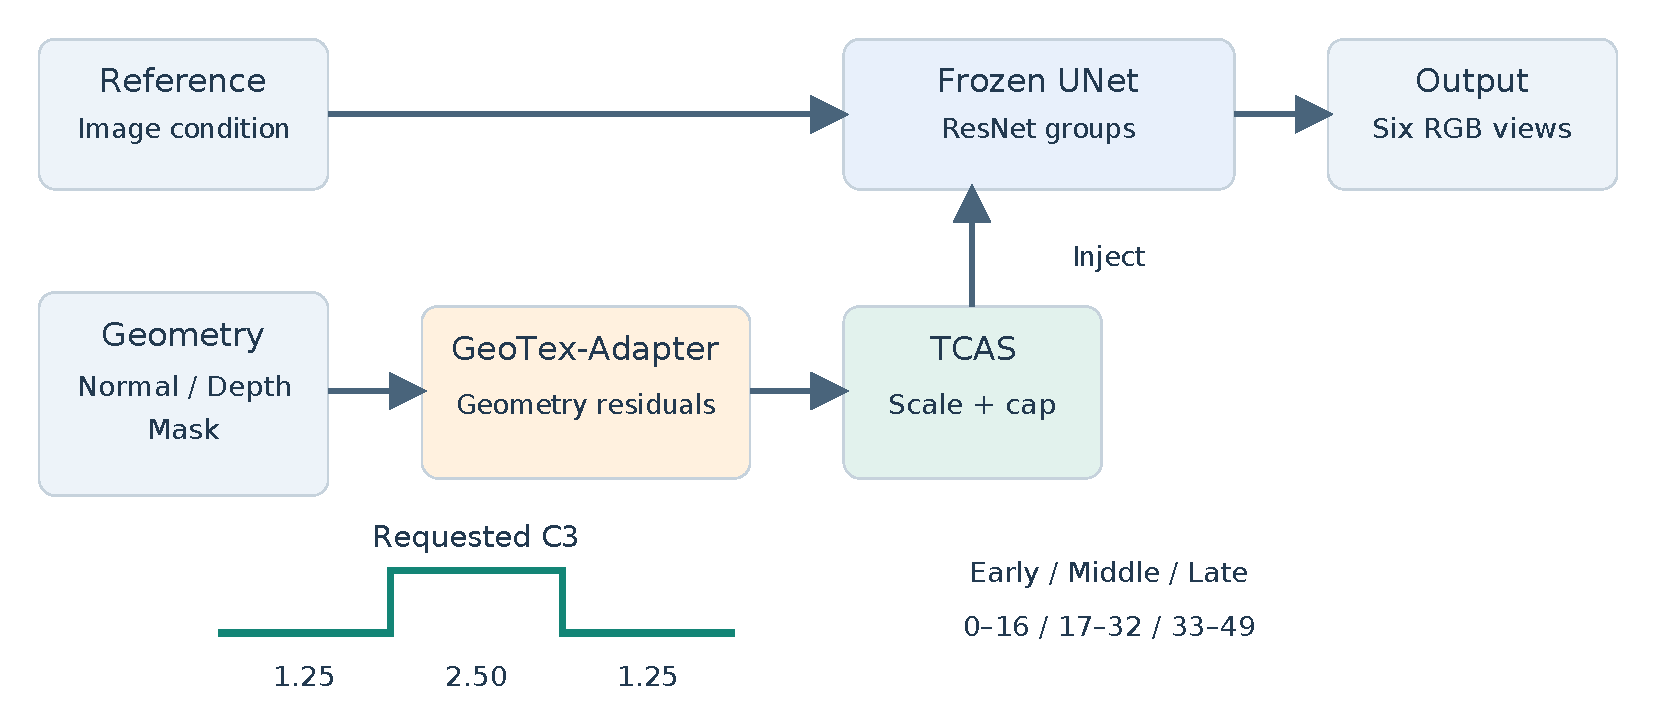
\includegraphics[width=\textwidth]{figures/fig1_tcas_control.pdf}
\DIFaddendFL \caption{\DIFdelbeginFL \DIFdelFL{Method overview. GeoTex-Adapter generates geometric residuals and injects them into UNet features. }\DIFdelendFL TCAS \DIFdelbeginFL \DIFdelFL{dynamically adjusts }\DIFdelendFL \DIFaddbeginFL \DIFaddFL{on }\DIFaddendFL the \DIFaddbeginFL \DIFaddFL{existing GeoTex }\DIFaddendFL residual \DIFdelbeginFL \DIFdelFL{strength according to denoising stages to balance geometric consistency }\DIFdelendFL \DIFaddbeginFL \DIFaddFL{path. Reference-image }\DIFaddendFL and \DIFdelbeginFL \DIFdelFL{texture fidelity}\DIFdelendFL \DIFaddbeginFL \DIFaddFL{five-channel geometry conditioning enter separate paths}\DIFaddendFL . \DIFdelbeginFL \DIFdelFL{FAC }\DIFdelendFL \DIFaddbeginFL \DIFaddFL{The requested C3 profile }\DIFaddendFL is \DIFdelbeginFL \DIFdelFL{an optional learned extension module}\DIFdelendFL \DIFaddbeginFL \DIFaddFL{$(1.25,2.50,1.25)$ over steps 0--16, 17--32 and 33--49; native group caps act before residual injection into the frozen UNet}\DIFaddendFL . \DIFdelbeginFL \DIFdelFL{The final multi-view outputs }\DIFdelendFL \DIFaddbeginFL \DIFaddFL{Fresh C shallow requests }\DIFaddendFL are \DIFdelbeginFL \DIFdelFL{projected }\DIFdelendFL \DIFaddbeginFL \DIFaddFL{capped at 0.8. This editable vector schematic abstracts multiple ResNet sites }\DIFaddendFL and \DIFdelbeginFL \DIFdelFL{baked into a textured 3D mesh}\DIFdelendFL \DIFaddbeginFL \DIFaddFL{is not an experimental result or end-to-end application demonstration}\DIFaddendFL .}
\label{fig:overview}
\end{figure*}

During multi-view diffusion, the 3D geometry is rendered into normal maps, depth maps, and foreground masks, denoted as:
\begin{equation}
\mathbf{G} = \{G_\text{normal}, G_\text{depth}, G_\text{mask}\}.
\end{equation}

The geometric adapter maps these conditions to a residual correction term and injects it into the intermediate hidden states of the UNet. For \DIFdelbegin \DIFdel{the $t$-th denoising step }\DIFdelend \DIFaddbegin \DIFadd{inference step $j$ with normalized execution progress $p_j$}\DIFaddend , the adapter injection can be written as:
\DIFdelbegin %DIFDELCMD < \begin{equation}
%DIFDELCMD < \mathbf{h}'_t = \mathbf{h}_t + s(p_t) \cdot A_\phi(\mathbf{h}_t, \mathbf{G}),
%DIFDELCMD < \label{eq:injection}
%DIFDELCMD < \end{equation}%%%
\DIFdelend \DIFaddbegin \begin{equation}
\mathbf{h}'_{j,\ell} = \mathbf{h}_{j,\ell} + s_{\mathrm{app}}(p_j,\ell)\, A^\ell_\phi(\mathbf{h}_{j,\ell}, \mathbf{G}),
\label{eq:injection}
\end{equation}\DIFaddend 
\DIFdelbegin \DIFdel{where $\mathbf{h}_t$ and $\mathbf{h}'_t$ denote the hidden states before and after injection,
$p_t$ denotes the sampling progress, and $s(p_t)$ is the adapter scaling strength at the current denoising stage. This formulation highlights a key difference from CFG-style guidance: changing $s(p_t)$ does not reweight two predicted scores, but changes the magnitude of a geometry-conditioned residual added to the feature stream. A larger $s$ usually enhances geometric condition adherence. However, if strong residuals are continuously applied in the late denoising stage, they may suppress the synthesis of color, material, }\DIFdelend \DIFaddbegin \DIFadd{Here $\ell$ indexes an injected layer group. The \emph{requested scale} $s_{\mathrm{req}}(p_j,\ell)$ is the value assigned by the profile; the \emph{applied scale} is the value used by the wrapper,
}\begin{equation}
s_{\mathrm{app}}(p_j,\ell)=\min\!\bigl(s_{\mathrm{req}}(p_j,\ell),c_\ell\bigr),
\end{equation}
\DIFadd{when the native cap $c_\ell$ is active, and otherwise equals the request. The resulting correction is $\mathbf{r}_{j,\ell}=s_{\mathrm{app}}(p_j,\ell)A^\ell_\phi(\mathbf{h}_{j,\ell},\mathbf{G})$; its \emph{post-scale residual magnitude} is $m_{j,\ell}=\|\mathbf{r}_{j,\ell}\|_2$. Thus neither a requested nor an applied scale label alone determines the correction magnitude.
}

\DIFadd{In the audited Fresh C wrapper, the three cap groups map the GeoTex residual wrappers on the UNet ResNet blocks as follows: deep comprises the UNet middle block and $\texttt{up\_0}$, middle is $\texttt{up\_1}$, and shallow is $\texttt{up\_2}$. These names identify the implementation's grouped injection points; they do not assert universal semantic roles for denoising stages. The corresponding Fresh C caps are 3.0, 3.5, }\DIFaddend and \DIFdelbegin \DIFdel{high-frequency details by the base diffusion model. This paper therefore studies how to schedule $s$ during denoising to balance shape consistency and texture detail preservation}\DIFdelend \DIFaddbegin \DIFadd{0.8. C3's shallow request of 1.25 is therefore applied as 0.8, while its deep and middle requests pass unchanged. GFL and GFH also clip at the shallow cap. These cap values describe the audited Fresh C wrapper; row-level cap semantics for the historical 24-object probe are not fully recoverable. TCAS scales a geometry residual added to feature activations; it does not reweight conditional and unconditional score predictions as classifier-free guidance does}\DIFaddend .

\DIFdelbegin %DIFDELCMD < \subsection{Shape-Texture Diagnostic Metrics}
%DIFDELCMD < %%%
\DIFdelend \DIFaddbegin \subsection{Image-Space Metrics and Texture-Variation Diagnostics}
\DIFaddend \label{subsec:metrics}

The \DIFdelbegin \DIFdel{influence of adapter scaling on generated results cannot be evaluated by a single structural metric. We divide evaluation metrics into three groups. The first group consists of shape and structure metrics, including FG-SSIM, Edge-SSIM, and }\DIFdelend \DIFaddbegin \DIFadd{endpoints describe different outcomes. \emph{Image-space agreement} refers to target-view PSNR, LPIPS, and SSIM measurements on the named image regions; it is not a measure of final 3D material quality. \emph{Reference-color agreement} refers to color differences such as CIEDE2000 computed against the corresponding reference. \emph{Texture variation} refers to statistics such as RGB standard deviation, Laplacian variance, gradient magnitude, and high-frequency energy; these may rise with detail or artifacts and are not fidelity measures. \emph{Subjective preference} refers only to the submitted forced-choice study. \emph{Baked 3D appearance} refers to rendered mesh outputs after texture projection or baking, while \emph{PBR/material fidelity} additionally concerns appearance under the material and illumination model. These endpoints are not interchangeable. FG-SSIM, Edge-SSIM, and }\DIFaddend Crop-SSIM \DIFdelbegin \DIFdel{, which measure consistency with ground-truth renderings in the foreground, edge regions, and local foreground crops based on the structural similarity index \cite{wang2004ssim}. The second group contains signal fidelity and perceptual similarity metrics, including PSNR and the learned perceptual image patch similarity (LPIPS) \cite{zhang2018lpips}, which reflect pixel-level errorand differences in deep feature space.
The third group consists of texture diagnostic metrics, including }\DIFdelend \DIFaddbegin \DIFadd{quantify structural similarity on the indicated image regions; PSNR measures pixel error; LPIPS compares learned image features \cite{wang2004ssim,zhang2018lpips}.
}

\DIFaddend Laplacian variance, RGB standard deviation, and gradient magnitude \DIFdelbegin \DIFdel{, which are used to detect weakened color variation, surface smoothing, and }\DIFdelend \DIFaddbegin \DIFadd{can describe local }\DIFaddend high-frequency \DIFdelbegin \DIFdel{detail loss. }%DIFDELCMD < 

%DIFDELCMD < %%%
\DIFdel{Taking Laplacian variance as an example, the foreground texture response is defined as
:
}%DIFDELCMD < \begin{equation}
%DIFDELCMD < M_\text{tex} = \text{Var}(\text{Lap}(I_\text{out} \odot G_\text{mask})),
%DIFDELCMD < \end{equation}%%%
\DIFdelend \DIFaddbegin \DIFadd{or color variation. For example, a foreground Laplacian statistic may be written as
}\begin{equation}
M_{\mathrm{var}}=\operatorname{Var}\!\left(\operatorname{Lap}(I_{\mathrm{out}}\odot G_{\mathrm{mask}})\right),
\end{equation}\DIFaddend 
where \DIFdelbegin \DIFdel{Lap denotes the Laplacian filter, $G_\text{mask}$ denotes }\DIFdelend \DIFaddbegin \DIFadd{$G_{\mathrm{mask}}$ is }\DIFaddend the foreground mask\DIFdelbegin \DIFdel{, and Var denotes spatial variance}\DIFdelend . A larger \DIFdelbegin \DIFdel{$M_\text{tex}$ usually corresponds to richer local high-frequency variation. If structural metrics improve while Laplacian variance, RGB standard deviation, or gradient magnitude decreases, the improvement may mainly come from contour smoothing or boundary convergence rather than true texture quality improvement}\DIFdelend \DIFaddbegin \DIFadd{value is not necessarily better: detail, noise, repeated patterns, or artifacts can all increase local variation. We therefore do not interpret these proxies as texture fidelity or use them alone to claim that a schedule better preserves reference appearance}\DIFaddend .

\DIFdelbegin %DIFDELCMD < \subsection{Timestep-Conditioned Adapter Scaling}
%DIFDELCMD < %%%
\DIFdelend \DIFaddbegin \subsection{TCAS Control Semantics and Comparison Design}
\DIFaddend \label{subsec:tcas}

\DIFdelbegin \DIFdel{The diffusion denoising process is stage-dependent: early steps mainly establish the global layout and coarse contours; middle steps refine geometric structure and cross-view alignment; late steps are more responsible for color, material, and local texture synthesis. Based on this observation, we propose Timestep-Conditioned Adapter Scaling (TCAS ), which }\DIFdelend \DIFaddbegin \DIFadd{TCAS }\DIFaddend replaces a globally fixed \DIFaddbegin \DIFadd{requested }\DIFaddend adapter scale with a \DIFdelbegin \DIFdel{stage-dependent scale function. TCAS is not intended as a generic smooth guidance schedule. Its low-high-low form encodes the adapter-specific hypothesis that geometry residuals should be strongest only after coarse structure becomes stable and before late texture synthesis dominates}\DIFdelend \DIFaddbegin \DIFadd{piecewise profile over normalized sampling progress. The early/middle/late partition is an operational description, not a universal claim about the function of every denoising stage. C3's low--high--low profile is the specific development choice evaluated in this revision; it is not presented as an independently derived optimum}\DIFaddend .

To avoid ambiguity caused by different raw timestep directions in different schedulers, \DIFdelbegin \DIFdel{we use sampling progress $p$ to represent the denoising process, where $p = 0$ denotes }\DIFdelend \DIFaddbegin \DIFadd{$p_j=j/(T-1)$ denotes execution progress for inference step $j\in\{0,\ldots,T-1\}$. Thus $p=0$ is the first update from }\DIFaddend the \DIFdelbegin \DIFdel{start from noise and $p = 1$ denotes the end of sampling close to the final image state. TCAS divides denoising into early, middle, and late stages:
}%DIFDELCMD < \begin{equation}
%DIFDELCMD < s(p) = \begin{cases} s_e, & 0 \leq p < 1/3 \\ s_m, & 1/3 \leq p < 2/3 \\ s_l, & 2/3 \leq p \leq 1 \end{cases}.
%DIFDELCMD < \label{eq:tcas}
%DIFDELCMD < \end{equation}%%%
\DIFdelend \DIFaddbegin \DIFadd{initial noisy latent and $p=1$ is the last denoising update before decoding. For $T=50$, TCAS divides execution into steps 0--16, 17--32, and 33--49 (17/16/17 steps):
}\begin{equation}
s_{\mathrm{req}}(p) = \begin{cases} s_e, & 0 \leq p < 1/3 \\ s_m, & 1/3 \leq p < 2/3 \\ s_l, & 2/3 \leq p \leq 1 \end{cases}.
\label{eq:tcas}
\end{equation}\DIFaddend 

\DIFaddbegin \DIFadd{We call this variation across the 50 inference steps the \emph{temporal allocation}. A \emph{layer allocation} varies the requested scale across the three wrapper groups at a fixed step. For a schedule with applied values $s_{\mathrm{app}}(j,\ell)$, its per-group applied-scale sum is $B_\ell=\sum_j s_{\mathrm{app}}(j,\ell)$; the unweighted sum $B_{\mathrm{nom}}=\sum_\ell B_\ell$ is a \emph{nominal applied-scale budget}. It does not weight scales by adapter activations. We log post-scale correction summaries, including wrapper-level $L_2$ norm and mean absolute entry. The three wrapper groups operate on feature maps with different spatial dimensions, and the traces do not retain channel counts; raw $L_2$ values are therefore not used for cross-layer dose comparisons. The per-entry mean absolute correction reported in Supplementary Section~S1 is a dimension-normalized descriptive summary, not an equal-dose intervention. Correction magnitudes also depend on the current hidden state and earlier denoising updates, so equal nominal budgets do not imply equal realized corrections.
}

\DIFaddend The selected C3 configuration used in this paper is:
\begin{equation}
(s_e, s_m, s_l) = (1.25, 2.50, 1.25).
\end{equation}

\DIFdelbegin \DIFdel{This design follows three principles. First, the early stage uses a conservative scale to avoid disrupting global structure formation with strong geometric residuals. Second, the middle stage uses a higher scale to strengthen geometric constraints from normals, depth maps, and foreground contours. Third, the late stage reduces the scale again to prevent geometric residuals from suppressing color variation, material detail, and high-frequency texture synthesis. This non-monotonic schedule is therefore different from simply decaying or increasing the adapter strength across all timesteps. TCAS introduces no new }\DIFdelend \DIFaddbegin \DIFadd{The low--high--low profile is a concrete inference-time intervention motivated by the submitted development analysis. Its stage interpretation is a task-specific hypothesis: the tested early, middle, and late allocations may produce different responses. Fresh C evaluates the recorded profile against matched controls but does not prove a universal function for any stage. TCAS adds no trained }\DIFaddend parameters and does not modify \DIFdelbegin \DIFdel{the base model }\DIFdelend \DIFaddbegin \DIFadd{base-model }\DIFaddend or adapter weights; it \DIFdelbegin \DIFdel{only replaces the scaling factor during inference, so its computational overhead is negligible}\DIFdelend \DIFaddbegin \DIFadd{replaces the requested scale during inference}\DIFaddend .

\DIFdelbegin %DIFDELCMD < \paragraph{Why mid-stage concentration is selected: the CAI model}
%DIFDELCMD < %%%
\DIFdel{The low--high--low form is not assumed but derived from a measurable Correction--Alignment--Interference (CAI) stage-utility model; we state the selection rule formally. Let $Q(s_e,s_m,s_l)$ denote a fidelity objective (PSNR here), let $L$ denote the fixed-low schedule, let $R$ denote the texture-deviation risk, given by the artifact-sensitive foreground texture diagnostics of Section~\ref{subsec:metrics} (Laplacian variance, RGB standard deviation, and gradient magnitude), and let $z_k\in\{0,1\}$ indicate whether the high scale is assigned to stage $k\in\{e,m,l\}$. Risk is compared by a non-worsening (Pareto) rule rather than a weighted scalarization: one assignment has lower risk than another only if it is no worse on every diagnostic and strictly better on at least one, so no artificial weights are introduced.
}%DIFDELCMD < 

%DIFDELCMD < \begin{proposition}[Guardrailed $\epsilon$-optimal selection]
%DIFDELCMD < \label{prop:cai}
%DIFDELCMD < %%%
\DIFdel{Suppose (i) the stage-utility model $Q(s_e,s_m,s_l)=Q(L)+\sum_{k}U_k z_k$, where $U_k=Q(\text{high scale only in }k)-Q(L)$ is the measured finite-difference utility of stage $k$, and (ii) per-stage guardrails under which stage $k$ is admissible for }\DIFdelend \DIFaddbegin \paragraph{What C3 changes and what its comparisons identify}
\DIFadd{C3 requests $(1.25,2.50,1.25)$ for each of the 50 steps across the three layer groups before native caps. In Fresh C, }\DIFaddend the \DIFdelbegin \DIFdel{high scale only if its intervention does not reduce FG-SSIM by more than $\tau$ nor raise the texture-deviation risk beyond a factor $\rho$ relative to $L$. Selection proceeds in two stages.
First, maximize fidelity over the admissible schedules $\mathcal{F}$: the fidelity-optimal assignment is $z_k^{\mathrm{fid}}=\mathbf{1}[\,U_k>0 \text{ and } k \text{ admissible}\,]$, with value $Q_{\max}=\max_{z\in\mathcal{F}}Q(z)$. Second, restrict attention to the $\epsilon$-equivalent set $\mathcal{F}_\epsilon=\{\,z\in\mathcal{F}: Q(z)\ge Q_{\max}-\epsilon\,\}$ for a small fidelity-equivalence margin $\epsilon>0$, and select $z^{\star}=\arg\min_{z\in\mathcal{F}_\epsilon}R(z)$. Then: an inadmissible stage is fixed at the conservative scale; any admissible stage whose estimated utility alone exceeds $\epsilon$ must retain the high scale; and a stage whose estimated utility satisfies $0<U_k<\epsilon$, with a structurally insignificant change, is fidelity-equivalent under either assignment, so the risk-dominant conservative scale is selected. Measured confidence intervals serve as auxiliary uncertainty information and do not enter the membership condition of $\mathcal{F}_\epsilon$. }%DIFDELCMD < \end{proposition}
%DIFDELCMD < 

%DIFDELCMD < \begin{quote}\small
%DIFDELCMD < %%%
\DIFdel{\textit{Proof.} Under (i), for any $z\in\mathcal{F}$, $Q(z)=Q_{\max}-\sum_{k:\,z_k^{\mathrm{fid}}=1}U_k\,(1-z_k)$, so $z\in\mathcal{F}_\epsilon$ exactly when the total positive utility dropped by reassigning high-scale stages to the conservative scale does not exceed $\epsilon$. Condition (ii) fixes $z_k=0$ for inadmissible stages and leaves the admissible stages independent, so each stage can be examined separately. A stage with $U_k>\epsilon$ cannot be dropped from the fidelity optimum without leaving $\mathcal{F}_\epsilon$, hence $z_k^{\star}=1$. A stage with estimated utility $0<U_k<\epsilon$ contributes at most $\epsilon$ when dropped, so both assignments lie in $\mathcal{F}_\epsilon$; within $\mathcal{F}_\epsilon$ the second selection stage minimizes texture-deviation risk, and for such a stage the structural change is insignificant while the conservative scale strictly reduces the risk, so $z_k^{\star}=0$.
}%DIFDELCMD < \hfill%%%
\DIFdel{$\square$
}%DIFDELCMD < \end{quote}
%DIFDELCMD < %%%
\DIFdelend \DIFaddbegin \DIFadd{applied deep and middle profiles retain those values; the shallow profile is clipped to 0.8 throughout. GFL requests 1.25 at every step and group, so its deep and middle values are 1.25 throughout and its shallow value is also clipped to 0.8. Their per-group applied-scale sums are therefore 82.5 versus 62.5 in deep and middle, and 40 for both in shallow. The C3--GFL contrast changes the middle-third deep/middle scale magnitude as well as its temporal allocation; it is not a timing-only comparison.
}\DIFaddend 

\DIFdelbegin %DIFDELCMD < \begin{remark}
%DIFDELCMD < %%%
\DIFdel{The utilities are measured finite differences on a 24-object stage ablation of the strong-residual, per-layer-capped adapter instance (regime~(b) of Section~\textit{[removed reference: }\texttt{subsec:adapterdep}\textit{]}), where per-stage effects are most visible: $U_e=-0.788$~dB (95\% CI $[-1.420,-0.156]$) with a guardrail violation (FG-SSIM $-0.105$, CI $[-0.141,-0.069]$; foreground Laplacian variance $3.85\times$ fixed-low), $U_m=+0.574$~dB $[0.391,0.756]$, and $U_l=+0.077$~dB $[0.006,0.149]$ with a structurally insignificant FG-SSIM change ($+0.001$, CI $[-0.002,0.003]$). Proposition~\textit{[removed reference: }\texttt{prop:cai}\textit{]} selects exactly the conservative--high--conservative assignment C3: the early stage is inadmissible, the middle stage must retain the high scale because its utility alone ($+0.574$~dB) exceeds any meaningful equivalence margin such as $\epsilon=0.1$~dB, and the late stage has estimated utility $U_l=0.077<\epsilon=0.1$~dB while its FG-SSIM change is statistically insignificant, so removing the late high-scale intervention remains within the $\epsilon$-equivalent fidelity set and reduces texture risk; the risk-dominant conservative scale is therefore selected. The same conservative--high--conservative assignment is independently selected by the main adapter's 17-variant probe (Table~\textit{[removed reference: }\texttt{tab:probe}\textit{]}); the utilities above explain, rather than determine, that selection, and Remark~2 delimits the conditional scope of this explanation.
}%DIFDELCMD < \end{remark}
%DIFDELCMD < %%%
\DIFdelend \DIFaddbegin \DIFadd{To identify a temporal-placement contrast, controls must hold the per-layer applied values and nominal per-group sums fixed while moving the same values between time windows. To identify a scale-strength contrast, controls must hold the layer and temporal allocations fixed while changing amplitude. Both contrasts also require reporting post-scale correction summaries: matching requested values or applied-scale sums does not match the evolving residual corrections. Raw $L_2$ values are dimension-sensitive across wrapper groups and cannot establish cross-layer dose matching. The current 300-object allocation comparison exactly matches the applied sums in each layer group. This controls the scalar budget for the total allocation effect, although it does not identify a residual-dose-independent mechanism. Post-hoc adjustment for state-dependent corrections cannot by itself recover that mechanism. The older strict-276 analysis is reported separately.
}\DIFaddend 

\DIFdelbegin %DIFDELCMD < \begin{remark}
%DIFDELCMD < %%%
\DIFdel{Additivity is an approximation: stage effects interact, and the complete }\DIFdelend \DIFaddbegin \paragraph{Development origin and scope of C3}
\DIFadd{The submitted 01549 paper records }\DIFaddend C3 \DIFdelbegin \DIFdel{schedule is therefore validated directly (Secs.~\ref{subsec:c3}--\textit{[removed reference: }\texttt{subsec:adapterdep}\textit{]}). Changing the adapter, its residual magnitude, or the scale semantics changes the measured $U_k$ and requires re-estimation. Proposition~\textit{[removed reference: }\texttt{prop:cai}\textit{]} thus provides a conditional decision rule within the measured adapter regime---explaining why the mid-stage assignment follows from data rather than from a hand-tuned rule---and not a universal guarantee.
}%DIFDELCMD < \end{remark}
%DIFDELCMD < 

%DIFDELCMD < \subsection{GeoTex-Adapter and FAC Adaptive Extension}
%DIFDELCMD < \label{subsec:fac}
%DIFDELCMD < 

%DIFDELCMD < %%%
\DIFdel{GeoTex-Adapter, TCAS, and FAC correspond to three complementary dimensions of adapter control. GeoTex-Adapter determines what geometric residual correction should be injected. TCAS determines when the residual should be strengthened or weakened along the denoising-time dimension. FAC further modulates the residual in a fine-grained manner along spatial positions and frequency components}\DIFdelend \DIFaddbegin \DIFadd{$=(1.25,2.50,1.25)$ as the selected profile from a 24-object development probe containing 17 uniform, layer-wise, and time-conditioned variants. We retain that development record because it explains the origin of the profile studied here. The complete row-level outputs and selection-time provenance are not available in the current evidence authority, so the historical ranking and labels cannot be independently checked. We therefore make no formal optimality or uniqueness claim based on this probe. Fresh C evaluates the recorded profile without further schedule search}\DIFaddend .

\DIFaddbegin \subsection{Geometry Adapter and Inference Interface}
\label{subsec:adapterimpl}

\DIFaddend GeoTex-Adapter is \DIFdelbegin \DIFdel{used as a fixed geometric residual backbone}\DIFdelend \DIFaddbegin \DIFadd{treated as the fixed geometry-residual backbone, not as a new contribution of this paper}\DIFaddend . It receives a \DIFdelbegin \DIFdel{5-channel geometric input consisting of a 3-channel }\DIFdelend \DIFaddbegin \DIFadd{five-channel input comprising a three-channel }\DIFaddend normal map, a \DIFdelbegin \DIFdel{1-channel }\DIFdelend \DIFaddbegin \DIFadd{one-channel }\DIFaddend depth map, and a \DIFdelbegin \DIFdel{1-channel }\DIFdelend \DIFaddbegin \DIFadd{one-channel }\DIFaddend foreground mask. A multi-scale \DIFdelbegin \DIFdel{geometric encoder produces a feature pyramid, and residual corrections }\DIFdelend \DIFaddbegin \DIFadd{encoder produces residual features that }\DIFaddend are injected into \DIFdelbegin \DIFdel{multiple resolution levels of the }\DIFdelend \DIFaddbegin \DIFadd{the frozen }\DIFaddend UNet. TCAS acts on the \DIFdelbegin \DIFdel{global temporal scale of these residuals to control the influence of geometric conditions at different denoising stages without changing the adapterarchitecture}\DIFdelend \DIFaddbegin \DIFadd{requested multiplier along denoising progress; it does not retrain the adapter, the UNet, or the VAE and introduces no learned parameters}\DIFaddend .

\DIFdelbegin \DIFdel{To further examine whether stage-wise adapter control can be extended to learned adaptive correction, we also conduct experiments with }\DIFdelend \DIFaddbegin \DIFadd{Previously reported }\DIFaddend Full Adaptive Correction (FAC) \DIFdelbegin \DIFdel{. FAC contains three lightweight modules: LTAG learns timestep-dependent gating, GSG generates spatial gates from geometric features, and FSC performs frequency-selective correction on adapter residuals.
Unlike fixed TCAS, FAC finely modulates adapter residuals in the temporal, spatial, and frequency domains. In the extension experiments, FAC uses TCAS as the base temporal schedule and further adds GSG and FSC for spatial and frequency correction.
}\DIFdelend \DIFaddbegin \DIFadd{training is retained as an auxiliary negative result in Section~\ref{subsec:facreported}. It is distinct from the frozen inference interventions evaluated here.
}\DIFaddend 

\DIFdelbegin \DIFdel{It should be emphasized that FAC requires learning a small number of additional parameters. Therefore, TCAS,which requires no training , remains the main method in this paper. FAC is used only as a learned adaptive extension; Section~\textit{[removed reference: }\texttt{subsec:facexp}\textit{]} reports a controlled re-examination that delimits when learned modulation can be expected to help}\DIFdelend \DIFaddbegin \DIFadd{The recorded analysis and display code uses fixed object-level inputs and the original comparison families. Actual experimental images are preserved without appearance retouching. Software identities and the AI-assistance disclosure are supplied with the reproduction materials. Final displays are checked against source hashes, shared cameras/crops and object-level metrics; visual assessment illustrates appearance limitations and is not an additional quality endpoint}\DIFaddend .

\section{Experiments}
\label{sec:experiments}

\DIFdelbegin %DIFDELCMD < \subsection{Experimental Setup}
%DIFDELCMD < %%%
\DIFdelend \DIFaddbegin \subsection{Study Cohorts, Sampling and Statistical Units}
\DIFaddend \label{subsec:setup}

\DIFdelbegin %DIFDELCMD < \subsubsection{Experimental protocol and comparisons}
%DIFDELCMD < %%%
\DIFdelend \DIFaddbegin \DIFadd{Table~\ref{tab:study-design} separates the studies and their evidence classes. Fresh C contains 300 UIDs disjoint from the historical schedule-selection/evaluation pool, the recorded 1,118-object training list and the earlier clean-v2 evaluation list. Its primary four-condition comparison uses one frozen controlled-retraining checkpoint, shared inputs and per-object seeds. It does not reproduce the historical adapter's reported $+0.96$ dB estimate. The original checkpoint's exact identity remains unavailable.
}\DIFaddend 

\DIFdelbegin \DIFdel{Experiments are conducted using an MVPainter-style geometry-controlled multi-view diffusion pipeline. Each objectcontains a single reference image and corresponding 3D geometry. During preprocessing, the 3D geometry is rendered into target-view normal maps, depth maps, foreground masks, and ground-truth RGB images. The model generates six target views at a time, and all comparisons with ground-truth renderings are performed under unified views, resolution, and foreground masks}\DIFdelend \DIFaddbegin \begin{table*}[t]
\centering\scriptsize\setlength{\tabcolsep}{3pt}
\caption{Studies, implemented protocols and evidence scope. Rows are studies rather than disjoint populations: the bake pilots and some interface tests reuse image-study inputs. Object is the statistical unit; views and seeds are nested within object.}
\label{tab:study-design}
\begin{tabular}{p{0.16\textwidth}p{0.23\textwidth}p{0.20\textwidth}p{0.32\textwidth}}
\toprule Study / objects & Interface and sampling & Endpoint & Selection and scope \\
\midrule
Fresh C / 300 & Capped GeoTex residual; 256 pixels; 50 Euler steps; conditional-only prediction; cached image features & Six target-view foreground endpoints & UID-disjoint held-out cohort; original primary C3--GFL frozen; linear and equal-budget comparisons are same-cohort addenda \\
GeoTex bake / 10 & Same controlled generator; six 256-pixel bake cameras; native UVs & Eleven unseen unlit views & Input/compatibility-selected subset; primary Late--Mean specified before new bake outcomes; two later native controls exploratory \\
MV-Adapter / 50 & Native condition-guider features; 512 pixels; 50 steps; CFG 3 & Six native-camera target views & Fresh C inputs not previously viewed through this interface; input-only selection; thirteen legal white targets retained \\
GSO / 100 & Native MV-Adapter; 512 pixels; 50 steps; CFG 3; three seeds & All-six PSNR primary; five nonreference LPIPS secondary & Source-ordered convenience cohort; four inherited profiles frozen after earlier baseline exposure; external sensitivity \\
GSO bake / 20 & Same fixed GSO inputs; native UVs; three seeds & Eleven unseen unlit views & Revised GT-only calibration after fifteen original outcomes; full twenty retained; no GT-error subtraction \\
Reference-protocol / 50 & New frozen GeoTex checkpoint; native reference conditions; 512 pixels; 50 steps; CFG 2 & Five nonreference views & Supporting protocol/checkpoint sensitivity on previously studied inputs; not another independent backbone \\
MVDiffusion / 75 & Partial correspondence-block control; depth concatenation unscaled & Recorded six-view endpoints & Retrospective third-interface panel; narrow native-mirror identity check; not exact GeoTex operator transfer \\
\bottomrule
\end{tabular}
\end{table*}

\DIFadd{Within each comparison, object inputs, targets, initialization and endpoint code are shared. Fresh C uses seed $42+\texttt{object\_idx}$, held constant across conditions for that object. Its capped residual groups have deep/middle/shallow limits of 3.0/3.5/0.8}\DIFaddend . \DIFaddbegin \DIFadd{MV-Adapter uses a different feature injection operator and numerical scale range; its native target cameras and actual default-path identity are checked separately. Scale labels are not common physical doses across interfaces.
}\DIFaddend 

\DIFdelbegin \DIFdel{Except for the FAC extension experiment, all scaling experiments keep the object list, reference image , target views, random seed, base UNet, VAE, adapter weights, and number of denoising steps fixed; only the adapter scale or schedule is changed. The number of sampling steps is 50. }\DIFdelend \DIFaddbegin \DIFadd{Fresh C's controlled sampler differs from the complete base pipeline, which uses online image features, classifier-free guidance and 512-pixel views. Constant 1.0 under the GeoTex caps also differs from the unset-scale residual branch. We therefore name these controls by their executed configuration. The source records and sampling/default-path diagnostics are in Supplementary Sections~S1 and S6.
}

\DIFadd{FG-PSNR, LPIPS, SSIM and Edge-SSIM measure agreement on the named image regions. Baked evaluation renders actual exported meshes; unlit base color does not establish PBR or material fidelity. Fresh C image endpoints are evaluated once on each frozen $3\times2$ six-view composite. Native-interface and baked endpoints average their recorded per-view scores within object, with GSO sampling seeds also averaged within object. Paired intervals resample objects and are pointwise 95\% intervals. Preserved primary, secondary and exploratory families use their stated Holm adjustments; the distinct families do not imply one overall experiment-wide error guarantee. Non-detection is not equivalence or non-inferiority. Complete comparison rules are supplied in Supplementary Sections~S2--S5.
}

\subsection{Development origin and historical scope}
\label{subsec:c3}
\DIFadd{The historical study selected }\DIFaddend C3 \DIFdelbegin \DIFdel{is selected using only }\DIFdelend \DIFaddbegin \DIFadd{from 17 profiles on }\DIFaddend a 24-object probe \DIFdelbegin \DIFdel{set; the same schedule is then frozen and applied to the 300-object evaluation pool, where no parameter search is performed. This probe-to-pool protocol isolates the effect of adapter scaling from changes in model architecture, training data, sampling budget, or evaluation-set tuning. }%DIFDELCMD < 

%DIFDELCMD < %%%
\DIFdel{Accordingly, the comparisons in this paper are comparisons among inference-time adapter scaling strategies under the same base pipeline, rather than a system-level benchmark among different texture generation architectures.
Uniform adapter scales serve as the primary deployment baselines because they correspond to the most direct way of choosing a single fixed adapter strength at inference time. The probe variants further test whether the trade-off can be resolved by simple alternatives such as globally high scales, layer-wise redistribution, or moving high adapter strength to early, late, or multiple denoising stages. TCAS changes only how this strength is scheduled across denoising stages.
}\DIFdelend \DIFaddbegin \DIFadd{and reported a separate fixed-scale sweep. Those records explain the intervention's origin, but their complete row-level provenance cannot be reconstructed. They remain historical diagnostics in Supplementary Section~S7. The current matched evaluation carries C3 forward without another selection search. Historical pooled gains, preference and FAC results remain separate from the new evidence.
}\DIFaddend 

\DIFdelbegin %DIFDELCMD < \subsubsection{Evaluation sets and metrics}
%DIFDELCMD < %%%
\DIFdelend \DIFaddbegin \subsection{Competitive Controls and Matched Temporal Allocation}
\label{subsec:largescale}
\DIFaddend 

\DIFdelbegin \DIFdel{We use four evaluation sets: (1) a 50-object scale-sweep set for analyzing the overall trend of structural metrics under 13 uniform scales; (2) a 26-object texture audit set for comparing texture degradation under $s = 1.25$ and $s = 2.50$; (3) a 24-object probe set for evaluating 17 uniform, layer-wise, and timestep-conditioned scheduling variants and selecting }\DIFdelend \DIFaddbegin \DIFadd{The internally specified Fresh C primary is }\DIFaddend C3 \DIFdelbegin \DIFdel{; and (4)a 300-object evaluation pool, comprising the 24-object probe and a 276-object held-out subset (detailed below), for testing the selected }\DIFdelend \DIFaddbegin \DIFadd{minus Fixed Low (GFL) FG-PSNR. The paired gain is $+0.52$ dB (95\% interval $[+0.40,+0.64]$), with 206/300 objects favorable. All conditions use the same frozen retrained checkpoint and object inputs. This gain combines increased strength and temporal allocation: }\DIFaddend C3\DIFdelbegin \DIFdel{schedule, uniform baselines, and the FAC extension without any further schedule search. }\DIFdelend \DIFaddbegin \DIFadd{'s deep/middle applied sums are 82.5 each, versus 62.5 for GFL, while both have shallow sum 40.
}\DIFaddend 

\DIFdelbegin \DIFdel{Evaluation metrics are divided into three categories: shape and structure metrics (FG-SSIM}\DIFdelend \DIFaddbegin \begin{table*}[t]
\centering\scriptsize\setlength{\tabcolsep}{4pt}
\caption{Fresh C competitive-control means on the same 300 objects. Early/Middle/Late-high and Fixed Mean share exactly the same per-group applied sums. The equal-budget study is a post-inspection addendum, not a second holdout. Each budget entry for deep/middle applies separately to both groups. $^\dagger$Generic Linear is a competitive same-cohort addendum, not part of the matched-budget family; its different group budgets are shown explicitly.}
\label{tab:freshc-absolute}\label{tab:matched-budget300}
\begin{tabular}{lrrrrrr}
\toprule Control & Deep/middle sum & Shallow sum & FG-PSNR$\uparrow$ & FG-LPIPS$\downarrow$ & FG-SSIM$\uparrow$ & Edge-SSIM$\uparrow$ \\
\midrule
Fixed Low & 62.5 & 40 & 11.31 & 0.2051 & 0.3500 & 0.4728 \\
Fixed High & 125.0 & 40 & 12.58 & 0.1891 & 0.4201 & 0.4961 \\
Fixed Mean & 82.5 & 40 & 11.96 & 0.1978 & 0.3864 & 0.4843 \\
Early-high & 82.5 & 40 & 11.33 & 0.2045 & 0.3696 & 0.4765 \\
C3 / Middle-high & 82.5 & 40 & 11.83 & 0.1998 & 0.3746 & 0.4773 \\
Late-high & 82.5 & 40 & 12.39 & 0.1951 & 0.3788 & 0.4914 \\
Generic Linear$^\dagger$ & 93.75 & 31.25 & 12.42 & 0.1862 & 0.4026 & 0.4880 \\

\bottomrule
\end{tabular}
\end{table*}

\DIFadd{Competitive controls change the recommendation. Fixed High has better means than C3 on all four endpoints: C3 minus Fixed High is $-0.748$ dB FG-PSNR (pointwise interval $[-0.885,-0.609]$)}\DIFaddend , \DIFdelbegin \DIFdel{Edge-SSIM,and Crop-SSIM),signal and perceptual metrics (PSNR and LPIPS), and texture diagnostic metrics (Laplacian variance, RGB standard deviation, and gradient magnitude). All metrics are first computed over six target views and then averaged over views and objects. For texture-related conclusions, we report means, }\DIFdelend \DIFaddbegin \DIFadd{with FG-SSIM difference $-0.04553$ ($[-0.04937,-0.04167]$). Generic Linear ramps deep/middle requests from 1.25 to 2.50 and shallow requests from 0.50 to 0.75 over the fifty steps. Its applied sums are (93.75,93.75,31.25), so it changes layer allocation and total budget as well as timing. It also has better means on all four; C3 minus Generic Linear is $-0.593$ dB ($[-0.837,-0.351]$). Its positive median of $+0.074$ dB and 155/300 favorable objects show why mean and }\DIFaddend object-level \DIFdelbegin \DIFdel{win rates, and significance tests to avoid judging generation quality based on a single structural score}\DIFdelend \DIFaddbegin \DIFadd{distributions must both be considered. Complete original paired endpoints and their comparison families are in Supplementary Section~S2}\DIFaddend .

\DIFdelbegin \DIFdel{The FAC extension uses the same object list and evaluation protocol as the 300-object evaluation pool, and its lightweight modules are trained only on the 1, 706-object training pool for the strong-residual adapter instance, which is disjoint from all evaluation objects. TCAS is used as the main baseline, while LTAG, LTAG+GSG, and Full FAC are evaluated as ablation variants under the same paired protocol. The base model and original adapter remain frozen,}\DIFdelend \DIFaddbegin \paragraph{Equal applied budgets.}
\label{subsec:matched-budget300}
\DIFadd{Early-, middle-, and late-high move the same sixteen high steps to updates 0--15, 17--32, }\DIFaddend and \DIFdelbegin \DIFdel{only lightweight adaptive correction parameters are learned}\DIFdelend \DIFaddbegin \DIFadd{34--49. Deep/middle low and high are 1.25 and 2.50; shallow stays at its 0.8 cap. Fixed Mean uses 1.65 before the cap. Each allocation therefore has per-group sums $(82.5,82.5,40)$. The completed six-condition matrix contains 1,800 paired rows with common-input and seed checks}\DIFaddend .

\DIFdelbegin %DIFDELCMD < \subsubsection{Implementation and dataset details}
%DIFDELCMD < %%%
\DIFdelend \DIFaddbegin \DIFadd{C3 minus Fixed Mean is $-0.133$ dB (pointwise interval $[-0.170,-0.096]$); C3 minus Late-high is $-0.564$ dB ($[-0.634,-0.494]$). C3 also trails both on LPIPS, FG-SSIM and Edge-SSIM. It improves over Early-high by approximately 0.50 dB. Within these six conditions Fixed High wins FG-PSNR on 172 objects, Late-high on 64, and C3 on none; this is an endpoint-specific count, not a universal quality ranking.
}\DIFaddend 

\DIFdelbegin \DIFdel{All objects are drawn from the Objaverse 3D asset collection: ground-truth multi-view images are rendered offline with Blender (Cycles engine, 17 views at $512\times512$, white background), and six target views (front, front-right, right, back, left, front-left)are used throughout the paper. The main adapter's training pool contains 1}%DIFDELCMD < {%%%
\DIFdel{,}%DIFDELCMD < }%%%
\DIFdel{118 rendered objects, while the strong-residual v2 instance used in Section~\textit{[removed reference: }\texttt{subsec:adapterdep}\textit{]} and the FAC experiments is trained on a separate 1}%DIFDELCMD < {%%%
\DIFdel{, }%DIFDELCMD < }%%%
\DIFdel{706-object pool from the same source. Both training pools are disjoint from the evaluation pool; we verified that each training}\DIFdelend \DIFaddbegin \DIFadd{A descriptive four-endpoint comparison complements these winner counts. On 270}\DIFaddend /\DIFdelbegin \DIFdel{evaluation identifier intersection is zero. Within the 300-object evaluation pool, the 24-object probe set corresponds to the first 24 identifiers ($\mathrm{obj}_{0000}$--$\mathrm{obj}_{0023}$) and the remaining 276 identifiers ($\mathrm{obj}_{0024}$--$\mathrm{obj}_{0299}$) form a holdout that is strictly disjoint from the probe; Section~\textit{[removed reference: }\texttt{subsec:adapterdep}\textit{]} reports transfer statistics on this disjoint holdout for the strong-residual, per-layer-capped adapter instance, in addition to the full-pool tables.
The 50-object scale-sweep set comprises the first 50 objectsof the pool ($\mathrm{obj}_{0000}$--$\mathrm{obj}_{0049}$), and the 26-object audit set is a purposive subset of these 50 objects, selected to span the observed range of per-object $\Delta$FG-SSIM behavior for manual inspection; all evaluation sets are subsets of the 300-object pool, and no training object appears in any of them}\DIFdelend \DIFaddbegin \DIFadd{300 objects, at least one of the other five controls weakly dominates C3 on all four recorded composite endpoints and improves at least one. Fixed High alone does so on 173 objects, but C3 dominates it on 16; their remaining 111 objects have competing endpoints. This post-inspection, point-estimate analysis is not statistical separation on each object or a ranking of unmeasured material quality. Full counts are in Supplementary Section~S2}\DIFaddend .

The \DIFdelbegin \DIFdel{base pipeline is an MVPainter-style geometry-controlled multi-view diffusion model built on a joint six-view latent UNet, loaded from the local \texttt{MVPainter\_Pipeline} snapshot under \texttt{checkpoints/hf\_repo} with diffusers 0.20.0, and used frozen together with its VAE. The pipeline is reference-image-conditioned; no text prompts are used. The GeoTex-Adapter takes a five-channel geometric input (3-channel normal map, 1-channel depth map, 1-channel foreground mask), produces a multi-scale residual pyramid, and injects corrections into multiple UNet resolution levels; for the adapter studied in the main tables, the requested scale is applied multiplicatively at every injected layer.
Inference uses the Euler discrete scheduler with 50 denoising steps and a fixed random seed (42) shared by all schedules within an experiment, so all variants share the same initial latents; the model generates six views per object.
}%DIFDELCMD < 

%DIFDELCMD < %%%
\DIFdel{FG-SSIM, Edge-SSIM (edge masks derived from depth}\DIFdelend \DIFaddbegin \DIFadd{equal-budget comparison identifies an allocation total effect. Evolving residual amplitudes remain trajectory-dependent, preventing a residual-dose-independent mechanism interpretation. Late-high is not universally preferred: Fixed Mean has higher FG-SSIM, and Generic Linear is a strong unmatched-budget practical control. The historical LLH layer}\DIFaddend /\DIFdelbegin \DIFdel{normal discontinuities), PSNR, and LPIPS (AlexNet backbone) are computed on foreground-masked regions after background normalization; the texture diagnostics (foreground Laplacian variance, RGB standard deviation, gradient magnitude) are computed on foreground pixels and compared against the same ground-truth renderings under identical views and masks. The main tables use GeoTex-Adapter \texttt{geotex\_refattn\_v1/geotex\_step\_0002000.pt} trained on the 1}%DIFDELCMD < {%%%
\DIFdel{,}%DIFDELCMD < }%%%
\DIFdel{118-object pool; the strong-residual analyses use \texttt{mvpoutput/geotex\_v2/checkpoints/geotex\_v2\_ema\_final.pt} (MD5 \texttt{a74cc1d16cb473a95022bdcbc58e1b22})trained on the 1}%DIFDELCMD < {%%%
\DIFdel{,}%DIFDELCMD < }%%%
\DIFdel{706-object pool. The checkpoint files and evaluation code will be made available upon reasonable request, and a consolidated reproducibility table (data subsets, checkpoint identifiers, scheduler,seed, }\DIFdelend \DIFaddbegin \DIFadd{time addendum and complete object distributions remain in Supplementary Section~S2.
}

\begin{figure*}[!t]
\centering
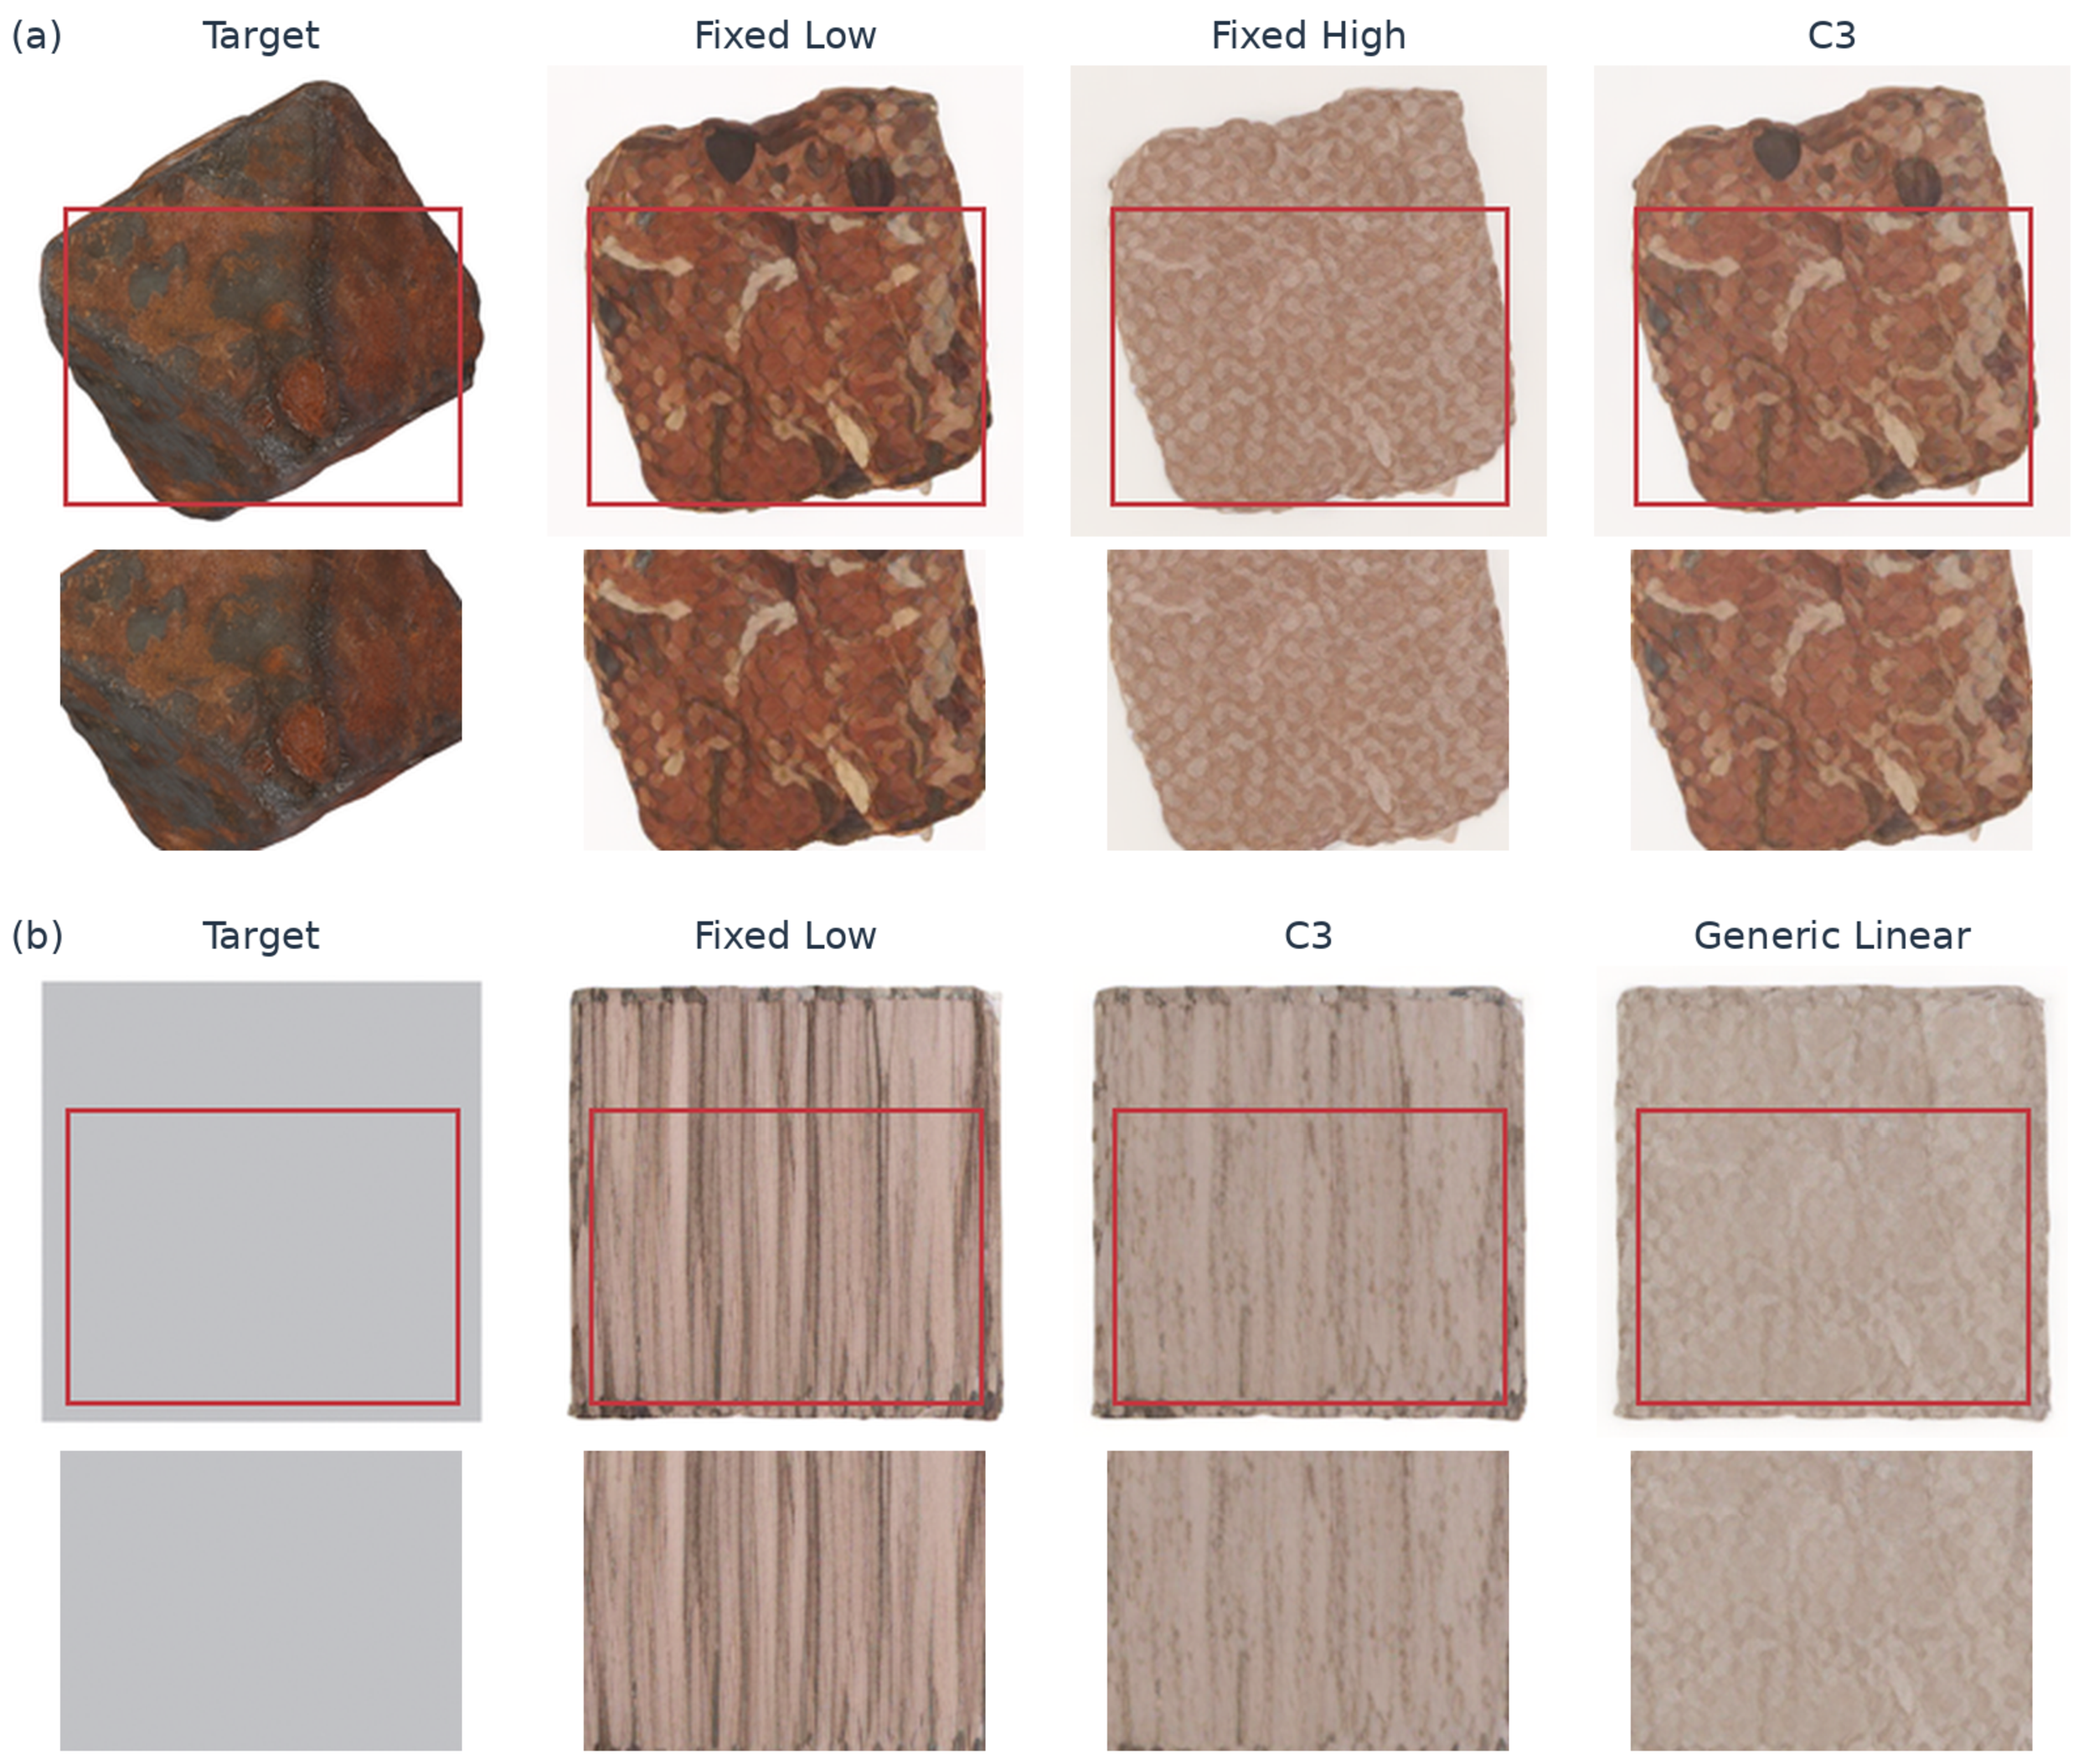
\includegraphics[width=\textwidth]{figures/fig5_freshc_context_roi.pdf}
\caption{\DIFaddFL{Fresh C view 0: (a) Octa\`edre, a fixed-scale endpoint trade-off; (b) Cube 01, a Generic Linear counterexample. Each column shows the complete object in a common frame and the same pixel ROI enlarged below. Object-level C3 minus Generic Linear in (b) is $-3.491$~dB FG-PSNR and $+0.08172$ FG-LPIPS, favoring Linear on both. Added patterns visibly differ from the low-variation target. These retained outcome-selected examples illustrate behavior, not prevalence or material fidelity. Composite object metrics use all six views, not only the displayed crop. Source hashes, camera/seed identities and display frames are in the final visual manifest; credits are in Supplementary Section~S9.}}
\label{fig:c3compare}
\end{figure*}


\subsection{Appearance and Color Failure Analysis}
\label{subsec:appearance-color}

\DIFadd{The selected color diagnosis contains 26 failure-enriched objects: six earlier figure cases and 20 Fresh C panels. It is not a random sample, a new holdout, or a population estimate. No Adapter, GFL, and LLH were compared on the same inputs, checkpoint, }\DIFaddend and \DIFdelbegin \DIFdel{metric implementations) is provided in the supplementary material}\DIFdelend \DIFaddbegin \DIFadd{runner with six target views per object (78 object-condition records)}\DIFaddend . \DIFdelbegin %DIFDELCMD < 

%DIFDELCMD < \paragraph{Statistical reporting}
%DIFDELCMD < %%%
\DIFdel{Object-level paired comparisons report two-sided paired tests and 95\% confidence intervals constructed by percentile bootstrap over objectswith 10}%DIFDELCMD < {%%%
\DIFdel{, }%DIFDELCMD < }%%%
\DIFdelend \DIFaddbegin \DIFadd{The following paired object-bootstrap intervals are descriptive (20,}\DIFaddend 000 \DIFdelbegin \DIFdel{resamples.Where a mean is accompanied by $\pm$, the quantity is the standard deviation across objects. Preference-study intervals add a participant-level bootstrap level (Section~\ref{subsec:largescale}). }%DIFDELCMD < 

%DIFDELCMD < \subsection{Shape-Texture Trade-off of Adapter Scaling}
%DIFDELCMD < \label{subsec:tradeoff}
%DIFDELCMD < %%%
\DIFdelend \DIFaddbegin \DIFadd{resamples; seed 61008), and no confirmatory multiplicity family was defined.
}\DIFaddend 

\DIFdelbegin \DIFdel{Table~\textit{[removed reference: }\texttt{tab:sweep}\textit{]} reports the results of a 13-scale uniform adapter sweep on 50 objects. }\DIFdelend \DIFaddbegin \begin{figure*}[t]
\centering
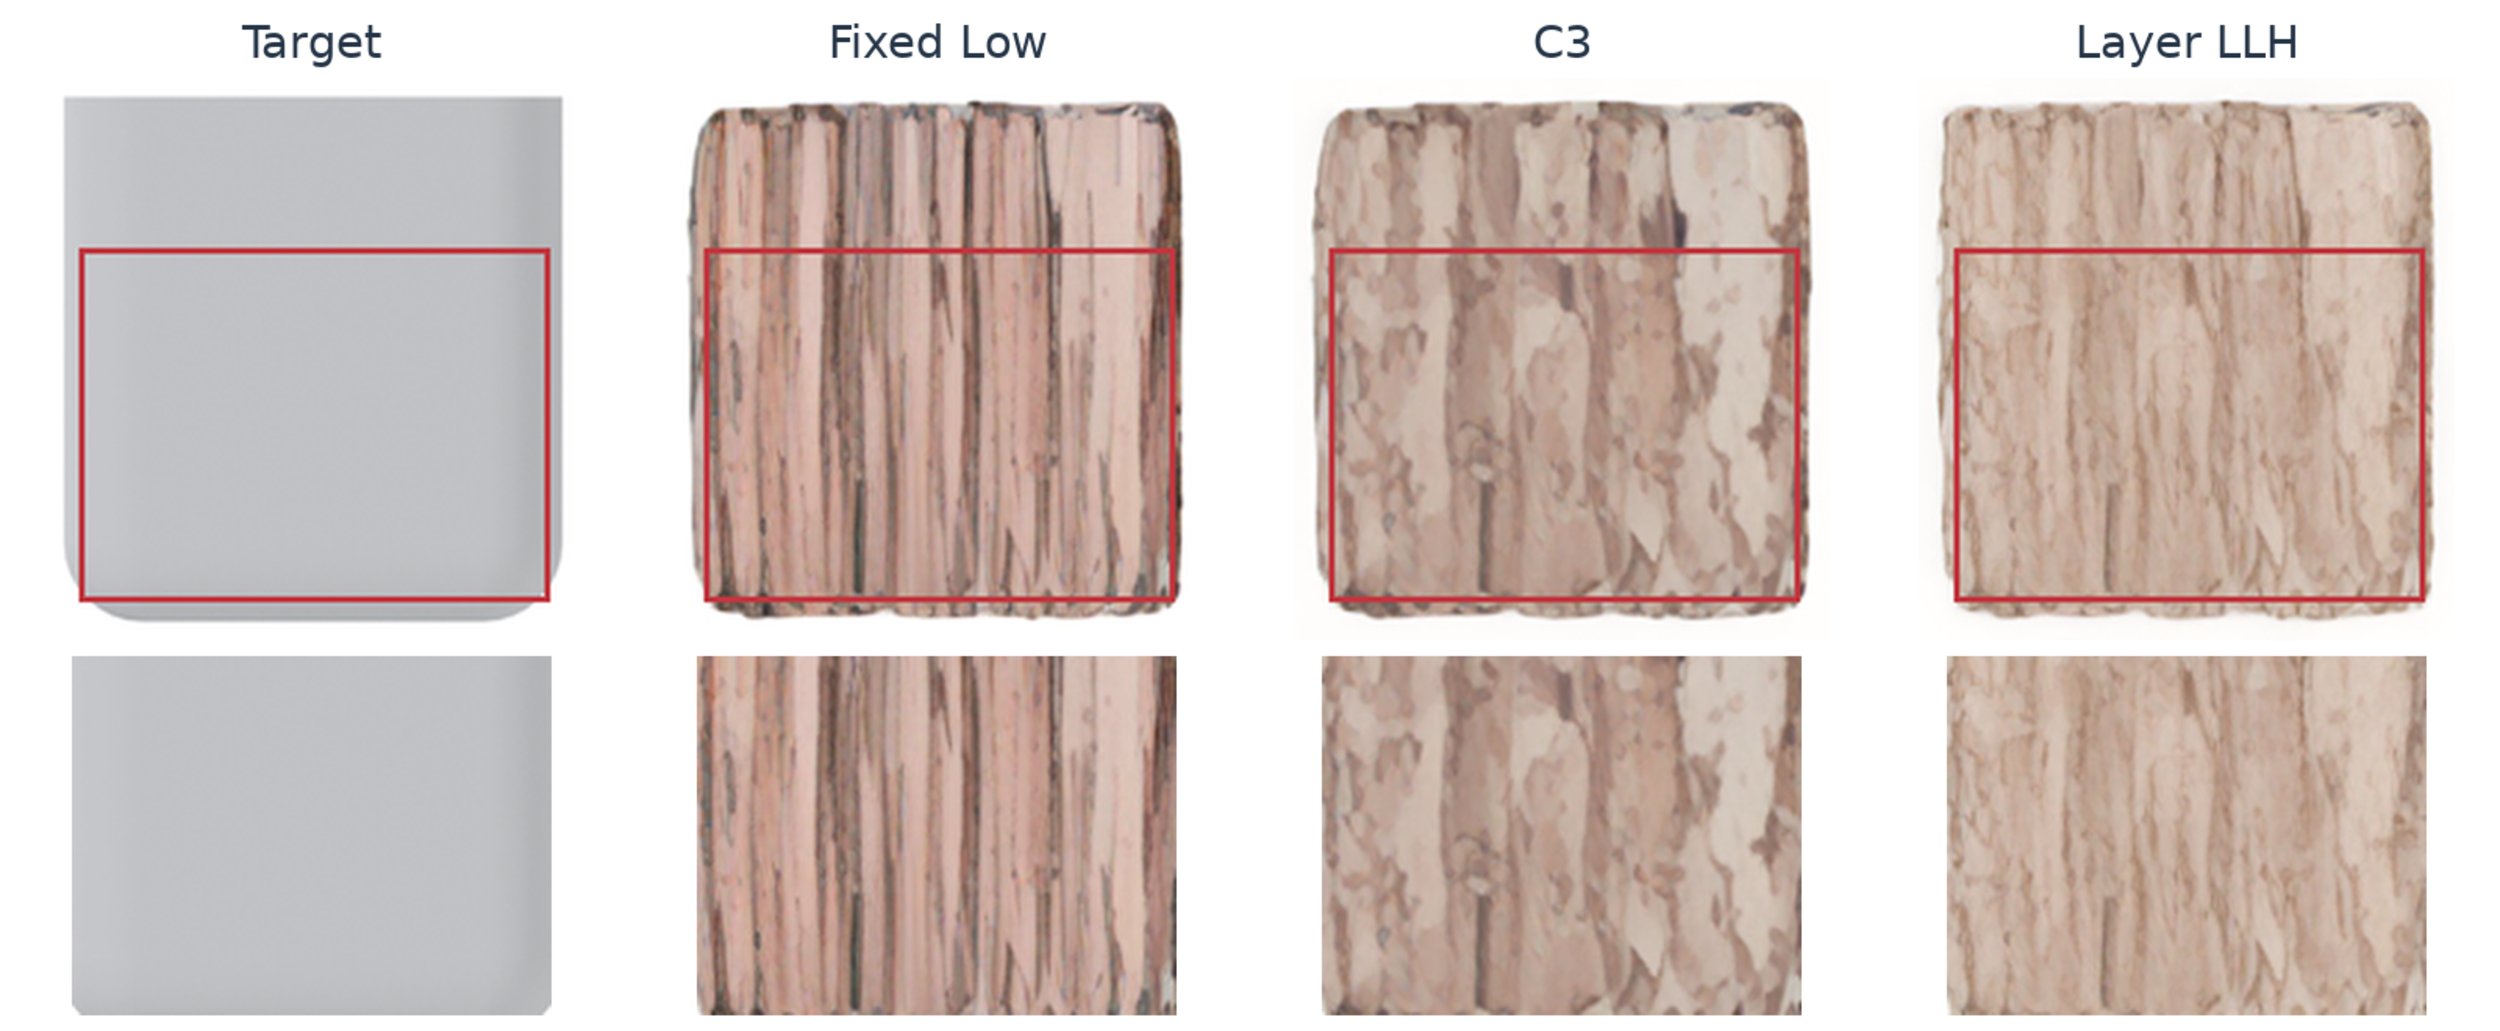
\includegraphics[width=\textwidth]{figures/fig6_color_diagnostic_freshc_context_roi.pdf}
\caption{\DIFaddFL{Fresh C view 0, E5-5-2: target, Fixed Low, C3 and layer LLH share a complete-object frame and an identical pixel crop. The generated brown pattern does not reproduce the gray target; changing its variation does not establish color fidelity. This previously viewed example came from an existing C3--GFL LPIPS stratum and was not selected for color. It does not reproduce the legacy purple-shift cases. The malformed disabled-adapter panel is omitted from this display; its numerical results remain in the full analysis. Source/display identities and attribution are supplied with the final visual manifest and Supplementary Section~S9.}}
\label{fig:color-failure}
\end{figure*}
\DIFaddend 

\DIFdelbegin %DIFDELCMD < \begin{table}[t]
%DIFDELCMD < \centering
%DIFDELCMD < \caption{Uniform adapter scale sweep results.}
%DIFDELCMD < \label{tab:sweep}
%DIFDELCMD < \small
%DIFDELCMD < \begin{tabular}{lcccc}
%DIFDELCMD < \toprule
%DIFDELCMD < Scale & $\Delta$FG-SSIM$\uparrow$ & POS & $\Delta$Crop-SSIM$\uparrow$ & $\Delta$PSNR$\uparrow$ \\
%DIFDELCMD < \midrule
%DIFDELCMD < 0.75 & $-$0.013 & 20/50 & +0.113 & 7.53 \\
%DIFDELCMD < 0.90 & +0.024 & 30/50 & +0.137 & 8.32 \\
%DIFDELCMD < 1.00 & +0.047 & 34/50 & +0.147 & 8.79 \\
%DIFDELCMD < 1.10 & +0.070 & 36/50 & +0.159 & 9.08 \\
%DIFDELCMD < 1.15 & +0.071 & 36/50 & +0.157 & 9.25 \\
%DIFDELCMD < 1.25 & +0.088 & 37/50 & +0.161 & 9.37 \\
%DIFDELCMD < 1.35 & +0.100 & 39/50 & +0.163 & 9.63 \\
%DIFDELCMD < 1.50 & +0.113 & 40/50 & +0.163 & 9.76 \\
%DIFDELCMD < 1.60 & +0.120 & 42/50 & +0.166 & 9.83 \\
%DIFDELCMD < 1.75 & +0.127 & 43/50 & +0.173 & 9.97 \\
%DIFDELCMD < 2.00 & +0.134 & 44/50 & +0.169 & 9.96 \\
%DIFDELCMD < 2.25 & +0.142 & 43/50 & +0.175 & 9.91 \\
%DIFDELCMD < 2.50 & +0.145 & 44/50 & +0.165 & 9.91 \\
%DIFDELCMD < \bottomrule
%DIFDELCMD < \end{tabular}
%DIFDELCMD < \end{table}
%DIFDELCMD < %%%
\DIFdelend \DIFaddbegin \begin{table}[t]
\centering
\scriptsize
\setlength{\tabcolsep}{3pt}
\caption{Selected paired results from the failure-enriched 26-object color diagnosis. Negative CIEDE2000 differences indicate lower reference-color error for the first condition. The set is descriptive and does not estimate population prevalence.}
\label{tab:color-summary}
\begin{tabular}{p{2.3cm}p{3.3cm}p{1.3cm}}
\toprule
Contrast & Mean CIEDE2000 difference [95\% CI] & Objects \\
\midrule
GFL -- No Adapter & $-19.654$ [$-26.370,-13.248$] & 24/26 lower \\
LLH -- GFL & $+3.583$ [$+0.462,+6.712$] & -- \\
\bottomrule
\end{tabular}
\end{table}
\DIFaddend 

\DIFdelbegin \DIFdel{As the scale increases from $s = 0.75$ to $s = 2.50$, $\Delta$FG-SSIM rises from $-$0.013 to +0.145, and the number of objects with positive improvement increases from 20}\DIFdelend \DIFaddbegin \DIFadd{GFL lowered reference-relative CIEDE2000 in 24}\DIFaddend /\DIFaddbegin \DIFadd{26 objects, while visible pink or purple shifts remained in two legacy Fig.~4 cases under No Adapter, GFL, and LLH. Their mapping to the original submitted panels cannot be recovered; the traceable Fresh C example in Figure~\ref{fig:color-failure} is a different object and is not presented as a reproduction of those cases. The decoded RGB output showed the shifts before UV projection or baking, and a late denoising snapshot (update 40 of }\DIFaddend 50\DIFdelbegin \DIFdel{to 44}\DIFdelend \DIFaddbegin \DIFadd{) showed one of them. In that case, a ground-truth VAE encode--decode isolate had CIEDE2000 4.086 and $\Delta a^*\approx-1.35$, compared with 22.032 and $+1.977$ for GFL. This weakens ordinary VAE round-trip error as the sole explanation in that case; it does not identify the complete cause or rule out other model and conditioning effects.
}

\DIFadd{LLH--GFL increased mean CIEDE2000 while reducing foreground gradient magnitude, high-frequency energy and color entropy. Lower variation therefore did not imply closer reference appearance. The denoising}\DIFaddend /\DIFdelbegin \DIFdel{50. This indicates that stronger adapter residuals indeed improve the model's adherence to geometric conditions such as normals, depth maps, and foreground contours.
Figure~\textit{[removed reference: }\texttt{fig:curve}\textit{]} visualizes this trend: FG-SSIM keeps increasing with adapter scale, while Crop-SSIM saturates and slightly decreases at high scales}\DIFdelend \DIFaddbegin \DIFadd{runtime isolates and three failed correction candidates remain in Supplementary Section~S6; they localize observations but do not validate a cause or repair}\DIFaddend .

\DIFdelbegin %DIFDELCMD < \begin{figure}[t]
%DIFDELCMD < \centering
%DIFDELCMD < 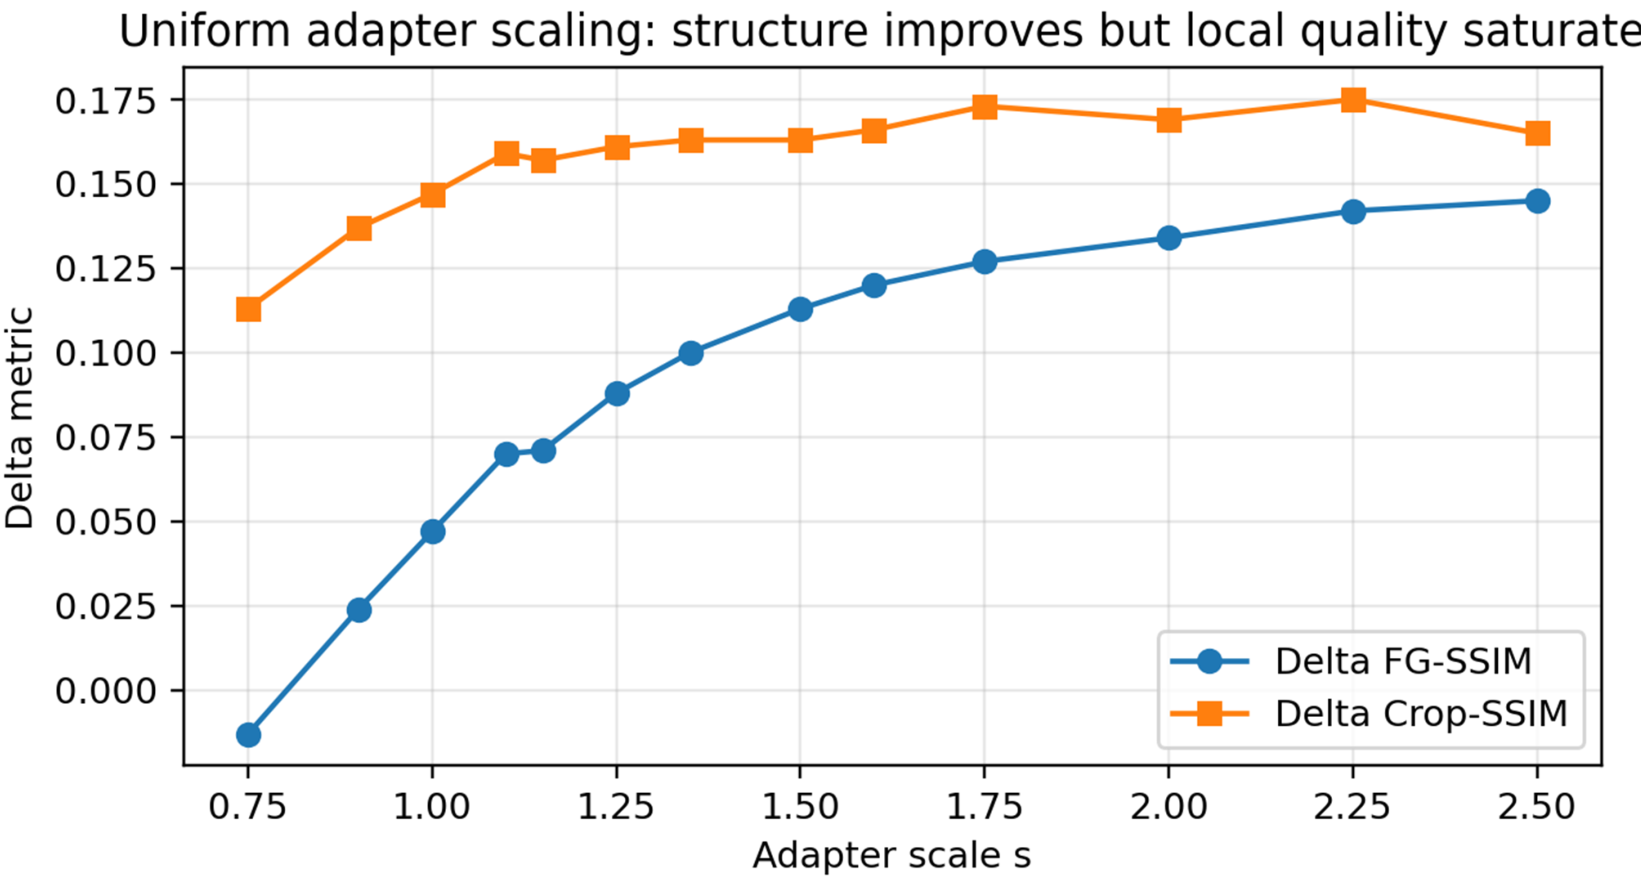
\includegraphics[width=\columnwidth]{fig2.pdf}
%DIFDELCMD < %%%
%DIFDELCMD < \caption{%
{%DIFAUXCMD
\DIFdelFL{Structural metric changes under uniform adapter scaling. The curves show that FG-SSIM keeps increasing with adapter scale, while Crop-SSIM saturates and slightly decreases at high scales. Stronger geometric control therefore mainly improves structural alignment, but does not necessarily keep improving local foreground quality.}}
%DIFAUXCMD
%DIFDELCMD < \label{fig:curve}
%DIFDELCMD < \end{figure}
%DIFDELCMD < %%%
\DIFdelend \DIFaddbegin \DIFadd{Historical twenty-object results, the earlier five-object bake, invalidated camera/mask attempts and the corrected REPEAT sampler are reported separately in Supplementary Section~S5. They are not pooled with the new ten-object cohort. The actual unset-scale GeoTex residual branch differs from Constant 1.0 (capped), so the latter is not labeled an unmodified pipeline.
}\DIFaddend 

\DIFdelbegin \DIFdel{Overall, the FG-SSIM improvement is stable, but the marginal benefit becomes smaller in }\DIFdelend \DIFaddbegin \paragraph{Full-object evidence and its selection.}
\DIFadd{The strong-fixed and Generic Linear examples in Figure~\ref{fig:c3compare} and }\DIFaddend the \DIFdelbegin \DIFdel{high-scale region. For example, increasing the scale from $s = 2.25$ to $s = 2.50$ yields only a limited FG-SSIM gain, while Crop-SSIM already decreases. This suggests that the nature of the high-scale benefit may change: the gain comes more from contour smoothing and foreground alignment than from preservation of local texture details. Figure~\textit{[removed reference: }\texttt{fig:heatmap}\textit{]} shows the per-object $\Delta$FG-SSIM heatmap, confirming that most objects gain higher structural scores as the scale increases, but with clear object-level differences}\DIFdelend \DIFaddbegin \DIFadd{color failure in Figure~\ref{fig:color-failure} use common framing and exact shared pixel crops. Favorable/adverse C3--GFL examples are retained in Supplementary Section~S9}\DIFaddend . \DIFdelbegin %DIFDELCMD < 

%DIFDELCMD < \begin{figure}[t]
%DIFDELCMD < \centering
%DIFDELCMD < 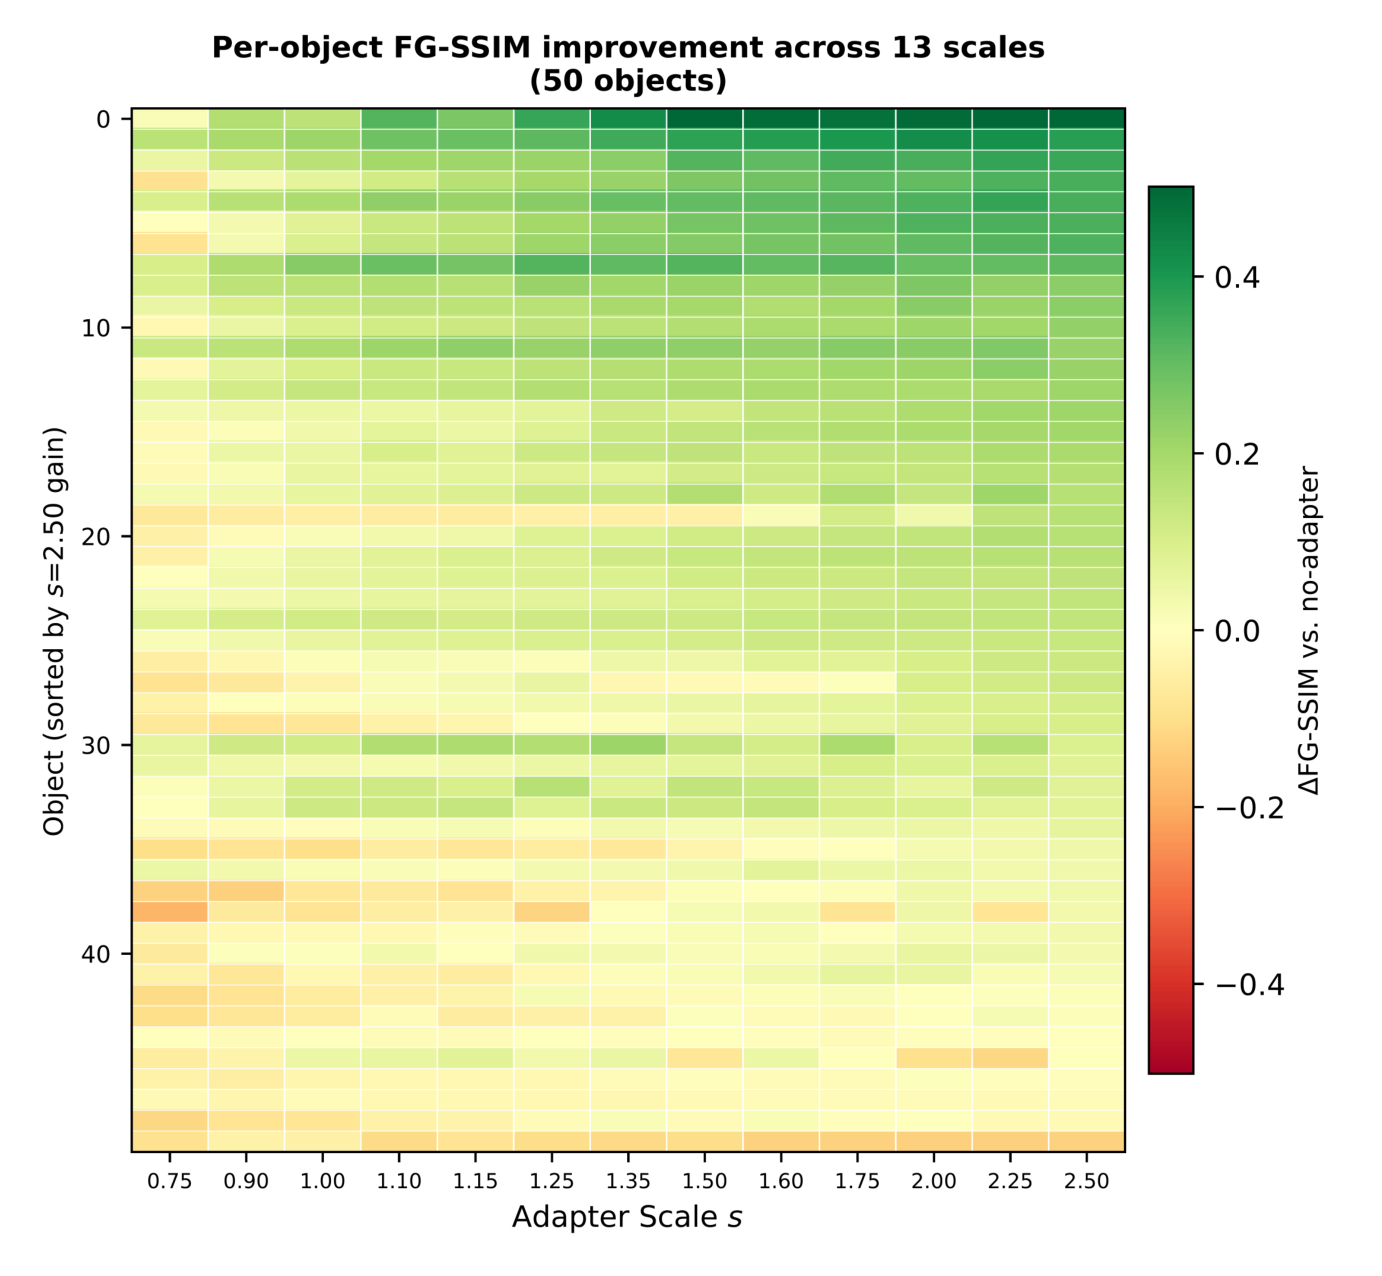
\includegraphics[width=\columnwidth]{fig3.pdf}
%DIFDELCMD < %%%
%DIFDELCMD < \caption{%
{%DIFAUXCMD
\DIFdelFL{$\Delta$FG-SSIM heatmap for 50 objects under 13 adapter scales. Most objects obtain higher structural gains as the scale increases, but there are clear object-level differences.}}
%DIFAUXCMD
%DIFDELCMD < \label{fig:heatmap}
%DIFDELCMD < \end{figure}
%DIFDELCMD < 

%DIFDELCMD < \subsection{Texture Audit: High Scale Causes Texture Flattening}
%DIFDELCMD < \label{subsec:audit}
%DIFDELCMD < 

%DIFDELCMD < %%%
\DIFdel{To determine whether the FG-SSIM gain at high scales reflects better visual quality, we further conduct a texture audit on 26 objects, comparing texture metrics and foreground shape changes for $s = 2.50$ relative to $s = 1.25$. Figure~\textit{[removed reference: }\texttt{fig:qualitative}\textit{]} should be read as a local texture comparison rather than as a claim that any method fully matches the ground truth: the key evidence is the progressive loss of color variation, material marks, and high-frequency patterns inside the marked regions as the scale increases. The conservative scale $s = 1.25$ better preserves color variation and local texture, while $s = 2.50$ more easily produces uniform and smooth surfaces. }%DIFDELCMD < 

%DIFDELCMD < \begin{figure}[!t]
%DIFDELCMD < \centering
%DIFDELCMD < \includegraphics[width=\columnwidth]{fig4.pdf}
%DIFDELCMD < %%%
%DIFDELCMD < \caption{%
{%DIFAUXCMD
\DIFdelFL{Texture degradation under different adapter scales. Each row shows one object; large crops highlight local texture regions (thumbnails below indicate crop locations). Green borders denote conservative scaling $s = 1.25$; red borders denote aggressive scaling $s = 2.50$. Within each row, increasing the adapter scale causes progressive loss of color variation and high-frequency detail: surfaces become more uniform and color-saturated, indicating that stronger geometric correction suppresses the base model's texture synthesis capability.}}
%DIFAUXCMD
%DIFDELCMD < \label{fig:qualitative}
%DIFDELCMD < \end{figure}
%DIFDELCMD < 

%DIFDELCMD < %%%
\DIFdel{The results show that 24 out of 26 objects (}\DIFdelend \DIFaddbegin \DIFadd{Outcome-selected displays illustrate behavior, not prevalence. The unrecoverable historical texture audit's }\DIFaddend 92\% \DIFdelbegin \DIFdel{) exhibit a pattern of ``texture loss without true shape gain.
'' Only two objects show comparable texture quality, and no object shows a clear texture improvement from the high scale. Here, ``true shape gain'' is not equivalent to an increase in FG-SSIM. It refers to whether the high scale brings substantive improvement in effective foreground area, contour structure, or geometric detail compared with the conservative scale. If the metric improvement mainly comes from smoothed foreground boundaries or averaged contour errors without visible geometric improvement, it is categorized as having no true shape gain. Therefore, although a high adapter scale can improve structural metrics, such improvement does not necessarily indicate better visual shape or texture quality. Figure~\textit{[removed reference: }\texttt{fig:audit}\textit{]} further quantifies this texture loss.
}%DIFDELCMD < 

%DIFDELCMD < \begin{figure}[t]
%DIFDELCMD < \centering
%DIFDELCMD < \includegraphics[width=\columnwidth]{fig5.pdf}
%DIFDELCMD < %%%
%DIFDELCMD < \caption{%
{%DIFAUXCMD
\DIFdelFL{Texture flattening at $s = 2.50$. Top: RGB standard deviation ratio on 26 objects ($s = 2.50$ / $s = 1.25$). Bottom: gradient magnitude ratio. Values below 1.0 indicate texture loss. Even the eight best-improvement objects (green) show 18\% to 30\% texture loss despite positive FG-SSIM gains.}}
%DIFAUXCMD
%DIFDELCMD < \label{fig:audit}
%DIFDELCMD < \end{figure}
%DIFDELCMD < 

%DIFDELCMD < %%%
\DIFdel{For multi-view texture generation, overly strong geometric control can suppress the color and detail synthesis capability of the base diffusion model during late denoising steps, making surfaces more uniform. Therefore, scale selection should not rely only on standard metrics such as FG-SSIM or PSNR, but should also incorporate texture-sensitive diagnostics. }%DIFDELCMD < 

%DIFDELCMD < \subsection{Timestep-Conditioned Adapter Scaling: Shape-Texture Balance of C3}
%DIFDELCMD < \label{subsec:c3}
%DIFDELCMD < %%%
\DIFdelend \DIFaddbegin \DIFadd{prevalence claim and its texture-loss classifications are withdrawn; variation statistics alone would not validate fidelity even if their lineage were complete.
}\DIFaddend 


\DIFdelbegin \DIFdel{Based on the texture audit, we do not pursue higher adapter scales throughout the entire denoising process. Instead, we further explore how different scaling strategies balance shape gain and texture loss. We construct 17 adapter scaling variants and evaluate them on the 24-object probe set. To avoid turning the 300-object evaluation pool into a hyperparameter search, the schedule selected in this probe stage is frozen before large-scale evaluation. These variants include three categories: uniform scaling baselines, layer-wise scaling strategies, }\DIFdelend \DIFaddbegin \subsection{Actual Baked Appearance: Local Benefit and External Limits}
\label{subsec:new-bake}
\DIFadd{We froze ten previously unbaked Fresh C objects in UID order using input availability, native UV/material compatibility, triangle-count }\DIFaddend and \DIFdelbegin \DIFdel{timestep-conditioned scaling strategies.
Uniform scaling tests the effect of globally strengthening adapter influence and serves as the closest counterpart to using a single ControlNet-style condition scale. Layer-wise scaling examines whether redistributing the same geometric intervention across UNet levels is sufficient. Timestep scaling tests stage placement directly, including variants that put high adapter strength in early, middle, late, or broader temporal regions. This design is intended to rule out the simple explanation that any guidance-like schedule or any stronger controlscale would solve the problem. }\DIFdelend \DIFaddbegin \DIFadd{camera-mask alignment criteria. Of the 300 screened inputs, only ten passed all criteria before the cutoff; the planned maximum was twenty. The ten are not new to the GeoTex image domain, but their baked outcomes had not been inspected during selection. This is a compatibility-selected pilot, not a representative twenty-object confirmation. Five earlier bake objects are reported separately.
}\DIFaddend 

\DIFdelbegin \DIFdel{All variants are evaluated using $\Delta$FG-SSIM for shape gain and $\Delta$Lap Var for texture detail change. Delta texture metrics are computed relative to the corresponding ground-truth foreground renderings under the same views and masks. Importantly, the objective of this probe experiment is not to find the single highest structural score,but to identify a stable compromise strategy that avoids the trap of ``higher structural metrics but flattened texture. '' This criterion is crucial: if a schedule improves FG-SSIM by applying strong geometry residuals late but causes a clear drop in texture response, then it does not solve the adapter-specific conflict even though it appears favorable under a structure-only metric. }\DIFdelend \DIFaddbegin \DIFadd{Seven conditions share each object's source mesh, reference, seed, six projection cameras, masks, 256-pixel source resolution, atlas resolution, hole filling and eleven unseen evaluation cameras. Original geometry, UVs and legal base-color material semantics are retained and checked. Unseen cameras do not enter the bake. GT-256 uses the same source resolution, masks and bake parameters and has exactly the same raw atlas coverage as every generated condition. The separately tested CPU REPEAT sampler passes boundary and integer-period tests; it is not the sampler used by this GPU bake. Pole-view RGB orientation is corrected without rotating raw-camera masks. These calibrations control projection artifacts; evaluation is unlit base color, not PBR fidelity. Supplementary Section~S5 records the checks and object-level data.
}\DIFaddend 

\DIFdelbegin %DIFDELCMD < \begin{table}[t]
%DIFDELCMD < \centering
%DIFDELCMD < \caption{Shape-texture trade-off on the 24-object probe set. Delta texture metrics are computed relative to the corresponding ground-truth foreground renderings under the same views and masks; $\Delta$Lap Var closer to 0 indicates smaller texture loss. Eight representative variants of the 17 evaluated are shown; the complete set is visualized in Fig.~\textit{[removed reference: }\texttt{fig:pareto}\textit{]}.}
%DIFDELCMD < \label{tab:probe}
%DIFDELCMD < \footnotesize\setlength{\tabcolsep}{3pt}
%DIFDELCMD < \begin{tabular}{llccc}
%DIFDELCMD < \toprule
%DIFDELCMD < Variant & Category & $\Delta$FG-SSIM$\uparrow$ & $\Delta$Lap Var $\to$ 0 & Assessment \\
%DIFDELCMD < \midrule
%DIFDELCMD < C4 & Late-stage high & 0.105 & $-$0.0120 & Trap \\
%DIFDELCMD < C2 & Timestep sched. & 0.104 & $-$0.0110 & Trap \\
%DIFDELCMD < B2 & Layer-wise sched. & 0.090 & $-$0.0135 & Trap \\
%DIFDELCMD < A\_s2.00 & Uniform & 0.087 & $-$0.0062 & Trap \\
%DIFDELCMD < C3 (TCAS) & Mid-stage high & 0.084 & $-$0.0006 & Promising \\
%DIFDELCMD < A\_s2.25 & Uniform & 0.079 & $-$0.0096 & Trap \\
%DIFDELCMD < A\_s2.50 & Uniform & 0.078 & $-$0.0108 & Trap \\
%DIFDELCMD < B6 & Layer-wise sched. & 0.000 & $-$0.0027 & OK \\
%DIFDELCMD < \bottomrule
%DIFDELCMD < \end{tabular}
%DIFDELCMD < \end{table}
%DIFDELCMD < %%%
\DIFdelend \DIFaddbegin \begin{table}[ht]
\centering\scriptsize
\caption{New ten-object unlit unseen-view bake pilot. Eleven views are averaged per object. Higher PSNR/SSIM and lower LPIPS/CIEDE2000 are favorable. Constant 1.0 is an explicitly capped request, not the unset-scale pipeline. All seven original generated conditions and all ten eligible objects are retained; the two subsequently added controls marked $\dagger$ are exploratory; GT-256 is a separate matched reference bake, not a theoretical bound.}
\label{tab:new-bake}
\begin{tabular}{lrrrr}
\toprule Condition & FG-PSNR & FG-LPIPS & FG-SSIM & CIEDE2000 \\
\midrule
GT-256 reference bake & 22.38 & 0.0590 & 0.7683 & 4.44 \\
\midrule
Native residual$^\dagger$ & 11.13 & 0.1372 & 0.3376 & 26.47 \\
No Adapter$^\dagger$ & 5.92 & 0.1600 & 0.3829 & 40.92 \\
Constant 1.0 (capped) & 11.93 & 0.1354 & 0.3504 & 24.18 \\
Fixed Low & 12.48 & 0.1317 & 0.3835 & 22.71 \\
Fixed High & 12.29 & 0.1305 & 0.4587 & 23.27 \\
Fixed Mean & 12.62 & 0.1303 & 0.4193 & 22.32 \\
C3 / Middle-high & 12.48 & 0.1302 & 0.4059 & 22.16 \\
Late-high & 12.92 & 0.1277 & 0.4259 & 21.65 \\
Generic Linear & 11.60 & 0.1276 & 0.4458 & 24.71 \\
\bottomrule\end{tabular}
\end{table}
\DIFaddend 

\DIFdelbegin \DIFdel{Table~\textit{[removed reference: }\texttt{tab:probe}\textit{]} summarizes representative scheduling variants on the 24-object probe set. C4 and other late-stage high-scale strategies obtain higher $\Delta$FG-SSIM, but they are accompanied by obvious decreases in Laplacian variance, indicating that their structural gains come at the cost of texture loss. This is the main reason a direct transfer of guidance scheduling intuition is insufficient: a schedule can make the condition stronger at apparently useful timesteps and still damage the texture signal that matters for 3D appearance. Uniform high-scale strategies show a similar problem. For example, $s = 2.50$ achieves $\Delta$FG-SSIM of +0.078, but $\Delta$Lap Var decreases to $-$0.0108.
In contrast, }\DIFdelend \DIFaddbegin \DIFadd{The internally predeclared primary contrast was Late-high minus Fixed Mean on unseen-view FG-LPIPS, proposed from the earlier pilot and tested on the ten newly selected bake objects. Its mean is $-0.00265$ (95\% object-bootstrap CI $[-0.00414,-0.00137]$; exact paired sign-flip $p=0.00195$), with all ten objects favorable. This is approximately a 2.0\% reduction relative to Fixed Mean's mean LPIPS, and identifies a small allocation benefit within this sampling protocol. Generic Linear has a slightly lower mean LPIPS but lower PSNR; Late-high does not dominate every endpoint or control. The matched GT-256 reference bake has mean LPIPS 0.0590, versus 0.1303 for Fixed Mean and 0.1277 for Late-high. A post hoc description therefore puts the absolute gain in context: it closes only 3.7\% of the mean Fixed Mean--GT reference gap (pointwise object-bootstrap CI }[\DIFadd{2.3\%,5.3\%}]\DIFadd{). This ratio of paired means is not a theoretical ceiling, a new primary test or evidence of acceptable material fidelity. Leaving out each object in turn keeps the mean Late--Mean difference between $-0.00294$ and $-0.00208$, but all substantial reference-appearance discrepancies remain. Supplementary Section~S5 supplies the paired values and calculation.
}

\DIFadd{C3--Fixed High has mean PSNR $+0.19$~dB (95\% CI $[-0.65,+0.87]$) and LPIPS $-0.00036$ ($[-0.00396,+0.00336]$); neither separates under the four-comparison secondary Holm family (both adjusted $p=1$). Its SSIM is lower by 0.05274 ($[-0.07459,-0.03170]$; Holm $p=0.00781$). Thus the old five-object }\DIFaddend C3 \DIFdelbegin \DIFdel{achieves $\Delta$FG-SSIM of +0.084. Although it is slightly lower than some aggressive variants in structure gain, its Laplacian variance loss is only $-$0.0006, close to zero texture loss. Therefore, }\DIFdelend \DIFaddbegin \DIFadd{PSNR advantage does not repeat stably on this new pilot. We retain }\DIFaddend C3 \DIFdelbegin \DIFdel{is the only variant labeled Promising. We freeze this configuration before large-scale evaluation }\DIFdelend \DIFaddbegin \DIFadd{as the historical candidate }\DIFaddend and do not \DIFdelbegin \DIFdel{tune it on the 300-object set.
}%DIFDELCMD < 

%DIFDELCMD < %%%
\DIFdel{The specific configuration of C3 uses the conservative scale $s = 1.25$ in the early and late stages, and the strong scale $s = 2.50$ in the middle geometry-refinement stage, i.e. , }\DIFdelend \DIFaddbegin \DIFadd{rename Late-high as }\DIFaddend C3\DIFdelbegin \DIFdel{= (1.25, 2.50, 1.25). Its motivation follows the staged role of diffusion denoising. In the early stage, latent variables are still highly noisy, and strong geometric correction can interfere with global structure formation. In the middle stage, the signal becomes more stable, making it suitable to strengthen geometric constraints such as normals, depth maps, and foreground contours. In the late stage, generation mainly focuses on color, material , and fine texture synthesis, so adapter intervention should be reduced to preserve the texture generation space of the base diffusion model}\DIFdelend .

\DIFdelbegin \DIFdel{Figure~\ref{fig:c3compare} provides a qualitative comparison between C3 and uniform adapter scaling. The red-boxed zoom-in regions make the intended comparison visible: conservative scaling preserves more color variation but provides weaker structural correction,whereas aggressive scaling strengthens geometric constraints but flattens surface texture. C3 applies strong geometric correction in the middle stage and reduces adapter intervention in the late stage, thereby preserving more local texture than $s = 2.50$ while retaining stronger geometric correction than the conservative scale}\DIFdelend \DIFaddbegin \DIFadd{Across the seven conditions, mean within-object Spearman correlations between generated-view and baked unseen-view rankings are 0.846 for PSNR, 0.804 for LPIPS, 0.746 for SSIM and 0.907 for Edge-SSIM. Broad rankings are positively associated, while the winning condition changes on 7/10 objects for LPIPS (1/10 for PSNR). These are different statements: we do not claim a general reversal of rankings. Full-object Figure~\ref{fig:baked-context} also shows persistent appearance errors, including the Tire's brown output against a gray reference. A lower LPIPS does not establish faithful material reproduction}\DIFaddend .

\DIFdelbegin %DIFDELCMD < \begin{figure}[!t]
%DIFDELCMD < %%%
\DIFdelendFL \DIFaddbeginFL \begin{figure*}[t]
\DIFaddendFL \centering
\DIFdelbeginFL %DIFDELCMD < \includegraphics[width=\columnwidth]{fig6.pdf}
%DIFDELCMD < %%%
%DIFDELCMD < \caption{%
{%DIFAUXCMD
\DIFdelFL{Qualitative comparison between C3 and uniform adapter scaling. Large crops show local texture regions (thumbnails below indicate crop locations). Columns: GT (gray), $s = 1.25$ (green), $s = 2.50$ (red), and C3 (orange). Compared with $s = 2.50$, C3 retains more local color variation and material texture while preserving stronger geometric correction than the conservative scale.}}
%DIFAUXCMD
%DIFDELCMD < \label{fig:c3compare}
%DIFDELCMD < \end{figure}
%DIFDELCMD < %%%
\DIFdelend \DIFaddbegin 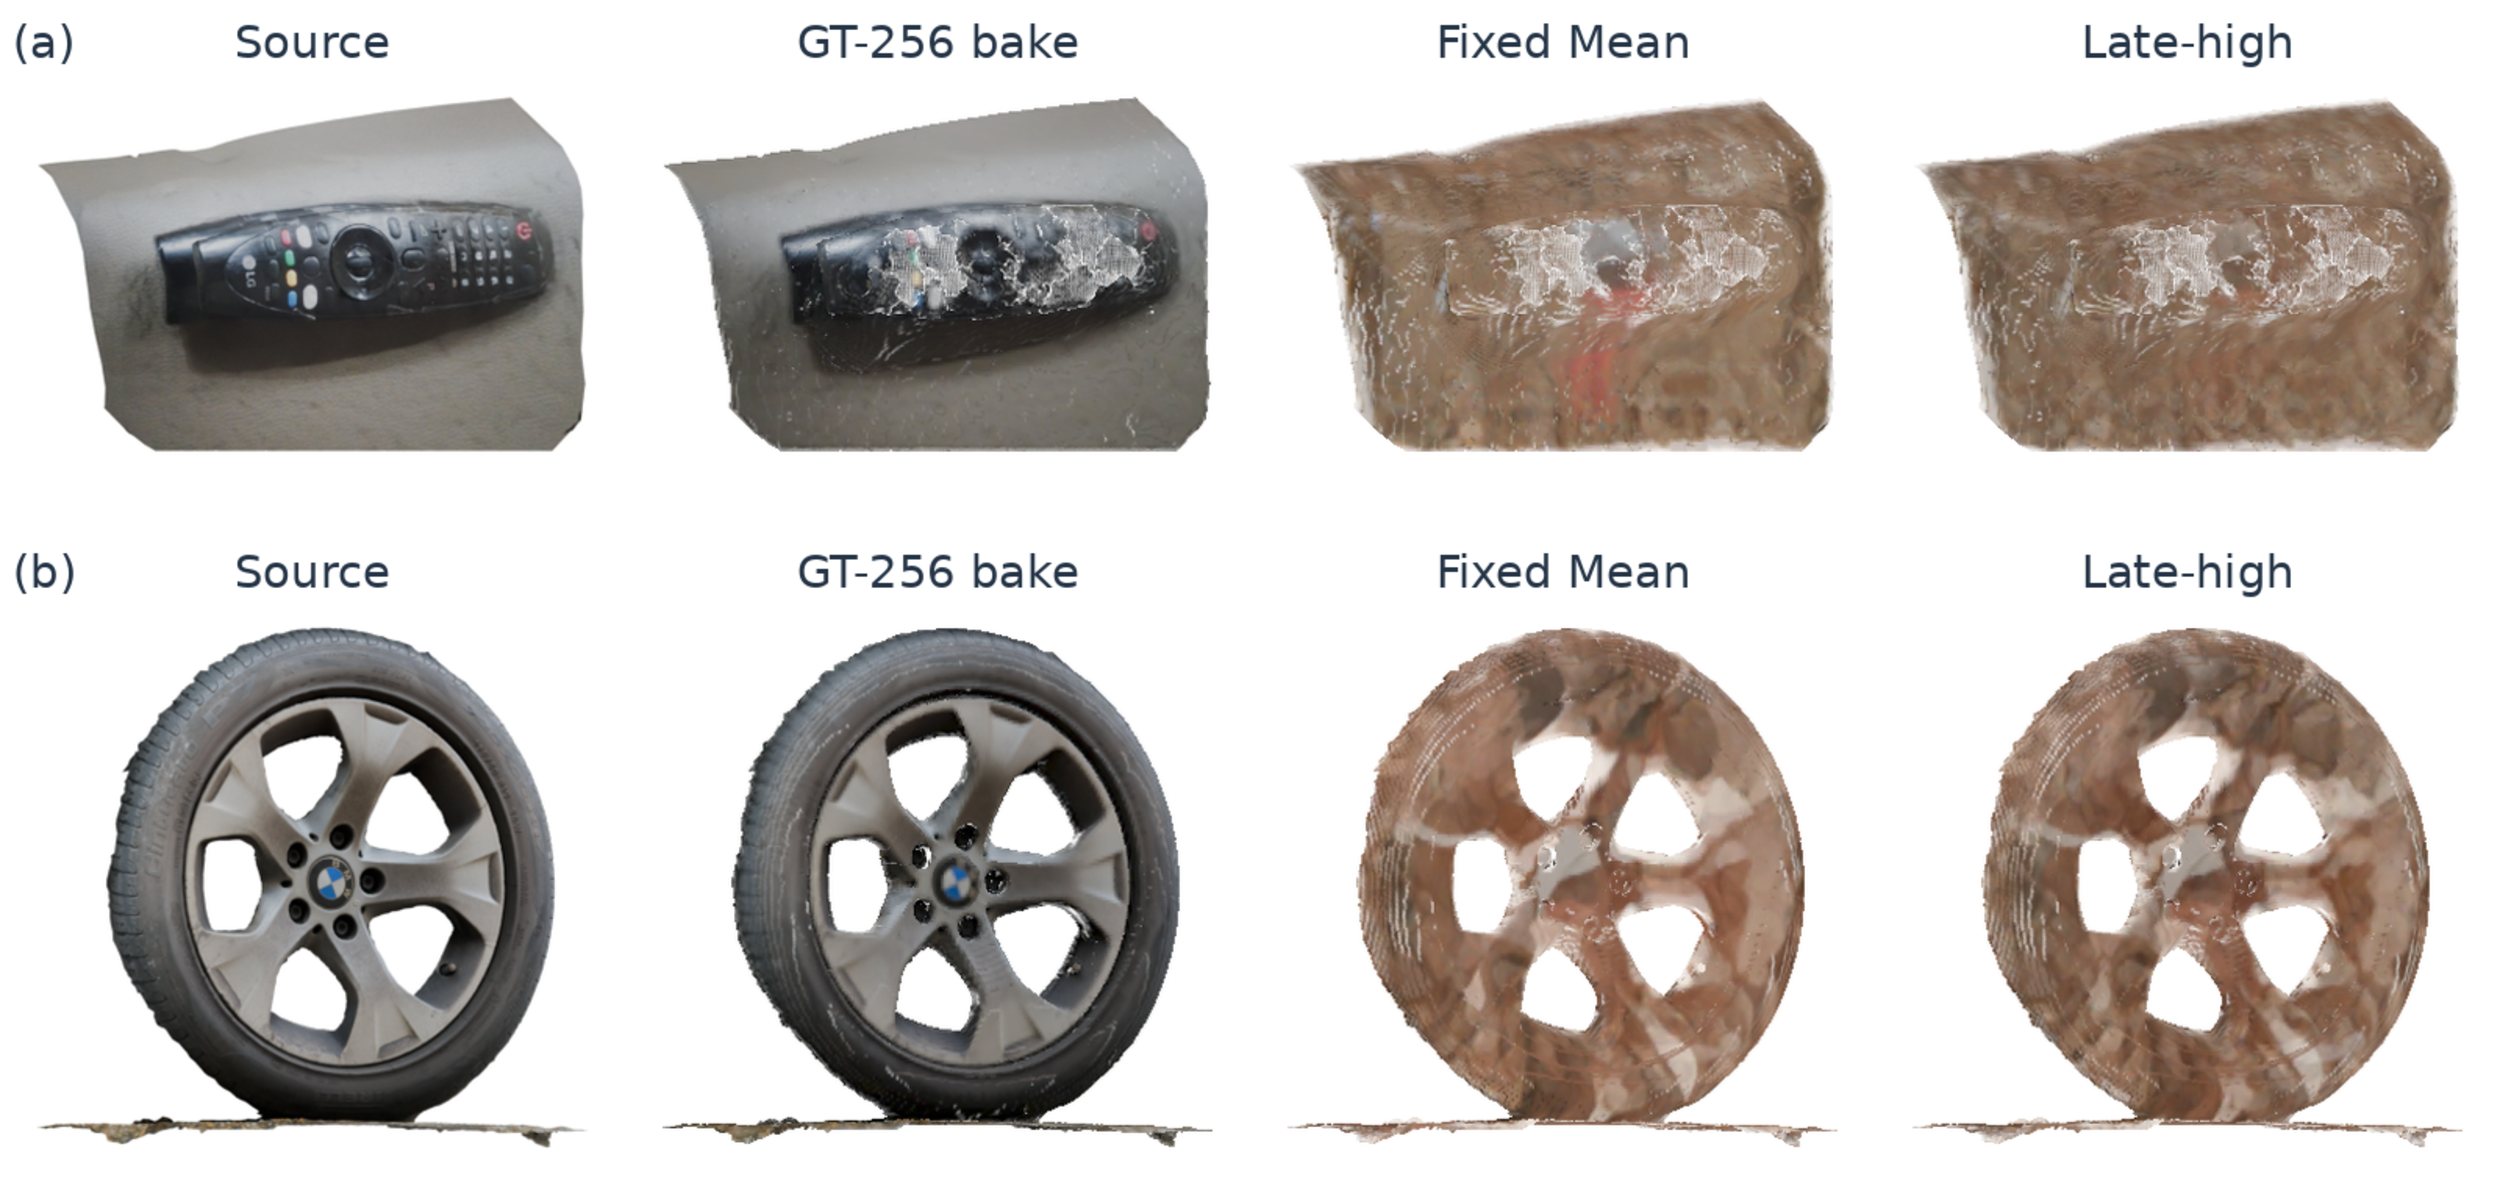
\includegraphics[width=\textwidth]{figures/fig8_baked_unseen_context.pdf}
\caption{\DIFadd{Unseen camera 004: (a) LG Remote and (b) Tire. Source and matched GT-256 bake separate projection loss from generated appearance; Fixed Mean and Late-high show the specified allocation comparison. Columns share a full-object frame determined from source, GT and every original condition, without color or detail editing. These are the first two input-order objects with verified publication licenses, not quality-selected examples. Persistent brown-pattern and material errors remain visible. Complete seven-condition displays for all seven rights-cleared objects are in Supplementary Section~S5; all ten objects enter the numerical analysis. Credits: mohd.akmal.mahyudin and Koto3D Stephane Vogley, CC Attribution (full source links in Supplementary Section~S5).}}
\label{fig:baked-context}
\end{figure*}
\DIFaddend 


\DIFdelbegin \DIFdel{Figure~\textit{[removed reference: }\texttt{fig:pareto}\textit{]} further shows the distribution of the 17 variants in the shape-texture space. Most variants with high shape gain are accompanied by large texture loss and fall into the Trap region, whereas C3 maintains a relatively high shape gain while keeping texture loss near zero. Thus, the value of C3 is not that it maximizes every metric, but that it avoids the trap of ``higher structural scores but flattened texture, '' resulting in a more stable shape-texture compromise}\DIFdelend \DIFaddbegin \paragraph{Separate twenty-object GSO evaluation.}
\DIFadd{The GSO/MV-Adapter study completes twelve conditions by three seeds on twenty fixed inputs, plus twenty matched GT self-bakes: 740 unique baked meshes and 8,140 unseen-view records. The objects, source meshes, projection cameras, texture resolution and eleven unseen cameras are shared across controls; unseen cameras do not contribute to baking}\DIFaddend .

\DIFdelbegin %DIFDELCMD < \begin{figure}[!t]
%DIFDELCMD < \centering
%DIFDELCMD < \includegraphics[width=\columnwidth]{fig7.pdf}
%DIFDELCMD < %%%
%DIFDELCMD < \caption{%
{%DIFAUXCMD
\DIFdelFL{Shape-texture Pareto trade-off among 17 variants. The horizontal axis is shape gain, where farther right is better; the vertical axis is the Laplacian-variance change, where higher (closer to zero) is better; therefore, the top-right region represents a more desirable compromise. C3 (star) lies in the Promising region, with high shape gain and nearly zero texture loss. Most high-shape-gain variants fall into the Trap region, where structural scores are obtained at the cost of large texture loss. Variants such as B1 have smaller texture degradation but almost no shape gain.}}
%DIFAUXCMD
%DIFDELCMD < \label{fig:pareto}
%DIFDELCMD < \end{figure}
%DIFDELCMD < %%%
\DIFdelend \DIFaddbegin \DIFadd{The original attempt stopped after fifteen objects because a discontinuous UV-ramp diagnostic failed on a Hair Dryer. Subsequent GT-only tests identify finite-resolution mixing across UV jumps and validate continuous nonlinear surface-color fields, an independent multi-island analytic fixture, and a deliberate image-flip negative control. The resulting calibration addendum is post hoc. It keeps projection, masks, cameras, material semantics, resolutions and the fixed twenty objects unchanged; all 375 original GLB hashes and metric records reproduce exactly. The original failure and remaining UV/coverage limitations are retained in Supplementary Section~S4.
}\DIFaddend 

\DIFdelbegin \DIFdel{Mechanistically, the advantage of C3 is not simply the result of hyperparameter tuning; it comes from the functional alignment between adapter correction and the diffusion process's stage-dependent objective. A natural hypothesis might be that correction should be strongest where the correction-to-noise ratio is highest. However, under the Euler sigma schedule, this ratio increases monotonically throughout denoising (from approximately 8 at full noise to over 400 near completion), which would predict that late-stage correction is most effective---a prediction inconsistent with the scheduling-variant results. The correct explanation involves \emph{functional alignment} rather than signal-to-noise ratio.
The adapter correction is derived from geometric conditions(normals, depth, contours) and is therefore constructive only when the diffusion process is actively refining geometric structure. In the early stage ($\sigma > 5$), global structure has not yet emerged, so the correction has no stable target to reinforce and instead disrupts layout formation. In the middle stage ($\sigma \approx 5$--$1.2$), coarse structure is established and the denoiser is performing geometric refinement---the adapter correction direction aligns with this objective, making it maximally constructive. In the late stage ($\sigma < 1.2$), generation shifts to color, material, and fine texture synthesis; geometric correction is orthogonal to this objective and competes with the texture formation process. C3's low-high-low schedule therefore allocates strong correction proportional to functional alignment, not to signal clarity. Notably, this allocation is the reverse of limited-interval CFG guidance \cite{kynkanniemi2024limited}: under adapter residual injection, geometric correction must also be withdrawn near the end of sampling, because the late-stage risk is competition with texture synthesis rather than diversity loss. The schedule is tied to the denoising process's functional role at each stage rather than to validation-set-specific tuning or a generic monotonic guidance rule. }\DIFdelend \DIFaddbegin \DIFadd{Late-high minus Fixed Mean unseen-view LPIPS is $+0.000084$ (pointwise interval $[-0.000103,+0.000286]$; original comparison-family Holm $p=0.788$). This study does not detect the ten-object pilot's benefit. It changes both input domain and conditioning/projection protocol, so it is neither a direct same-protocol replication nor evidence assigning the difference to backbone alone. Table~\ref{tab:bake-cohorts} presents both application comparisons.
}\DIFaddend 

\DIFdelbegin \DIFdel{This explanation is consistent }\DIFdelend \DIFaddbegin \begin{table*}[t]\centering\scriptsize\setlength{\tabcolsep}{4pt}
\caption{Late-high minus Fixed Mean on unseen-view foreground LPIPS. Lower is favorable. All views/seeds are nested within object. The ten-object specified primary uses its original exact sign-flip test; GSO uses the original Holm16 comparison family. Pointwise intervals are not simultaneous. The two cohorts and protocols are not pooled.}
\label{tab:bake-cohorts}
\begin{tabular}{lrrrrl}
\toprule Study & Objects & Fixed Mean & Late-high & Paired difference [95\% CI] & Test \\
\midrule
GeoTex compatibility pilot & 10 & 0.1303 & 0.1277 & $-0.002652\ [-0.004144,-0.001367]$ & exact $p=0.00195$ \\
GSO revised-calibration study & 20 & 0.10089 & 0.10098 & $+0.000084\ [-0.000103,+0.000286]$ & Holm $p=0.788$ \\
\bottomrule\end{tabular}\end{table*}

\DIFadd{Across all twelve GSO conditions, mean within-object image/bake LPIPS-rank correlation is 0.601 (object interval $[0.440,0.733]$). A post hoc sensitivity restricted to the seven original scale/time controls gives 0.396 ($[0.175,0.582]$), }\DIFaddend with the \DIFdelbegin \DIFdel{scheduling-variant results. Early high-scale or early-and-late high-scale variants provide limited structural gain, indicating that early strong intervention is unstable. }\DIFdelend \DIFaddbegin \DIFadd{minimum-mean LPIPS condition changing on 11/20 objects. These are positively associated rankings with changing point-estimate winners, not general rank reversal or statistically resolved winner changes. The GT self-bake has mean LPIPS 0.0602 and PSNR 19.36 dB; average complete-bilinear-footprint coverage is about 78.7\%. All foreground remains scored and GT errors are not subtracted. These losses contextualize the small method effects without defining a theoretical quality bound.
}

\paragraph{Incoming-view consistency.}
\DIFaddend The \DIFdelbegin \DIFdel{late-stage high-scale configuration C4 obtains a high structural score but shows a substantial decrease in Laplacian variance, making it a typical Trap variant where structural metrics improve while texture is flattened. Uniform high-scale variants similarly improve condition adherence but lose texture detail, showing that the issue is not solved by a stronger ControlNet-like scale. An aggressive C3 variant further increases the middle-stage strength but reduces signal fidelity, suggesting that even middle-stage correction has diminishing returns and can lead to over-constraint}\DIFdelend \DIFaddbegin \DIFadd{ten-object bake also records the mean linear-RGB variance across cameras at UV texels receiving at least two visible source views. Replaying the frozen projection code reproduces all 80 object--condition values exactly. On the first two input-order objects, a shared constant-black control gives zero variance; known camera-specific gray levels match an independent analytic variance within $1.1\times10^{-8}$. A wrong constant appearance can therefore be fully consistent by this measure. Late-high minus Fixed Mean is $-0.002448$ (descriptive object interval $[-0.003473,-0.001604]$; additional post-inspection Holm21 $p=0.041$). Fixed High has still lower mean disagreement than Late-high, but a higher baked LPIPS. Resampling, natural texture and overlapping UVs contribute to this diagnostic: it assesses incoming-view disagreement and does not validate seams, a faithful texture or PBR. Formula, all controls and contrasts are in Supplementary Section~S5}\DIFaddend .

\DIFdelbegin %DIFDELCMD < \FloatBarrier
%DIFDELCMD < 

%DIFDELCMD < \begin{table}[h!]
%DIFDELCMD < \centering
%DIFDELCMD < \caption{Comparison of representative variants under extended texture metrics. All delta texture metrics are computed relative to the corresponding ground-truth foreground renderings under the same views and masks. This table verifies that the advantage of C3 is not due to a single Laplacian variance metric.}
%DIFDELCMD < \label{tab:extended}
%DIFDELCMD < \small
%DIFDELCMD < \begin{tabular}{lcccc}
%DIFDELCMD < \toprule
%DIFDELCMD < Variant & $\Delta$Lap Var & $\Delta$RGB Std & $\Delta$Grad & $\Delta$HF Energy \\
%DIFDELCMD < \midrule
%DIFDELCMD < C3 & $-$0.001 & $-$0.023 & +0.142 & +0.058 \\
%DIFDELCMD < C4 & $-$0.012 & $-$0.032 & +0.086 & +0.062 \\
%DIFDELCMD < A\_s2.50 & $-$0.011 & $-$0.044 & +0.054 & +0.078 \\
%DIFDELCMD < A\_s2.00 & $-$0.006 & $-$0.040 & +0.100 & +0.070 \\
%DIFDELCMD < A\_s1.25 & $-$0.005 & $-$0.032 & +0.104 & +0.053 \\
%DIFDELCMD < \bottomrule
%DIFDELCMD < \end{tabular}
%DIFDELCMD < \end{table}
%DIFDELCMD < %%%
\DIFdelend \DIFaddbegin \paragraph{Native controls and protocol sensitivity.}
\DIFadd{Subsequently added Native residual and No Adapter outputs on the same ten GeoTex objects are exploratory. They retain matched geometry and GT coverage, and the repeated Constant 1.0 (capped) outputs are bitwise identical. Their apparent PSNR/LPIPS gains for the schedules do not separate under the fifteen-test exploratory family. The complete data are in Supplementary Section~S5.
}\DIFaddend 

\DIFdelbegin \DIFdel{Table~\textit{[removed reference: }\texttt{tab:extended}\textit{]} compares representative variants under extended texture metrics. C3 has nearly zero loss in Laplacian variance and remains relatively stable in RGB standard deviation, gradient magnitude, and high-frequency energy. Compared with C4 and uniform high-scale strategies, }\DIFdelend \DIFaddbegin \DIFadd{A supporting fifty-object comparison uses a newly trained frozen GeoTex checkpoint with 512-pixel supervision, actual positive/negative reference conditions and CFG 2. Late-high minus Fixed Mean has nonreference PSNR $-1.184$ dB (interval $[-1.587,-0.849]$) and LPIPS $+0.00266$ ($[-0.00003,+0.00640]$; adjusted $p=0.080$). }\DIFaddend C3 \DIFdelbegin \DIFdel{shows weaker texture degradation, indicating that its shape-texture balance is not an artifact of a single metric}\DIFdelend \DIFaddbegin \DIFadd{has no corrected advantage over Fixed Mean or Fixed High. This previously studied cohort and changed checkpoint/protocol supply a sensitivity boundary, not an independent backbone confirmation. Training and full-v29 strong-baseline results remain in Supplementary Section~S8}\DIFaddend .

\DIFdelbegin %DIFDELCMD < \FloatBarrier
%DIFDELCMD < 

%DIFDELCMD < \subsection{Large-scale Pooled Evaluation}
%DIFDELCMD < \label{subsec:largescale}
%DIFDELCMD < %%%
\DIFdelend \DIFaddbegin \subsection{Transfer to other conditioning interfaces}
\label{subsec:cross-interface}
\DIFadd{MV-Adapter and MVDiffusion supply different conditioning operators and scale semantics from GeoTex. We evaluate each within its native target/camera contract and do not pool their scores or interpret identical scale labels as common residual doses.
}\DIFaddend 

\DIFdelbegin \DIFdel{Finally, as a transfer test rather than another search, we compare conservative uniform scaling ($s = 1.25$), aggressive uniform scaling ($s = 2.50$) , and selected C3 (TCAS)on 300 objects. C3 is not searched again on the 300-object set; it directly uses the timestep schedule selected on the 24-object probe set to evaluate the transferability of the strategy to a larger object set. Because the 24-object probe is a subset of the 300-object pool, }\DIFdelend \DIFaddbegin \DIFadd{The historical 76-object MV-Adapter layer/time panel has mixed endpoints and unadjusted temporal intervals. In }\DIFaddend the \DIFdelbegin \DIFdel{main-table comparison is not probe-disjoint; a disjoint holdout re-verification is provided in Section~\textit{[removed reference: }\texttt{subsec:adapterdep}\textit{]}}\DIFdelend \DIFaddbegin \DIFadd{75-object MVDiffusion panel, the layer-wise L--LLH condition is worse than global fixed low in PSNR, structural agreement and reference-color error; LPIPS does not separate. The intervention scales correspondence blocks rather than the same GeoTex residual operator. These counter-results, including all contrasts and identity-check scope, remain in Supplementary Section~S3. They limit transfer claims; low absolute quality is not grounds for excluding them}\DIFaddend .

\DIFdelbegin %DIFDELCMD < \begin{table}[t]
%DIFDELCMD < \centering
%DIFDELCMD < \caption{Large-scale pooled evaluation on the full 300-object evaluation pool (pooled statistics; the pool contains the 24 probe objects). Values are absolute metrics of generated outputs with respect to ground truth.}
%DIFDELCMD < \label{tab:300obj}
%DIFDELCMD < \small\setlength{\tabcolsep}{4pt}
%DIFDELCMD < \begin{tabular}{lcccc}
%DIFDELCMD < \toprule
%DIFDELCMD < Method & FG-SSIM$\uparrow$ & Edge-SSIM$\uparrow$ & PSNR$\uparrow$ & FG-LPIPS$\downarrow$ \\
%DIFDELCMD < \midrule
%DIFDELCMD < $s = 1.25$ & 0.430 & 0.513 & 17.95 & 0.174 \\
%DIFDELCMD < $s = 2.50$ & 0.473 & 0.559 & 17.90 & 0.172 \\
%DIFDELCMD < C3 (TCAS) & 0.476 & 0.529 & 18.86 & 0.171 \\
%DIFDELCMD < \bottomrule
%DIFDELCMD < \end{tabular}
%DIFDELCMD < \end{table}
%DIFDELCMD < 

%DIFDELCMD < %%%
\DIFdel{As shown in Table~\textit{[removed reference: }\texttt{tab:300obj}\textit{]}, conservative uniform scaling $s = 1.25$ has lower FG-SSIM and Edge-SSIM, indicating insufficient geometric constraints. Aggressive uniform scaling $s = 2.50$ obtains the highest Edge-SSIM, suggesting that continuously strengthening adapter residuals helps edge and contour alignment. However, its PSNR is lower than that of C3, indicating that overly strong geometric intervention reduces overall signal fidelity. In contrast, C3 achieves an FG-SSIM of 0.476, which is comparable to $s = 2.50$, while increasing PSNRto 18.86 and slightly reducing FG-LPIPS. These results show that timestep-conditioned scaling preserves structural alignment while improving signal quality.
}\DIFdelend \DIFaddbegin \paragraph{New native MV-Adapter temporal comparison.}
\label{subsec:new-mva}
\DIFadd{We froze fifty Fresh C inputs not previously inspected through MV-Adapter, excluding all recorded earlier native and profile-panel objects. The input-only ordered selection used availability and native material/geometry compatibility. The native mesh normalization, six orthographic cameras and nvdiffrast rasterizer also generate evaluation targets; an independent source-UV sampling check validates this target path. Three textured new objects pass official/deployed and constant-default-path identity checks: 18 RGB images, conditioning features and injected residuals are bitwise identical. The old seven-object quality archive fails camera calibration and is superseded, not pooled.
}\DIFaddend 

\DIFdelbegin \DIFdel{PSNR mainly reflects global pixel error and should not be directly equated with texture detail quality. To further verify texture preservation, we compute Laplacian variance, RGB standard deviation, and gradient magnitude on the same 300 objects to measure foreground high-frequency response, color variation amplitude, and local gradient strength, respectively. All results use the same object list, random seed, }\DIFdelend \DIFaddbegin \DIFadd{The seven conditions share object inputs, seed, geometry and evaluation code. With }\DIFaddend 50 \DIFdelbegin \DIFdel{denoising steps, and adapter weights to ensure comparability}\DIFdelend \DIFaddbegin \DIFadd{steps, low/high are 0.75/1.0; each stage-high schedule has 16 high steps, Fixed Mean is 0.83, and Generic Linear is 0.75--0.91. These five mean-matched controls each sum to 41.5 per scaled feature, within this interface. The fifty-object matrix is complete (350 rows), including thirteen texture-absent sources with legal constant-white base-color targets and a documented loader compatibility path. The other 37 textured objects are a descriptive subset, not a replacement primary cohort. Targets are unlit native-camera base color, not Fresh C's differently normalized reference renders or certified physical albedo}\DIFaddend .

\DIFdelbegin %DIFDELCMD < \begin{table}[t]
%DIFDELCMD < \centering
%DIFDELCMD < \caption{Large-scale pooled texture-preservation evaluation on the full 300-object evaluation pool (pooled statistics; the pool contains the 24 probe objects). Higher texture metrics indicate better preservation of foreground color variation and high-frequency details. Absolute values are means over objects and views; the ratios in Table~\textit{[removed reference: }\texttt{tab:retention}\textit{]} are the mean over objects of each per-object ratio relative to the corresponding $s = 1.25$ statistic (equal object weighting).}
%DIFDELCMD < \label{tab:texture300}
%DIFDELCMD < \small
%DIFDELCMD < \begin{tabular}{lccc}
%DIFDELCMD < \toprule
%DIFDELCMD < Method & Lap Var$\uparrow$ & RGB Std$\uparrow$ & Grad Mag$\uparrow$ \\
%DIFDELCMD < \midrule
%DIFDELCMD < $s = 1.25$ & 0.0151 & 0.0408 & 0.3258 \\
%DIFDELCMD < $s = 2.50$ & 0.0095 & 0.0251 & 0.2616 \\
%DIFDELCMD < C3 (TCAS) & 0.0129 & 0.0377 & 0.2919 \\
%DIFDELCMD < \bottomrule
%DIFDELCMD < \end{tabular}
%DIFDELCMD < \end{table}
%DIFDELCMD < %%%
\DIFdelend \DIFaddbegin \begin{table}[ht]\centering\scriptsize
\caption{Native-camera MV-Adapter comparison, fifty input-selected objects. Views are averaged within object. Scale values and endpoints are specific to this interface, and are not numerical doses shared with GeoTex.}\label{tab:new-mva}
\begin{tabular}{lrrrr}
\toprule Condition & FG-PSNR & FG-LPIPS & FG-SSIM & Edge-SSIM \\
\midrule
Native / Fixed High & 12.60 & 0.1280 & 0.5041 & 0.3526 \\
Fixed Low & 12.73 & 0.1270 & 0.5066 & 0.3475 \\
Fixed Mean & 12.68 & 0.1279 & 0.5068 & 0.3509 \\
Early-high & 12.60 & 0.1296 & 0.5041 & 0.3503 \\
Middle-high & 12.71 & 0.1262 & 0.5061 & 0.3470 \\
Late-high & 12.74 & 0.1260 & 0.5075 & 0.3514 \\
Generic Linear & 12.72 & 0.1263 & 0.5072 & 0.3501 \\
\bottomrule\end{tabular}\end{table}
\DIFaddend 

\DIFdelbegin \DIFdel{Table~\textit{[removed reference: }\texttt{tab:texture300}\textit{]} shows that although $s = 2.50$ achieves the highest Edge-SSIM, it has the lowest values across all three texture metrics, indicating that full high-scale scaling weakens color variation and high-frequency details. }\DIFdelend \DIFaddbegin \DIFadd{The internally predeclared primary, Middle-high minus Fixed Mean FG-PSNR, is $+0.029$~dB (95\% object-bootstrap CI $[-0.019,+0.081]$; paired Monte Carlo sign-flip $p=0.281$; 29/50 favorable). This does not support a stable middle-window gain or establish equivalence. The remaining 104 pair--metric tests use one Holm family. Middle-high has lower Edge-SSIM than Fixed Mean (adjusted $p=0.00104$); some other placement contrasts separate, including Late-high versus Early-high PSNR. Such endpoint-dependent differences do not demonstrate transferable }\DIFaddend C3 \DIFdelbegin \DIFdel{has FG-SSIM comparable to $s = 2.50$ while substantially improving Laplacian variance, RGB standard deviation, and gradient magnitude, demonstrating a better balance between structural alignment and texture preservation. }\DIFdelend \DIFaddbegin \DIFadd{optimality. Complete contrasts, correction rules and the textured subset are in Supplementary Section~S3. This is a native-interface validation of the scheduling question, not architecture-matched replication of GeoTex's capped residual intervention.
}\DIFaddend 


\DIFdelbegin %DIFDELCMD < \begin{table}[t]
%DIFDELCMD < \centering
%DIFDELCMD < \caption{Texture retention ratios and object-level stability of C3. Each ratio is the mean over objects of the per-object ratio of the corresponding foreground statistic to that of $s = 1.25$ (equal object weighting); object-level win rates for C3 over $s = 2.50$ are reported in the text.}
%DIFDELCMD < \label{tab:retention}
%DIFDELCMD < \small\setlength{\tabcolsep}{4pt}
%DIFDELCMD < \begin{tabular}{lccc}
%DIFDELCMD < \toprule
%DIFDELCMD < Method & Lap Var Ratio$\uparrow$ & RGB Std Ratio$\uparrow$ & Grad Mag Ratio$\uparrow$ \\
%DIFDELCMD < \midrule
%DIFDELCMD < $s = 1.25$ & 1.000 & 1.000 & 1.000 \\
%DIFDELCMD < $s = 2.50$ & 0.678 & 0.643 & 0.807 \\
%DIFDELCMD < C3 (TCAS) & 0.835 & 0.970 & 0.883 \\
%DIFDELCMD < \bottomrule
%DIFDELCMD < \end{tabular}
%DIFDELCMD < \end{table}
%DIFDELCMD < %%%
\DIFdelend \DIFaddbegin \begin{figure*}[t]
\centering
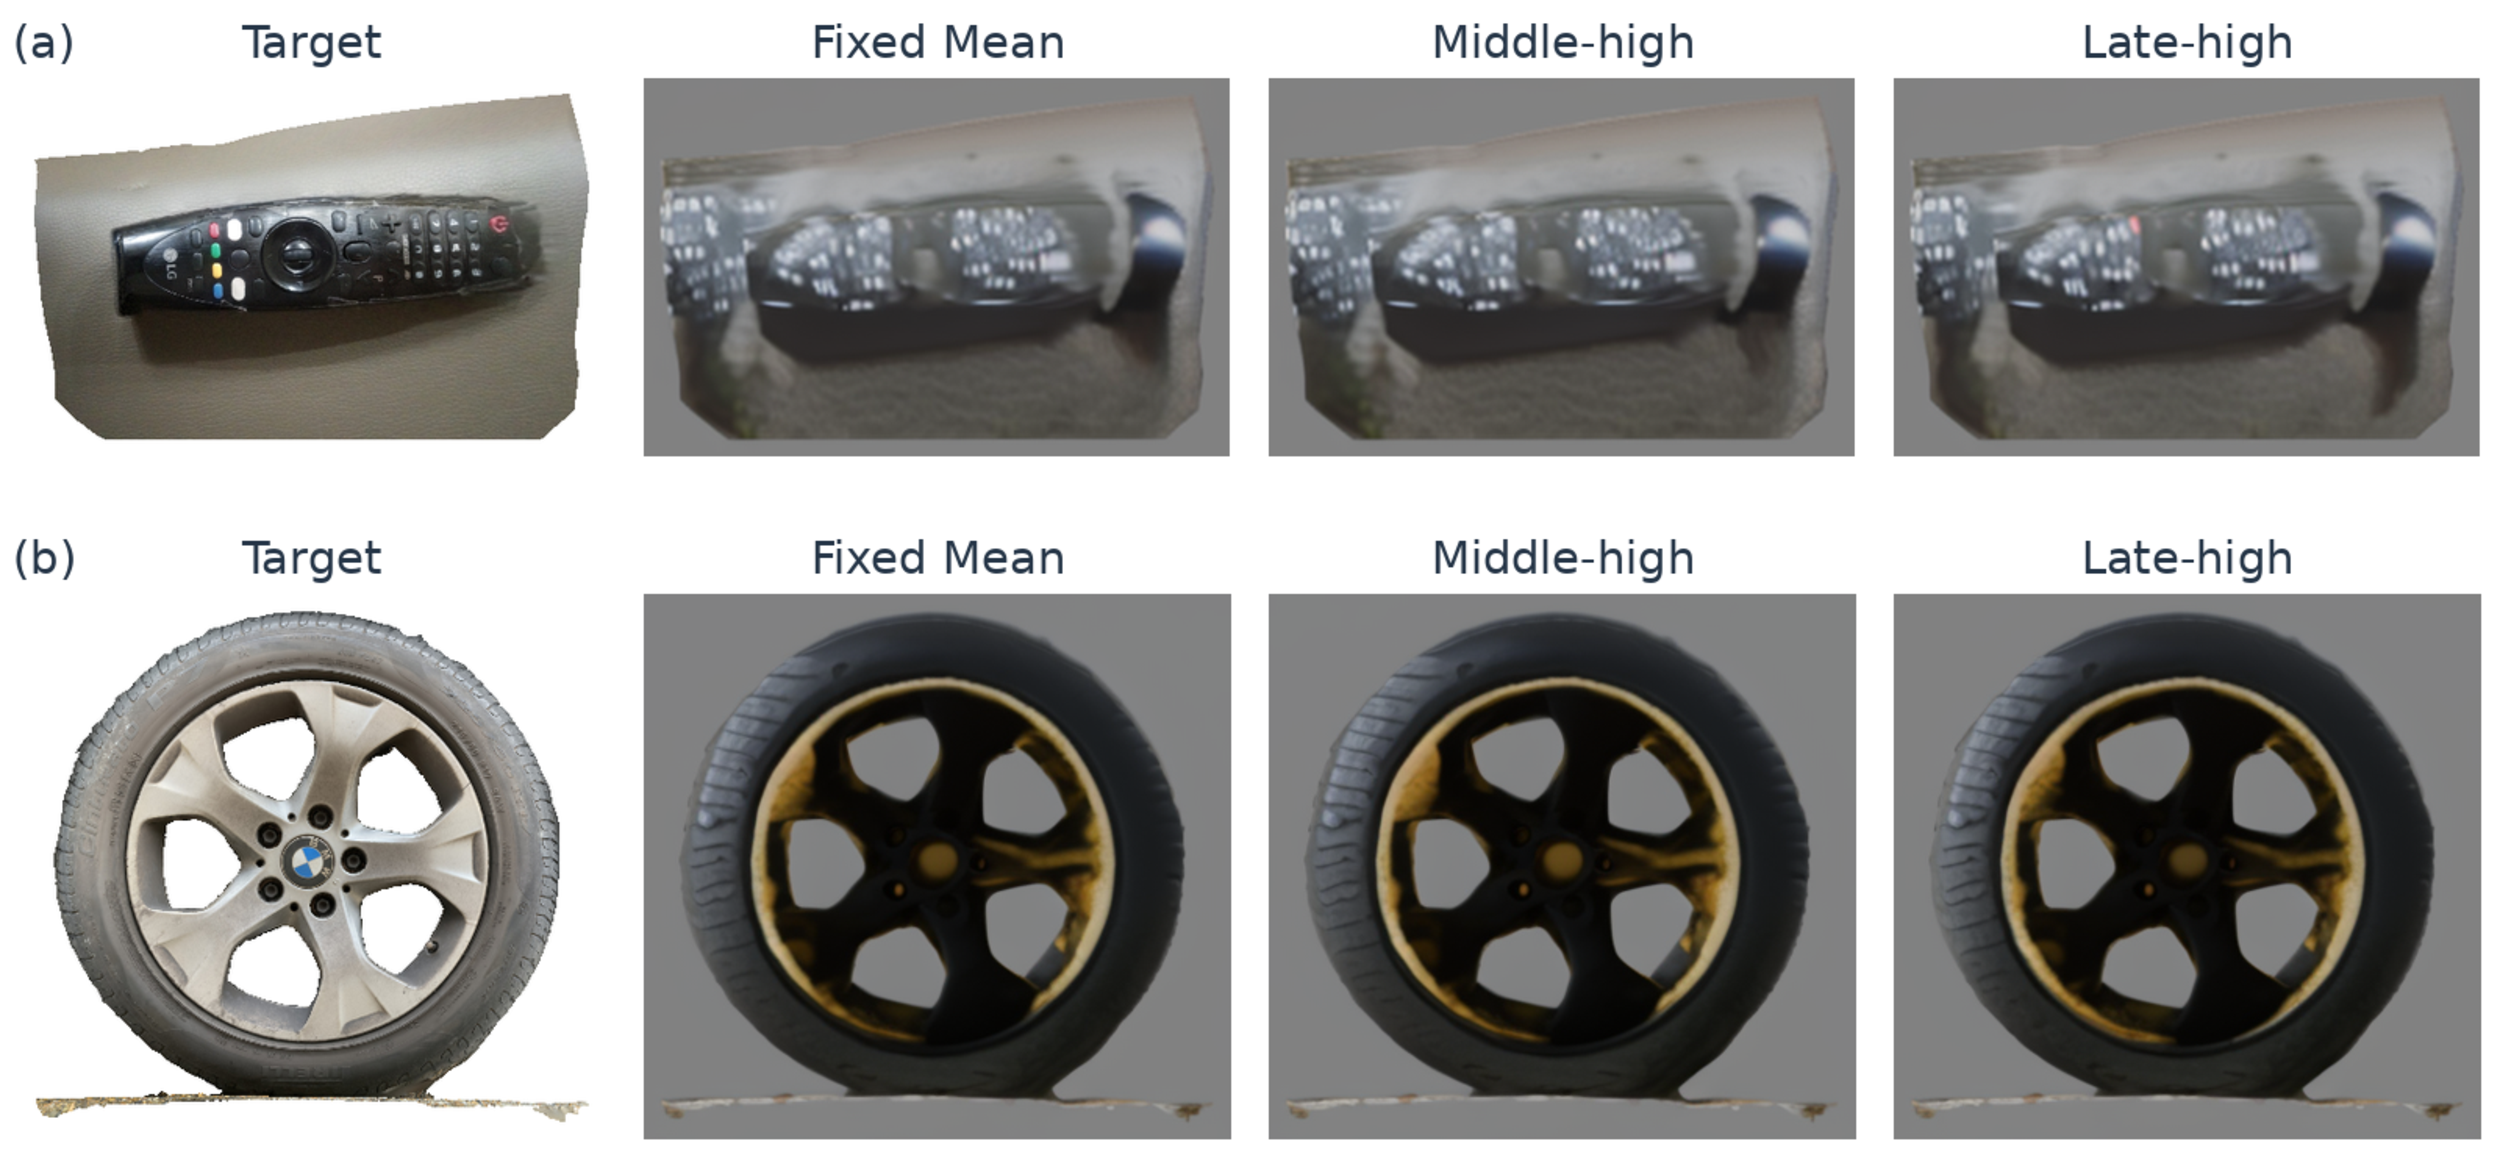
\includegraphics[width=\textwidth]{figures/fig9_mvadapter_native014.pdf}
\caption{\DIFaddFL{Native MV-Adapter view 0 for the same first two input-order rights-cleared objects: (a) LG Remote, (b) Tire. Target, Fixed Mean, Middle-high and Late-high use the native camera, object seed and a common complete-object frame. Original backgrounds and research pixels are retained. The remote preserves recognizable details while the tire retains a marked appearance mismatch; the neighboring scheduling outputs are visually similar. These illustrative cases do not establish cross-interface superiority; the fifty-object primary interval includes zero. All seven controls are displayed in Supplementary Section~S3. Credits: mohd.akmal.mahyudin and Koto3D Stephane Vogley, CC Attribution (Supplementary Sections~S5 and S9).}}
\label{fig:native50-visual}
\end{figure*}
\DIFaddend 

\DIFdelbegin \DIFdel{As shown in Table~\textit{[removed reference: }\texttt{tab:retention}\textit{]}, compared with conservative scaling $s = 1.25$, aggressive scaling $s = 2.50$ retains only 67.8\% of Laplacian variance, 64.3\% of RGB standard deviation, and 80.7\% of gradient magnitude, indicating that full high-scale scaling substantially weakens foreground color variation and high-frequency details. In contrast, C3 retains 83.5\%, 97.0\%, and 88.3\% of these metrics, respectively, and clearly outperforms $s = 2.50$ across all three texture measures. This shows that TCAS still incurs some texture reduction, but it substantially alleviates texture flattening compared with full high-scale scaling}\DIFdelend \DIFaddbegin \paragraph{External-input native schedule comparison.}
\DIFadd{The source-ordered GSO100 convenience cohort uses the same native MV-Adapter control path and three shared seeds. Native/Fixed High, Fixed Low, Fixed Mean, Early-high, Middle-high, Late-high and Generic Linear include the four inherited profiles frozen before their outputs, after earlier baseline exposure. The full dataset contains 3,600 generated cells and 21,600 view records, including three archived projection corrections and two separately frozen APG baselines \cite{sad2024apg}. The scheduling extension is external sensitivity, not pristine independent confirmation or parameter search}\DIFaddend .

\DIFdelbegin \DIFdel{Object-level statistics further show that C3 outperforms $s = 2.50$ on 87.7\%, 95.0\%, and 83.0\% of objects in Laplacian variance, RGB standard deviation, and gradient magnitude, respectively. The corresponding bootstrap 95\% confidence intervals do not cross zero, indicating statistically stable texture-preservation advantages. C3 also outperforms $s = 2.50$ on 74.3\% of objects in PSNR. By contrast, the confidence interval for the FG-SSIM difference includes zero, so these data do not establish a significant difference in foreground structural similarity between C3 and $s = 2.50$. Therefore, TCAS does not noticeably sacrifice structural alignment, while significantly reducing the texture degradation caused by full high-scale scaling}\DIFdelend \DIFaddbegin \DIFadd{The specified all-six-view Middle-high minus Fixed Mean primary is $-0.014$ dB (interval $[-0.031,+0.004]$; paired $p=0.122$)}\DIFaddend . \DIFaddbegin \DIFadd{A secondary Late-high--Fixed Mean contrast is $+0.045$ dB ($[+0.024,+0.065]$; Holm83 $p=0.00335$), with SSIM $+0.00134$ (adjusted $p=0.000415$). Its five-nonreference-view LPIPS difference is $-0.000086$ ($[-0.000551,+0.000413]$; separate Holm21 $p=1$). Thus a small detected image effect does not establish a perceptual or baked-appearance benefit. Table~\ref{tab:interface-effects} and Figure~\ref{fig:allocation-effects} put these named comparisons in context.
}\DIFaddend 

\DIFdelbegin \DIFdel{In summary, the 300-object experiments demonstrate that adapter scaling affects both structural alignment and texture detail preservation. Full high-scale scaling strengthens edge constraints but is more likely to cause texture flattening. TCAS strengthens geometric correction in the middle stage and reduces adapter intervention in the late stage, thereby maintaining structural alignment while substantially reducing texture loss. It should be noted that C3 still has some texture decrease relative to $s = 1.25$; therefore, we do not claim that TCAS completely eliminates texture loss, but rather that it significantly reduces texture degradation compared with full high-scale scaling. }%DIFDELCMD < 

%DIFDELCMD < \paragraph{Perceptual evaluation with CLIP-IQA}
%DIFDELCMD < %%%
\DIFdel{To address the concern that proxy texture statistics do not directly measure perceptual quality, we additionally evaluate CLIP-IQA \textit{[removed citation: }\texttt{wang2023clipiqa}\textit{]}, which builds on CLIP image--text representations \textit{[removed citation: }\texttt{radford2021clip}\textit{]}, on a 50-object subset of the evaluation pool as a complementary no-reference perceptual signal. CLIP-IQA is used as complementary perceptual evidence rather than a complete replacement for human preference evaluation.
}\DIFdelend \DIFaddbegin \begin{table*}[t]\centering\scriptsize\setlength{\tabcolsep}{3pt}
\caption{Selected within-study paired effects. P: the specified primary, unadjusted within its study; S: secondary with its original family adjustment (GSO all-six Holm83, nonreference LPIPS Holm21, reference-protocol secondary Holm18). Intervals are pointwise. Native50 and GSO100 use different inputs/seed policies; the reference-protocol study also changes weights and sampling and is not a separate backbone.}
\label{tab:interface-effects}
\begin{tabular}{lllrrcr}
\toprule Study & Contrast & Endpoint & Mean & 95\% CI & Class & $p$ \\
\midrule
Native MV-Adapter50 & Middle--Mean & FG-PSNR & +0.029 & [-0.019,+0.081] & P & 0.281 \\
GSO100 & Middle--Mean & FG-PSNR & -0.014 & [-0.031,+0.004] & P & 0.122 \\
GSO100 & Late--Mean & FG-PSNR & +0.045 & [+0.024,+0.065] & S & 0.003 \\
GSO100 & Late--Mean & Nonref LPIPS & -0.000086 & [-0.000551,+0.000413] & S & 1.000 \\
Reference-protocol50 & Late--Mean & Nonref PSNR & -1.184 & [-1.587,-0.849] & S & $<0.0001$ \\

\bottomrule\end{tabular}\end{table*}
\DIFaddend 

\DIFdelbegin %DIFDELCMD < \begin{table}[t]
%DIFDELCMD < \centering
%DIFDELCMD < \caption{CLIP-IQA perceptual evaluation on 50 objects from the evaluation pool. Scores are reported for foreground regions and full rendered views; $\pm$ denotes the standard deviation across the 50 objects. Higher is better.}
%DIFDELCMD < \label{tab:clipiqa}
%DIFDELCMD < \footnotesize\setlength{\tabcolsep}{4pt}
%DIFDELCMD < \begin{tabular}{lccc}
%DIFDELCMD < \toprule
%DIFDELCMD < Method & CLIP-IQA (FG)$\uparrow$ & CLIP-IQA (Full)$\uparrow$ & Win vs. $s=2.50$ \\
%DIFDELCMD < \midrule
%DIFDELCMD < $s = 1.25$ & $\mathbf{0.4920 \pm 0.0032}$ & $\mathbf{0.4918 \pm 0.0030}$ & $\mathbf{98.0\%}$ \\
%DIFDELCMD < $s = 2.50$ & $0.4860 \pm 0.0018$ & $0.4857 \pm 0.0017$ & -- \\
%DIFDELCMD < C3 (TCAS) & $0.4906 \pm 0.0028$ & $0.4903 \pm 0.0025$ & 94.0\% \\
%DIFDELCMD < \bottomrule
%DIFDELCMD < \end{tabular}
%DIFDELCMD < \end{table}
%DIFDELCMD < %%%
\DIFdelend \DIFaddbegin \begin{figure*}[t]\centering
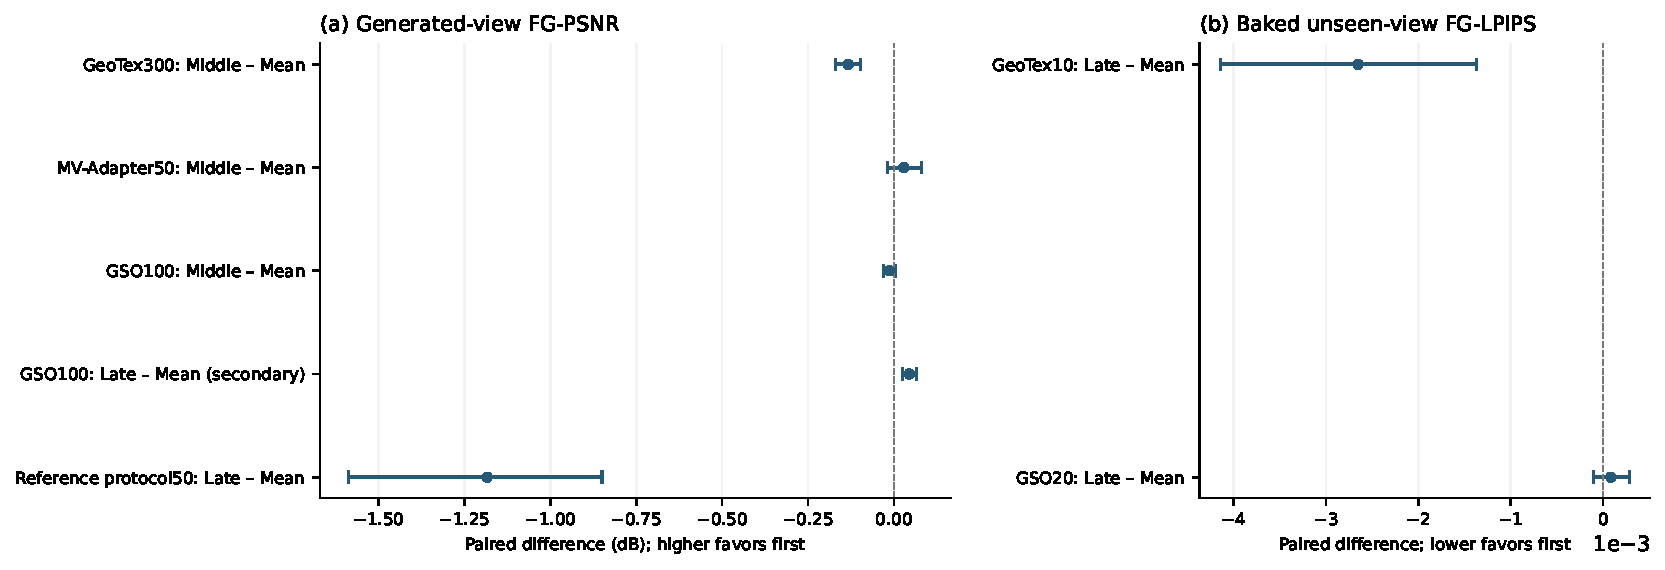
\includegraphics[width=\textwidth]{figures/fig_allocation_effects014.pdf}
\caption{\DIFaddFL{Paired allocation effects from completed object-level records. Error bars are pointwise 95\% object intervals. Panel (a) uses Fresh C composite PSNR and native-interface mean-view PSNR; the reference-protocol row excludes its reference view; panel (b) uses eleven unseen baked views. The GSO Late--Mean PSNR row is secondary and is explicitly distinguished from the specified middle-window questions. Different studies are shown separately, without pooling or cross-pipeline absolute-score ranking. The small GeoTex bake gain and GSO non-detection both remain visible.}}
\label{fig:allocation-effects}
\end{figure*}
\DIFaddend 

\DIFdelbegin \DIFdel{Table~\textit{[removed reference: }\texttt{tab:clipiqa}\textit{]} shows that C3 achieves a foreground CLIP-IQA score of 0.4906 versus 0.4860 for $s = 2.50$, scoring higher on 47 of the 50 objects (94.0\%).
The paired comparison uses a two-sided paired $t$-test over objects ($t(49)=10.52$, $p\approx3.6\times10^{-14}$), }\DIFdelend \DIFaddbegin \paragraph{Fixed-seed sensitivity.}
\DIFadd{A post-inspection analysis retains all three recorded sampling seeds. GSO100 Late--Mean PSNR averages are positive at each seed ($+0.057,+0.038,+0.039$ dB), but only 27/100 objects improve at all three }\DIFaddend and \DIFdelbegin \DIFdel{the 95\% confidence interval of the paired mean difference is constructed by }\DIFdelend \DIFaddbegin \DIFadd{68/100 have mixed or tied directions. Its nonreference LPIPS averages change direction ($-0.000389,-0.000269,+0.000398$). For the GSO20 bake, only 1/20 objects has lower Late--Mean LPIPS at all three seeds; 14/20 have mixed or tied directions. Sign agreement has no practical-effect threshold. These conditional, }\DIFaddend object-level \DIFdelbegin \DIFdel{percentile bootstrap with 10}%DIFDELCMD < {%%%
\DIFdel{, }%DIFDELCMD < }%%%
\DIFdel{000 resamples,giving $[0.0037,\,0.0054]$,which excludes zero. The ordering $s = 1.25$ $>$ C3 $>$ $s = 2.50$ supports the diagnosis that aggressive scaling reduces perceptual quality, while TCAS recovers most of this loss with stronger geometry than conservative scaling.
}%DIFDELCMD < 

%DIFDELCMD < \paragraph{Blinded preference study}
%DIFDELCMD < %%%
\DIFdel{To further examine whether the diagnostic texture differences are perceptually meaningful, we conducted a blinded three-alternative forced-choice (3AFC)preference study on 30 objects drawn from the evaluation pool. Twenty-four participants viewed, for each object and each of the three criteria (texture naturalness, shape consistency, overall quality), the anonymized outputs of conservative uniform scaling, aggressive uniform scaling, and C3 side by side; the left-to-right order of the three conditions was randomized independently per trial, and participants were not informed which method produced which image or how many conditions existed. Instructions asked participants to select the best image for the stated criterion only . Each participant judged all 30 objects for all three criteria, yielding 720 valid first-choice decisions for each criterion. The study complements the proxy diagnostics by testing whether the observed texture and structure differences are reflected in human preference}\DIFdelend \DIFaddbegin \DIFadd{summaries do not estimate training randomness or revise the original primary tests; full seed intervals and deltas are in Supplementary Section~S4}\DIFaddend .

\DIFdelbegin %DIFDELCMD < \begin{table}[!htbp]
%DIFDELCMD < \centering
%DIFDELCMD < \caption{Blinded three-alternative first-choice preference study. Percentages are computed over 720 valid decisions per criterion.}
%DIFDELCMD < \label{tab:preference}
%DIFDELCMD < \footnotesize\setlength{\tabcolsep}{3.5pt}
%DIFDELCMD < \begin{tabular}{lccc}
%DIFDELCMD < \toprule
%DIFDELCMD < Method & Texture naturalness$\uparrow$ & Shape consistency$\uparrow$ & Overall quality$\uparrow$ \\
%DIFDELCMD < \midrule
%DIFDELCMD < $s = 1.25$ & $\mathbf{332/720\ (46.1\%)}$ & 96/720 (13.3\%) & 176/720 (24.4\%) \\
%DIFDELCMD < $s = 2.50$ & 104/720 (14.4\%) & $\mathbf{331/720\ (46.0\%)}$ & 126/720 (17.5\%) \\
%DIFDELCMD < C3 (TCAS) & 284/720 (39.4\%) & 293/720 (40.7\%) & $\mathbf{418/720\ (58.1\%)}$ \\
%DIFDELCMD < \bottomrule
%DIFDELCMD < \end{tabular}
%DIFDELCMD < \end{table}
%DIFDELCMD < \FloatBarrier
%DIFDELCMD < 

%DIFDELCMD < %%%
\DIFdel{The preference pattern in Table~\textit{[removed reference: }\texttt{tab:preference}\textit{]} follows the intended trade-off. Conservative scaling is most often selected for texture naturalness, while aggressive scaling is most often selected for shape consistency. C3 stays close to both single-scale baselines on their respective strengths and receives the highest overall preference, with 58.1\% of all overall-quality votes. Thus, TCAS is not claimed to maximize every individual criterion; it provides a perceptually preferred balance between geometric adherence and texture preservation}\DIFdelend \DIFaddbegin \DIFadd{All fifteen specified GSO projection-minus-baseline nonreference-LPIPS comparisons favor the scale/APG baselines after their original separate Holm9/Holm6 corrections. The three projection candidates also lose to native on baked LPIPS in the retained twenty-object family. These valid negative auxiliary results are reported completely in Supplementary Sections~S4 and S8; they are not proposed as additional methods}\DIFaddend .

\DIFdelbegin \DIFdel{Because first-choice decisions are clustered within both participants and objects , we additionally report 95\% confidence intervals obtained by a two-level cluster bootstrap (resampling participants and objects with replacement, 10}%DIFDELCMD < {%%%
\DIFdel{,}%DIFDELCMD < }%%%
\DIFdel{000 resamples). }\DIFdelend \DIFaddbegin \subsection{Historical Preference and Training Evidence}
\label{subsec:preference}
\DIFadd{The original blinded 3AFC study on thirty objects and twenty-four participants reports }\DIFaddend C3's overall-quality share \DIFdelbegin \DIFdel{is }\DIFdelend \DIFaddbegin \DIFadd{as }\DIFaddend 58.1\% (\DIFdelbegin \DIFdel{95\% CI $[50.1\%, 65.8\%]$), exceeding the conservative and aggressive baselines by $+33.6$ (CI $[19.3, 47.2]$) and $+40.6$ percentage points (CI $[29.4, 51.8]$); both differences exclude zero, so the overall-preference advantage of C3 is significant under cluster-aware inference. By contrast, the baselines' single-criterion advantages are not significant (texture naturalness: $s = 1.25$ over C3 $+6.7$ points, CI $[-7.9, 21.5]$; shape consistency: $s = 2.50$ over C3 $+5.3$ points, CI $[-6.7, 17.9]$). Overall quality is therefore the only criterion with a significant preference, supporting the interpretation of TCAS as the perceptually preferred balance rather than a per-criterion maximum.
}%DIFDELCMD < 

%DIFDELCMD < \subsection{FAC Adaptive Correction Extension: A Controlled Re-examination}
%DIFDELCMD < \label{subsec:facexp}
%DIFDELCMD < 

%DIFDELCMD < %%%
\DIFdel{TCAS uses a fixed three-stage scale, which has the advantages of requiring no training, being simple to implement, and introducing low computational overhead. However, its residual scaling is still uniform across spatial positions and frequency components, lacking fine-grained adaptivity.
To examine whether stage-wise adapter control can be extended to learned adaptive correction, we trained the FAC extension---LTAG for timestep gating, GSG for spatial gating, and FSC for frequency-selective correction on top of the TCAS temporal schedule. The base model, VAE, and GeoTex-Adapter remain frozen; only the three lightweight controllers are trainable, adding roughly $6\times10^{3}$ parameters. The controllers are trained with the same enhanced denoising objective as the base adapter---a latent noise-prediction MSE with $1.7\times$ foreground and $1.3\times$ edge spatial reweighting plus a latent-SSIM term---using AdamW (peak learning rate $10^{-4}$, 100 warm-up steps) for 2}%DIFDELCMD < {%%%
\DIFdel{,}%DIFDELCMD < }%%%
\DIFdel{000 steps on the adapter's training pool , which is strictly disjoint from all evaluation objects, and all variants are evaluated on the strong-residual, per-layer-capped adapter instance of Section~\textit{[removed reference: }\texttt{subsec:adapterdep}\textit{]} under a strictly paired protocol (identical objects,seeds, and evaluation code).
}\DIFdelend \DIFaddbegin \DIFadd{two-level participant/object-bootstrap interval $[50.1,65.8]\%$). This supports overall preference for the original stimuli, not texture fidelity, the retrained checkpoint or unseen baked appearance. Counts and endpoint-specific results are retained in Supplementary Section~S7.
}\DIFaddend 

\DIFdelbegin \DIFdel{In this controlled setting, no learned variant reached the training-free schedule. We tested seven configurations spanning the most favorable training conditions we could construct: joint training of all controllers; a two-stage scheme with the temporal gate warm-started at the exact C3 envelope and frozen while the spatial and frequency controllers train; an envelope penalty that constrains the gate to remain near C3 during joint training; a fidelity-weighted objective; and a gently scheduled variant with fourfold-reduced training. Their paired deficits relative to the TCAS baseline range from $-1.1$ to $-2.9$~dB foreground PSNR (FG-PSNR; win rates at most 16\%), increasing monotonically with the amount of controller training. A warm-start control in which the gate is left untrained at the exact C3 envelope is statistically indistinguishable from TCAS (paired }\DIFdelend \DIFaddbegin \paragraph{FAC re-examination.}
\label{subsec:facreported}
\DIFadd{Previously reported FAC configurations all reduced }\DIFaddend FG-PSNR \DIFdelbegin \DIFdel{$\Delta=-0.18$~dB on the 12-object control, 95\% CI $[-0.42,+0.05]$, crossing zero), validating the evaluation path. No configuration or hyperparameter was selected on any evaluation object; the complete dose--response study over all seven configurations is provided in the supplementary material. }%DIFDELCMD < 

%DIFDELCMD < %%%
\DIFdel{For transparency, we note that an initial evaluation of the FAC extension, conducted on the main adapter under our earlier protocolbefore the strictly paired and strictly disjoint training controls were adopted, had suggested a positive gain. That initial comparison differed in both evaluation protocol and adapter instance, and it does not meet the controls we now consider necessary for a transfer claim; under the strictly paired, strictly disjoint protocolabove, no trained configuration replicates the gain. We therefore report only the controlled re-examination and treat the initial comparison as superseded. }%DIFDELCMD < 

%DIFDELCMD < %%%
\DIFdel{The outcome delimits the scenario in which learned modulation affects the paper's conclusions. Preserving the temporal envelope is necessary but not sufficient: with the envelope preserved and the controllers untrained, the extension neither helps nor harms, while every trained configuration degraded fidelity, indicating that the remaining damage is driven by the learned-modulation training signal itself, which trades foreground fidelity for denoising-objective loss . Learning a modulation that improves upon the C3 schedule therefore requires a training signal that does not trade away foreground fidelity (e.g.
, fidelity-weighted objectives, envelope-preserving constraints, or post-hoc rather than gradient-learned gates), which we identify as future work. With the tested lightweight controllers, the fixed schedule is the stronger default , and TCAS, which is training-free and plug-and-play, remains the main and sole method of this paper. }\DIFdelend \DIFaddbegin \DIFadd{relative to TCAS in their stated controlled re-examination. The original training pool was reported as 1,706 objects, while a recovered configuration refers to 1,200; seed, checkpoint and sampled-run records are incomplete. The results and reproducible inference/statistical components are separated from this remaining training-replay gap in Supplementary Section~S7. Recovered FAC source is now supplied with standalone controller checks. An earlier entry requires an explicit flag to freeze the base adapter, whereas the later entry freezes it by construction; the executed historical source/CLI cannot be authenticated from their names. Later new geometry training does not restore historical FAC identity.
}\DIFaddend 


\FloatBarrier
\DIFaddbegin \section{Discussion and Limitations}
\label{sec:limitations}
\DIFaddend 

\DIFdelbegin %DIFDELCMD < \subsection{Adapter-Dependence of High-Scale Failure Modes}
%DIFDELCMD < \label{subsec:adapterdep}
%DIFDELCMD < 

%DIFDELCMD < %%%
\DIFdel{The preceding experiments demonstrate the texture-flattening failure mode under high adapter scaling on the studied adapter checkpoint. A natural question is whether this failure mode is universal or specific to the adapter's trained residual properties. We conduct additional analysis across adapter checkpoints with different residual magnitudes to characterize how the failure mode depends on adapter properties. }%DIFDELCMD < 

%DIFDELCMD < %%%
\DIFdel{We find that the specific failure mode of aggressive adapter scaling is not universal. Across three adapter checkpoints spanning a spectrum of trained residual magnitudes, uniform high scale ($s = 2.50$) produced: (a) texture flattening when all layers are scaled without per-layer caps; (b) high-frequency artifact amplification when per-layer caps restrict the fine-texture layer to a low scale while coarse layers are boosted; or (c) no appreciable effect when the adapter's residual magnitude is very small. A per-layer scale-cap ablation on the same checkpoint reproduced both (a) and (b), isolating the inference-time scale semantics as the determining factor for the failure \emph{direction}.
}%DIFDELCMD < 

%DIFDELCMD < %%%
\DIFdel{A residual-magnitude sweep further shows that the intervention \emph{strength} is monotonic in the trained residual magnitude: scaling the adapter's output projection from 0.1$\times$ to 3$\times$ transitions the behavior from no-effect, to artifact amplification under high scale, to over-constraint even under conservative scale}\DIFdelend \DIFaddbegin \paragraph{What the controls establish.}
\DIFadd{The Fresh C300 gain over fixed low supports the recorded intervention under its frozen protocol}\DIFaddend . \DIFaddbegin \DIFadd{It changes both budget and timing. The equal-applied-budget matrix then measures a timing-allocation total effect and changes the preferred image-space operating point. It does not identify a state-independent residual dose or an optimal middle window. Competitive fixed and linear controls are necessary before assigning practical value to a selected profile.
}\DIFaddend 

\DIFdelbegin \DIFdel{Moreover, a six-object stage ablation shows that even \emph{which denoising stage is most sensitive to high scale} is adapter-dependent: on the artifact-prone adapter, early-stage high scale reproduced nearly all of the damage (FG-SSIM $\downarrow$ from 0.266 to 0.187) while late-stage high scale was nearly harmless (}\DIFdelend \DIFaddbegin \paragraph{Application value and operating points.}
\DIFadd{In the GeoTex image protocol, Fixed High and Generic Linear have stronger endpoint means than C3; equal-budget late-high trades higher PSNR and lower LPIPS against lower }\DIFaddend FG-SSIM \DIFdelbegin \DIFdel{0.261), whereas on the paper's main adapter the late stage was the primary source of texture loss.
}\DIFdelend \DIFaddbegin \DIFadd{than fixed mean. The ten-object bake's approximately 2\% LPIPS reduction closes only 3.7\% of the gap to the matched GT reference bake, while visible appearance errors remain. The separate GSO20 study does not detect that allocation benefit. Its post hoc calibration, GT self-bake loss and incomplete coverage are disclosed; a small image effect alone does not justify replacing an existing deployment setting.
}\DIFaddend 

\DIFdelbegin \DIFdel{Despite this variability, in every regime where scaling had a non-negligible effect, the temporal low-high-low schedule C3 yielded the best shape-texture balance. This indicates that TCAS's value is structural rather than incidental: by relying on the diffusion process's stage-dependent roles (global layout $\to$ geometry refinement $\to$ texture synthesis), it mitigates the harm of high-scale intervention across the tested adapter regimes, despite their adapter-specific failure modes. The failure mode (flatten vs. \ artifact vs. \ no-op), its strength, }\DIFdelend \DIFaddbegin \DIFadd{The evidence suggests a practical evaluation sequence rather than a new selection algorithm: compare native/default }\DIFaddend and \DIFdelbegin \DIFdel{its temporal location are all adapter-dependent; what remains stable in our experiments is that the middle denoising stage was the best-performing tested window for geometric correction, although whether this holds across adapter families remains an open question for future work.
}\DIFdelend \DIFaddbegin \DIFadd{competitive fixed settings inside the same deployed protocol; use matched applied budgets to assess timing; check reference appearance and the actual unseen-view bake; and repeat the named comparison across fixed seeds before claiming repeatable objectwise improvement. The tested GeoTex image setting supports stronger fixed controls than historical C3. The native-interface and GSO bake results provide no general reason to replace a deployment's fixed setting with the middle window. These bounded conclusions do not depend on a universally winning schedule.
}\DIFaddend 

\DIFdelbegin \DIFdel{Two further robustness checks were performed on the strong-residual, per-layer-capped adapter instance described above. First, a boundary/peak sensitivity sweep (three high-scale windows $[0.25,0.75)$, $[1/3,2/3)$, $[0.4,0.6)$ $\times$ five peak scales from 2.00 to 3.00, fifteen candidates on the 24-object probe protocol) shows that the canonical middle-third window lies in the stable high-performance region: its 2.50 setting achieves 16.71~dB whole-image PSNR, the best setting in the same window (2.75) achieves 16.79~dB with worse texture diagnostics and lower FG-SSIM, and the broader and narrower windows reach at most 16.73 and 16.62~dB. C3 is therefore a robust middle-stage choice rather than a boundary-sensitive point estimate. Second, because the 24-object probe is part of the 300-object pool, transfer claims were re-verified on the disjoint 276-object holdout ($\mathrm{obj}_{0024}$--$\mathrm{obj}_{0299}$), summarized in Table~\textit{[removed reference: }\texttt{tab:holdoutsched}\textit{]}: C3 improves PSNR over the strongest non-C3 probe candidates by $+0.258$~dB (95\% CI $[0.207,0.308]$, 206/276 wins) over a trapezoid schedule and $+0.324$~dB ($[0.281,0.367]$, 232/276 wins) over a Gaussian-peak schedule, and over the reviewer-relevant generic schedules by $+0.323$~dB ($[0.263,0.386]$, 214}\DIFdelend \DIFaddbegin \DIFadd{Generated-view metrics remain informative: overall baked}\DIFaddend /\DIFdelbegin \DIFdel{276 wins, FG-SSIM statistically tied) over linear warm-up and $+0.902$~dB ($[0.824,0.981]$, 253}\DIFdelend \DIFaddbegin \DIFadd{image method rankings are positively associated. However, preferred point estimates often change, and the association is weaker when the GSO analysis is restricted to closely competing scale}\DIFaddend /\DIFdelbegin \DIFdel{276 wins, FG-SSIM $+0.046$) over the cosine bump. The holdout ordering matches the probe: warm-up approaches C3 in structure but loses in signal fidelity, and the smooth bump loses in both because its effective high-scale duration is shorter than the full middle third}\DIFdelend \DIFaddbegin \DIFadd{time settings. Winner changes do not prove significant separation between methods or a general reversal. Actual baked evaluation and full-object reference comparison remain necessary}\DIFaddend .

\DIFdelbegin %DIFDELCMD < \begin{table}[t]
%DIFDELCMD < \centering
%DIFDELCMD < \caption{Scheduling transfer on the disjoint 276-object holdout ($\mathrm{obj}_{0024}$--$\mathrm{obj}_{0299}$; strong-residual, per-layer-capped adapter instance of Section~\textit{[removed reference: }\texttt{subsec:adapterdep}\textit{]}). $\Delta$PSNR (dB) is the paired C3-minus-competitor difference (positive favors C3); 95\% CIs use object-level percentile bootstrap with 10{,}000 resamples. Absolute metrics are means over holdout objects and views.}
%DIFDELCMD < \label{tab:holdoutsched}
%DIFDELCMD < \footnotesize\setlength{\tabcolsep}{2.5pt}
%DIFDELCMD < \begin{tabular}{lcccc}
%DIFDELCMD < \toprule
%DIFDELCMD < Schedule & FG-SSIM$\uparrow$ & PSNR$\uparrow$ & $\Delta$PSNR vs.\ C3 (95\% CI) & C3 wins \\
%DIFDELCMD < \midrule
%DIFDELCMD < Trapezoid & 0.356 & 19.04 & $+0.258$ $[0.207, 0.308]$ & 206/276 \\
%DIFDELCMD < Gaussian peak & 0.358 & 18.97 & $+0.324$ $[0.281, 0.367]$ & 232/276 \\
%DIFDELCMD < Linear warm-up & 0.377 & 18.97 & $+0.323$ $[0.263, 0.386]$ & 214/276 \\
%DIFDELCMD < Cosine bump & 0.330 & 18.39 & $+0.902$ $[0.824, 0.981]$ & 253/276 \\
%DIFDELCMD < C3 (TCAS) & 0.376 & 19.29 & -- (reference) & -- \\
%DIFDELCMD < \bottomrule
%DIFDELCMD < \end{tabular}
%DIFDELCMD < \end{table}
%DIFDELCMD < 

%DIFDELCMD < \section{Limitations}
%DIFDELCMD < \label{sec:limitations}
%DIFDELCMD < 

%DIFDELCMD < %%%
\DIFdel{This paper mainly focuses on inference-time adapter scaling and does not retrain the base multi-view diffusion model or the adapter. Therefore, TCAS can alleviate texture degradation under high scales---which may manifest as flattening or artifact amplification depending on the adapter's residual properties---but it cannot fundamentally solve the limitations of the base model in invisible-region completion, complex material synthesis, and cross-view detail consistency. }%DIFDELCMD < 

%DIFDELCMD < %%%
\DIFdel{Second, Laplacian variance, RGB standard deviation, and gradient magnitude are proxy metrics for texture degradation. They are effective for detecting high-frequency loss and surface smoothing, but they cannot fully replace human perceptual evaluation. For objects with strong reflection, transparency, thin structures, or highly stylized textures, discrepancies may exist between these metrics and subjective quality.
}\DIFdelend \DIFaddbegin \paragraph{Interface and protocol boundaries.}
\DIFadd{Native MV-Adapter50 and GSO100 do not detect the primary middle-window advantage. The secondary GSO late-window PSNR change is statistically detectable but small, with no corresponding nonreference LPIPS benefit. The supporting reference-conditioned checkpoint shows a different Late--Mean direction. Historical MVDiffusion supplies a partial-operator boundary. Because weights, inputs, conditioning operators and sampling protocols differ, these studies cannot isolate one backbone or domain as the cause of the varying effects.
}\DIFaddend 

\DIFdelbegin \DIFdel{In addition, the current TCAS uses fixed stage boundaries and a fixed scale combination, C3 = (1.25, 2.50, 1.25).
This setting is simple and stable, but it should be understood as a validated inference strategy for the studied geometry-adapter pipeline rather than a universally optimal schedule. As shown in Section~\textit{[removed reference: }\texttt{subsec:adapterdep}\textit{]}, the failure mode of high-scale intervention is adapter-dependent, }\DIFdelend \DIFaddbegin \paragraph{Quality, selection and replication limits.}
\DIFadd{The bake studies favor compatible native-UV assets, and GSO uses a source-ordered convenience sample. They do not establish representative asset quality, physical albedo, PBR fidelity or a validated seam score. Views and seeds are nested within object, }\DIFaddend and \DIFdelbegin \DIFdel{even the most sensitive denoising stage differs across adapters; yet C3's middle-stage concentration was the best-performing schedule among all tested variants in every regime examined, suggesting that its temporal structure is robust even when specific failure mechanisms vary. It has not yet been adapted to object complexity, material type, input reference image quality, or different sampler families, and the schedule has not yet been validated on a different geometry-conditioned multi-view diffusion backbone. Future work could study content-adaptive stage boundaries, SNR-aware scaling, and learned scale selection strategies.
}\DIFdelend \DIFaddbegin \DIFadd{seed repetitions do not estimate training-checkpoint variation. The new seed, dominance and UV-overlap summaries were proposed after observing the original outcomes and remain descriptive; their diagnostic checks do not change that chronology. Separate test families and pointwise intervals retain their stated roles; non-detection is not equivalence.
}\DIFaddend 

\DIFdelbegin \DIFdel{Finally, our controlled re-examination of the learned FAC extension indicates that unconstrained lightweight gating can flatten the temporal envelope that makes TCAS effective; learned modulation is therefore promising only under envelope-preserving constraints, which we identify as a concrete direction for future work, while TCAS remains the main training-free method.
}\DIFdelend \DIFaddbegin \DIFadd{Fresh C uses retrained weights and a controlled sampler rather than the authenticated historical main adapter or complete default pipeline. The old $+0.96$ dB contrast is not reproduced, and historical FAC training records remain incomplete. The original preference study concerns its own stimuli. These limitations constrain deployment and replication claims, while the matched within-protocol comparisons remain valid.
}\DIFaddend 

\section{Conclusion}
\label{sec:conclusion}

\DIFdelbegin \DIFdel{This paper presents a systematic experimental analysis of adapter scaling in multi-view diffusion texture generation. The experiments show that higher adapter scales continuously improve structural metrics such as FG-SSIM, but such improvement can mask texture quality degradation. In the 26-object texture audit, 92\% of objects show texture flattening and high-frequency detail loss under $s = 2.50$. This reveals an adapter-specific temporal conflict that is not captured by simply treating the scale as a generic guidance strength.
}%DIFDELCMD < 

%DIFDELCMD < %%%
\DIFdel{To address this shape-texture trade-off, we propose Timestep-Conditioned Adapter Scaling (TCAS). The selected configuration , C3, applies strong adapter correction in the middle denoising stage and uses conservative scales in the early and late stages. The 24-object probe set is used only to select C3 from 17 scaling variants that include uniform, layer-wise, and temporal alternatives. With this schedule fixed, the }\DIFdelend \DIFaddbegin \DIFadd{Geometry-control allocation changes generated-view agreement, but its effects depend on the tested interface, protocol and endpoint. The matched }\DIFaddend 300-object \DIFdelbegin \DIFdel{evaluation pool further shows that }\DIFdelend \DIFaddbegin \DIFadd{study shows that }\DIFaddend C3\DIFdelbegin \DIFdel{achieves FG-SSIM comparable to aggressive uniform scaling $s = 2.50$ while improving PSNR by 0.96~dB.
}%DIFDELCMD < 

%DIFDELCMD < %%%
\DIFdel{Therefore, the core contribution of this paper is not to claim that the generated results are visually close to the ground truth in all cases, nor to present TCAS as a universal replacement for all guidance schedules. Instead, the contribution is to reveal and validate a hidden shape-texture trade-off caused by geometry-adapter residual injection, and to show that a simple non-monotonic inference schedule can mitigate this trade-off better than fixed high-scale control and other tested scheduling variants. This conclusion suggests that, in the geometry-controlled multi-view pipeline studied here---and plausibly in similar geometry-conditioned texture pipelines---adapter strength is better treated as a stage-dependent inference control variable than as a single fixed hyperparameter. }%DIFDELCMD < 

%DIFDELCMD < %%%
\DIFdel{As an additional check, a controlled re-examination of the learned-correction extension (FAC) under a strictly paired protocol showed that unconstrained lightweight gating does not preserve the schedule's shape; the analysis delimits the scenario in which learned modulation helps---only under envelope-preserving constraints---and the training-free TCAS remains the main and sole method. }\DIFdelend \DIFaddbegin \DIFadd{'s gain over fixed low combines increased strength with timing; equal-budget fixed mean and late-high outperform the historical middle window. Native MV-Adapter studies do not detect the primary middle-window advantage, while some secondary image effects are small but measurable. Actual baking yields a limited late-high benefit on ten compatible GeoTex objects and no detected LPIPS benefit on a separate twenty-object GSO cohort. Method rankings are broadly associated across image and baked evaluation, yet their preferred operating points often differ. Competitive controls and application-level evaluation are therefore necessary when choosing a setting within a deployed pipeline. The results do not identify a universally preferred schedule or establish faithful material reproduction.
}\DIFaddend 

\section*{Data availability}

\DIFdelbegin \DIFdel{All data included in this study are available upon request by contact with the corresponding author}\DIFdelend \DIFaddbegin \DIFadd{Object-level revision metrics, frozen protocols/configuration records, verified inference and analysis scripts, and the LaTeX source required to rebuild the manuscript and Supplement are included in the author-review package. Recovered FAC source and its source/entry audit are supplied separately; standalone controller tests do not constitute historical full-model replay. The standalone reproduction archive supports statistic recomputation without model weights; fresh inference additionally requires the recorded weights, runtime and licensed source assets. The complete raw generated-image archives, trained checkpoints, and participant-level responses are not included. Source assets must be acquired under their recorded licenses; the review evidence includes attributed displays and a small licensed GSO example export. Additional analysis records may be requested from the corresponding author, subject to licensing, privacy, and archive constraints.
}

\section*{\DIFadd{Declaration of generative AI and AI-assisted technologies in manuscript preparation}}
\DIFadd{OpenAI Codex assisted with revision drafting, implementation and reproducible statistical and figure code. The final interface diagram uses reproducible vector elements; research displays come from the recorded runs without image-generation retouching. A vision-capable AI assistant inspected final figures and rendered pages for legibility and consistency with the named comparisons; this check does not certify scientific validity or replace author review. Numerical tables are computed from delivered object-level records. Final scientific review, accuracy and responsibility remain with the authors}\DIFaddend .

\section*{Declaration of competing interests}

The authors declare that they have no known competing financial interests or personal relationships that could have appeared to influence the work reported in this paper.


\DIFaddbegin \begingroup
\linespread{0.94}\selectfont
\DIFaddend \begin{thebibliography}{45}
\bibitem{liu2023zero1to3}
Liu R, Wu R, Van Hoorick B, et al. Zero-1-to-3: Zero-shot one image to 3D object. \textit{Proceedings of the IEEE/CVF International Conference on Computer Vision}, 2023.

\bibitem{shi2023zero123pp}
Shi R, Chen H, Zhang Z, et al. Zero123++: A single image to consistent multi-view diffusion base model. arXiv:2310.15110, 2023.

\bibitem{liu2023syncdreamer}
Liu Y, Lin C, Zeng Z, et al. SyncDreamer: Generating multiview-consistent images from a single-view image. \textit{International Conference on Learning Representations}, 2024.

\bibitem{long2023wonder3d}
Long X, Guo Y C, Lin C, et al. Wonder3D: Single image to 3D using cross-domain diffusion. \textit{Proceedings of the IEEE/CVF Conference on Computer Vision and Pattern Recognition}, 2024.

\bibitem{shi2024mvdream}
Shi Y, Wang P, Ye J, et al. MVDream: Multi-view diffusion for 3D generation. \textit{International Conference on Learning Representations}, 2024.

\bibitem{wang2023imagedream}
Wang P, et al. ImageDream: Image-prompt multi-view diffusion for 3D generation. arXiv:2312.02201, 2023.

\bibitem{xu2024instantmesh}
Xu J, et al. InstantMesh: Efficient 3D mesh generation from a single image with sparse-view large reconstruction models. \textit{Advances in Neural Information Processing Systems}, 2024.

\bibitem{ke2024era3d}
Li P, Liu Y, Long X, et al. Era3D: High-resolution multiview diffusion using efficient row-wise attention. \textit{Advances in Neural Information Processing Systems}, 2024.

\bibitem{chen2023text2tex}
Chen D Z, et al. Text2Tex: Text-driven texture synthesis via diffusion models. \textit{Proceedings of the IEEE/CVF International Conference on Computer Vision}, 2023.

\bibitem{richardson2023texture}
Richardson E, Metzer G, Alaluf Y, et al. TEXTure: Text-guided texturing of 3D shapes. \textit{ACM SIGGRAPH 2023 Conference Proceedings}, 2023.

\bibitem{poole2023dreamfusion}
Poole B, Jain A, Barron J T, Mildenhall B. DreamFusion: Text-to-3D using 2D diffusion. \textit{International Conference on Learning Representations}, 2023.

\bibitem{chen2023fantasia3d}
Chen R, Chen Y, Jiao N, Jia K. Fantasia3D: Disentangling geometry and appearance for high-quality text-to-3D content creation. \textit{Proceedings of the IEEE/CVF International Conference on Computer Vision}, 2023.

\bibitem{shao2025mvpainter}
Shao M, Xiong F, Sun Z, Xu M. MVPainter: Accurate and detailed 3D texture generation via multi-view diffusion with geometric control. arXiv:2505.12635, 2025.

\bibitem{kynkanniemi2024limited}
Kynk\"a\"anniemi T, Aittala M, Karras T, et al. Applying guidance in a limited interval improves sample and distribution quality in diffusion models. \textit{Advances in Neural Information Processing Systems}, 2024.

\bibitem{perla2026survey}
Perla S R K, Zhang H, Mahdavi-Amiri A. Advances in neural 3D mesh texturing: A survey. \textit{Computer Graphics Forum}, 2026, e70392.

\bibitem{guzman2026adaptive}
Guzm\'an J E, Mould D, Paquette E. Adaptive multiresolution exemplar-based texture synthesis on animated fluids. \textit{Computers \& Graphics}, 2026, 134: 104490.

\bibitem{lv2025interpretable}
Lv X, Wu Z, Xu J, et al. Interpretable procedural material graph generation via diffusion models from reference images. \textit{The Visual Computer}, 2025, 41(13): 11195--11205.

\bibitem{zeng2024paint3d}
Zeng X, Chen X, Qi Z, et al. Paint3D: Paint anything 3D with lighting-immersive texture generation. \textit{Proceedings of the IEEE/CVF Conference on Computer Vision and Pattern Recognition}, 2024.

\bibitem{cheng2024mvpaint}
Cheng W, Mu J, Zeng X, et al. MVPaint: Synchronized multi-view diffusion for painting anything 3D. \textit{Proceedings of the IEEE/CVF Conference on Computer Vision and Pattern Recognition}, 2025.

\bibitem{lai2025hunyuan3d}
Zhao Z, Lai Z, Lin Q, et al. Hunyuan3D 2.0: Scaling diffusion models for high resolution textured 3D assets generation. arXiv:2501.12202, 2025.

\bibitem{huang2024mvadapter}
Huang Z, et al. MV-Adapter: Multi-view consistent image generation made easy. \textit{Proceedings of the IEEE/CVF International Conference on Computer Vision}, 2025.

\DIFaddbegin \bibitem{tang2023mvdiffusion}
\DIFadd{Tang S, Zhang F, Chen J, Wang P, Furukawa Y. MVDiffusion: Enabling holistic multi-view image generation with correspondence-aware diffusion. \textit{Advances in Neural Information Processing Systems}, 2023.
}

\DIFaddend \bibitem{liu2024synchronized}
Liu Y X, Xie M S, Liu H Y, Wong T T. Text-guided texturing by synchronized multi-view diffusion. \textit{SIGGRAPH Asia 2024 Conference Papers}, 2024.

\bibitem{xu2026wondertex}
Xu Q, Han X G, Zhang L. WonderTex: Consistent-and-seamless texture generation with text-guided multi-view image diffusion models. \textit{IEEE Transactions on Visualization and Computer Graphics}, 2026, 32(7): 5815--5825.

\bibitem{mou2023t2iadapter}
Mou C, Wang X, Xie L, et al. T2I-Adapter: Learning adapters to dig out more controllable ability for text-to-image diffusion models. \textit{Proceedings of the AAAI Conference on Artificial Intelligence}, 2024.

\bibitem{zhang2023controlnet}
Zhang L, Rao A, Agrawala M. Adding conditional control to text-to-image diffusion models. \textit{Proceedings of the IEEE/CVF International Conference on Computer Vision}, 2023.

\bibitem{ye2023ipadapter}
Ye H, Zhang J, Liu S, Han X, Yang W. IP-Adapter: Text compatible image prompt adapter for text-to-image diffusion models. arXiv:2308.06721, 2023.

\bibitem{hu2022lora}
Hu E J, Shen Y, Wallis P, et al. LoRA: Low-rank adaptation of large language models. \textit{International Conference on Learning Representations}, 2022.

\bibitem{liu2024dora}
Liu S Y, Wang C Y, Yin H, et al. DoRA: Weight-decomposed low-rank adaptation. \textit{International Conference on Machine Learning}, 2024.

\bibitem{zhang2023adalora}
Zhang Q, Zuo S, Liang C, et al. AdaLoRA: Adaptive budget allocation for parameter-efficient fine-tuning. \textit{International Conference on Learning Representations}, 2023.

\DIFaddbegin \bibitem{kulkarni2026ssi}
\DIFadd{Kulkarni A S. Scheduled Style Injection: Expanding the Style-Content Pareto Frontier in Training-Free Diffusion-Based Style Transfer. \textit{Proceedings of the IEEE/CVF Conference on Computer Vision and Pattern Recognition Workshops (CVPRW), NTIRE Workshop}, 2026.
}

\DIFaddend \bibitem{ho2020ddpm}
Ho J, Jain A, Abbeel P. Denoising diffusion probabilistic models. \textit{Advances in Neural Information Processing Systems}, 2020.

\bibitem{song2021ddim}
Song J, Meng C, Ermon S. Denoising diffusion implicit models. \textit{International Conference on Learning Representations}, 2021.

\bibitem{ho2022cfg}
Ho J, Salimans T. Classifier-free diffusion guidance. \textit{NeurIPS Workshop on Deep Generative Models and Downstream Applications}, 2021. arXiv:2207.12598.

\bibitem{castillo2023adaptive}
Castillo A, Kohler J, P\'erez J C, et al. Adaptive guidance: Training-free acceleration of conditional diffusion models. \textit{Proceedings of the AAAI Conference on Artificial Intelligence}, 2025.

\DIFdelbegin %DIFDELCMD < \bibitem{rombach2022ldm}
%DIFDELCMD < %%%
\DIFdel{Rombach R, Blattmann A, Lorenz D, Esser P, Ommer B. High-resolution image synthesis with latent diffusion models. \textit{Proceedings of the IEEE/CVF Conference on Computer Vision and Pattern Recognition}, 2022.
}%DIFDELCMD < 

%DIFDELCMD < \bibitem{esser2024scaling}
%DIFDELCMD < %%%
\DIFdel{Esser P, Kulal S, Blattmann A, et al. Scaling rectified flow transformers for high-resolution image synthesis. \textit{International Conference on Machine Learning}, 2024.
}%DIFDELCMD < 

%DIFDELCMD < \bibitem{blackforestlabs2024flux}
%DIFDELCMD < %%%
\DIFdel{Black Forest Labs. FLUX: Flow matching for image generation. https://github.com/black-forest-labs/flux, 2024.
}%DIFDELCMD < 

%DIFDELCMD < \bibitem{loshchilov2019decoupled}
%DIFDELCMD < %%%
\DIFdel{Loshchilov I, Hutter F. Decoupled weight decay regularization. \textit{International Conference on Learning Representations}, 2019.
}%DIFDELCMD < 

%DIFDELCMD < \bibitem{cherti2023reproducible}
%DIFDELCMD < %%%
\DIFdel{Cherti M, Beaumont R, Wightman R, et al. Reproducible scaling laws for contrastive language-image learning. \textit{Proceedings of the IEEE/CVF Conference on Computer Vision and Pattern Recognition}, 2023.
}%DIFDELCMD < 

%DIFDELCMD < \bibitem{nichol2022glide}
%DIFDELCMD < %%%
\DIFdel{Nichol A, Dhariwal P, Ramesh A, et al. GLIDE: Towards photorealistic image generation and editing with text-guided diffusion models. \textit{International Conference on Machine Learning}, 2022.
}%DIFDELCMD < 

%DIFDELCMD < \bibitem{saharia2022photorealistic}
%DIFDELCMD < %%%
\DIFdel{Saharia C, Chan W, Saxena S, et al. Photorealistic text-to-image diffusion models with deep language understanding. \textit{Advances in Neural Information Processing Systems}, 2022.
}%DIFDELCMD < 

%DIFDELCMD < \bibitem{peebles2023scalable}
%DIFDELCMD < %%%
\DIFdel{Peebles W, Xie S. Scalable diffusion models with transformers. \textit{Proceedings of the IEEE/CVF International Conference on Computer Vision}, 2023.
}%DIFDELCMD < 

%DIFDELCMD < %%%
\DIFdelend \bibitem{wang2004ssim}
Wang Z, Bovik A C, Sheikh H R, Simoncelli E P. Image quality assessment: From error visibility to structural similarity. \textit{IEEE Transactions on Image Processing}, 2004, 13(4): 600--612.

\bibitem{zhang2018lpips}
Zhang R, Isola P, Efros A A, \DIFdelbegin \DIFdel{Shechtman E, Wang O}\DIFdelend \DIFaddbegin \DIFadd{et al}\DIFaddend . The unreasonable effectiveness of deep features as a perceptual metric. \textit{\DIFdelbegin \DIFdel{Proceedings of the IEEE/CVF Conference on Computer Vision and Pattern Recognition}\DIFdelend \DIFaddbegin \DIFadd{CVPR}\DIFaddend }, 2018.

\DIFdelbegin %DIFDELCMD < \bibitem{wang2023clipiqa}
%DIFDELCMD < %%%
\DIFdel{Wang J, Chan K C K, Loy C C. Exploring CLIP for assessing the look and feel of images. \textit{Proceedings of the AAAI Conference on Artificial Intelligence}, 2023.
}%DIFDELCMD < 

%DIFDELCMD < \bibitem{radford2021clip}
%DIFDELCMD < %%%
\DIFdel{Radford A, Kim J W, Hallacy C, et al. Learning transferable visual modelsfrom natural language supervision. }\DIFdelend \DIFaddbegin \bibitem{sad2024apg}
\DIFadd{Sadat S, Hilliges O, Weber R M. Eliminating oversaturation and artifacts of high guidance scales in diffusion models. }\DIFaddend \textit{International Conference on \DIFdelbegin \DIFdel{Machine }\DIFdelend Learning \DIFaddbegin \DIFadd{Representations}\DIFaddend }, \DIFdelbegin \DIFdel{2021.
}\DIFdelend \DIFaddbegin \DIFadd{2025.
}\DIFaddend 

\end{thebibliography}
\DIFaddbegin \endgroup
 \DIFaddend\end{document}
